\documentclass[12pt]{report}
\usepackage{amsmath}
\usepackage{amssymb}
\usepackage{amsfonts}
\usepackage{mathtools}
\usepackage{enumitem}
\usepackage{makecell}

\usepackage{setspace}
\usepackage[utf8]{inputenc}
\usepackage[titletoc]{appendix}
\usepackage{graphicx}
\usepackage{listings}
\graphicspath{ {Images/} {images/} }
\setlength{\parindent}{0pt}
\setlength{\parskip}{1em}
\usepackage{float}
\usepackage{multirow}
\usepackage{booktabs}
\usepackage{algorithm}
\usepackage{algpseudocode}
\usepackage{colortbl}%
  \newcommand{\myrowcolour}{\rowcolor[gray]{0.925}}
\usepackage{booktabs}
\usepackage{cite}
% hyperlinks
\usepackage{hyperref} 
\hypersetup{ colorlinks, citecolor=red, filecolor=black, linkcolor=black, urlcolor=blue } 

% blank page
\usepackage{afterpage}
\newcommand\blankpage{%
    \null
    \thispagestyle{empty}%
    \addtocounter{page}{-1}%
    \newpage}

\usepackage{pgf}
\usepackage{pgfpages}

% Border
% \pgfpagesdeclarelayout{boxed}
% {
%   \edef\pgfpageoptionborder{0pt}
% }
% {
%   \pgfpagesphysicalpageoptions
%   {%
%     logical pages=1,%
%   }
%   \pgfpageslogicalpageoptions{1}
%   {
%     border code=\pgfsetlinewidth{0.5pt}\pgfstroke,%
%     border shrink=\pgfpageoptionborder,%
%     resized width=.95\pgfphysicalwidth,%
%     resized height=.95\pgfphysicalheight,%
%     center=\pgfpoint{.5\pgfphysicalwidth}{.5\pgfphysicalheight}%
%   }%
% }
% \pgfpagesuselayout{boxed}

% page layout including header and footer
\usepackage{xcolor}
% \usepackage[a4paper,top=2cm, bottom=2cm, left=3cm, right=3cm]{geometry}
\usepackage[a4paper, left=1.25in, right=1in, top=1in, bottom=1in]{geometry}
\definecolor{myred}{HTML}{581000}
% Visible placeholder for facts only the authors can supply (ethics approval, URLs, GPU-hours).
% Every \authortodo must be resolved before submission: grep -rn authortodo Chapters main.tex
\newcommand{\authortodo}[1]{\textcolor{red}{\textbf{[AUTHORS TO FILL: #1]}}}
\usepackage{fancyhdr}
\usepackage{longtable}










% \usepackage{newtxtext,newtxmath} 
% setting the font size of chapter, title and subtitle
\usepackage[normalem]{ulem} % normalem: keep \emph as italic (not underlined)
\usepackage{lmodern}
\usepackage{sectsty}
\chapterfont{\fontsize{22pt}{22pt}\selectfont\bfseries}
\sectionfont{\fontsize{16pt}{16pt}\selectfont\bfseries}
\subsectionfont{\fontsize{14pt}{14pt}\selectfont\bfseries}

\makeatletter
\renewcommand\@seccntformat[1]{\csname the#1\endcsname\enspace} % was \quad
\makeatother

% Reduce the large blank space the report class leaves above chapter titles
% (default is 50pt of \vspace* before the chapter number).
\makeatletter
\renewcommand{\@makechapterhead}[1]{%
  \vspace*{12\p@}%
  {\parindent\z@ \raggedright \normalfont
    \ifnum \c@secnumdepth >\m@ne
        \fontsize{22pt}{26pt}\selectfont\bfseries \@chapapp\space \thechapter
        \par\nobreak \vskip 8\p@
    \fi
    \interlinepenalty\@M
    \fontsize{22pt}{26pt}\selectfont\bfseries #1\par\nobreak \vskip 26\p@}}
\renewcommand{\@makeschapterhead}[1]{%
  \vspace*{12\p@}%
  {\parindent\z@ \raggedright \normalfont
    \interlinepenalty\@M
    \fontsize{22pt}{26pt}\selectfont\bfseries #1\par\nobreak \vskip 26\p@}}
\makeatother

% %Adding footer
% % --- Fancy footer: wrapped chapter title (left) + centered page number ---
% \usepackage{fancyhdr}
% \pagestyle{fancy}
% \fancyhf{} % clear

% % --- Keep only CHAPTER info in the marks ---
% \renewcommand{\chaptermark}[1]{\markboth{#1}{}} % leftmark = chapter title
% \renewcommand{\sectionmark}[1]{}                % sections do NOT change marks
% \renewcommand{\subsectionmark}[1]{}             % (optional) subsections too

% % --- Footer: number left, page center, CHAPTER TITLE right (wrapped) ---
% \fancyfoot[L]{\textbf{Chapter \thechapter}}
% \fancyfoot[C]{\thepage}
% \fancyfoot[R]{\parbox[t]{0.45\textwidth}{\raggedleft\nouppercase{\leftmark}}}

% \renewcommand{\headrulewidth}{0pt}
% \renewcommand{\footrulewidth}{0.4pt}
% \setlength{\footskip}{28pt}

% Apply same to chapter-opening pages
% \fancypagestyle{plain}{
%   \fancyhf{}
%   \fancyfoot[L]{\textbf{Chapter \thechapter}}
%   \fancyfoot[C]{\thepage}
%   \fancyfoot[R]{\parbox[t]{0.45\textwidth}{\raggedleft\nouppercase{\leftmark}}}
%   \renewcommand{\headrulewidth}{0pt}
%   \renewcommand{\footrulewidth}{0.4pt}
% }











\usepackage{caption}
\usepackage{subcaption}
\setcounter{page}{1}
\setcounter{chapter}{0}




% table format
\usepackage{array}
\newcolumntype{Y}{>{\centering\arraybackslash}m{4.4cm}}
\newcolumntype{X}{>{\centering\arraybackslash}m{7cm}}
\newcolumntype{P}{>{\centering\arraybackslash}m{2.5cm}}
\newcolumntype{L}{>{\raggedright\arraybackslash}m{8cm}}
\newcolumntype{M}{>{\raggedright\arraybackslash}m{3.7cm}}
\newcolumntype{Z}{>{\justify}m{15cm}}

% references
%\usepackage{biblatex}
%\addbibresource{chapters/references.bib}
\renewcommand\bibname{References}

% \title{
% {End to End Bangladeshi License Plate Detection \& Recognition}}
% \author{Rashik Rahman,17201012\\Mehedi UL Hasnain,17201041\\
% Rafat Meraz,17201076\\}
% \date{2021}

% \usepackage{nomencl}    % removed: no \nomenclature entries and never \printnomenclature'd; avoids an extra makeindex pass (faster Overleaf compile)
% \makenomenclature

\begin{document}

% page no. roman
\renewcommand{\thepage}{\roman{page}}
\newcommand{\etal}{\textit{et al. }}



\begin{titlepage}
    \begin{center}
        
        % This template is created and modified by Rashik Rahman(17201012@uap-bd.edu). Feel free to contact me if you have any quarries or problems regarding this template. 
        
        %%Author Social links
        %%Git : https://github.com/RashikRahman
        %%Google scholar : https://scholar.google.com/citations?user=20fAehwAAAAJ&hl=en
        %%Linkedin : https://www.linkedin.com/in/rashik-rahman-5a327a1a6/
        %%Facebook : https://www.facebook.com/rashikrahman.pritom.7/
        
        
        \LARGE
        \textbf{Alzheimer's Detection Using 3D CNN–ViT With Explainable AI}
         
        \par 
        \large
        Submitted in Partial Fulfillment of the Requirements for the Degree of Bachelor of Science in Computer Science and Engineering of the University of Asia Pacific\\

        \vspace{1cm}
        
        by
        \Large
        \par
        \textbf{Pinky Akter}\\Roll: 22101156\\
        \vspace{0.2cm}
        \textbf{Samuel Emon Halder}\\Roll: 22101183\\
        \vspace{0.2cm}
        \textbf{Md. Sarjil Hasan}\\Roll: 22101168\\
        
        \vspace{1.5cm}
        Supervised by:\\
        \Large
        \textbf{Faria Zarin Subah}\\Assistant Professor, Department of CSE\\
        \vspace{0.2cm}
        
        % \vfill

         \vspace{1cm}
        Co-supervised by:\\
        \Large
        \textbf{A.S. Zaforullah Momtaz}\\Assistant Professor, Department of CSE\\
        \vspace{0.5cm}      
     
          
            
        
\includegraphics[width=0.2\textwidth]{Images/logo.png}\\
        \vspace{0.2cm}   
        \large
        \textbf{Department of Computer Science \& Engineering}\\
        \large
        \textbf{University of Asia Pacific}\\
           \vfill
        
        \vspace{0.5cm}
        \large
        \textbf{July 2026}\\
        \vspace{0.8cm}

    \end{center}
\end{titlepage}

\setstretch{1.5}



% \begin{certi}
\newpage
    \begin{center}
    
        \vspace*{-1cm}
        % \large
        % \textbf{University of Asia Pacific}\\
        
        \vspace{0.8cm}
        
        \large
        \textbf{Declaration}\\
        \vspace{0.5cm}
        
    \end{center}
% \end{certi}
\noindent

{We, hereby, declare that the work presented in this Thesis is the outcome of the
investigation performed by us under the supervision of Ms. Faria Zarin Subah, Lecturer, Department of Computer Science, University of Asia Pacific. We also declare that no part of this Thesis and thereof has been or is being submitted elsewhere for the award of any degree or Diploma.}

\hspace{1cm}
\textbf{Countersigned}

\vspace{0.5cm}
\begin{table}[h]
\begin{tabular}{Y}
\hrulefill\\
\large (Ms. Faria Zarin Subah)\\ \textbf{Supervisor}
\end{tabular}
\end{table}

%\begin{flushright}
\hspace{11.9cm}
\textbf{Signature}
%\end{flushright}

%\vspace{0.3cm}
\begin{flushright}
................................\\
\large Samuel Emon Halder
\end{flushright}


\vspace{0.3cm}
\begin{flushright}
................................\\
\large Pinky Akter
\end{flushright}

\vspace{0.3cm}
\begin{flushright}
................................\\
\large Md. Sarjil Hasan
\end{flushright}



\newpage
    \begin{center}
    
        \vspace*{0.1cm}
        \large
        % \textbf{University of Asia Pacific}\\
        
        % \vspace{0.5cm}
        
        \large
        \textbf{Certificate of Approval}\\
        \vspace{0.5cm}
        
    \end{center}
% \end{certi}
\noindent
{\large We hereby recommend that the thesis prepared by Samuel Emon Halder, Pinky Akter, Md. Sarjil Hasan entitled “Alzheimer's Detection Using 3D CNN–ViT With Explainable AI” is accepted as fulfilling the part of the requirements for degree of Bachelor of Science in Computer Science and Engineering.} 
\vspace{0.5cm}


\begin{flushright}
\vspace{1cm}
Chairman of the Committee
\\(Supervisor)
\end{flushright}
\vspace{-3cm}
................................................................................\\
Faria Zarin Subah  
\\Assistant Professor
\\Department of Computer Science and Engineering
\\University of Asia Pacific (UAP)

\vspace{0.5cm}
\begin{flushright}
\vspace{1cm}
Member of the Committee
\\(External)
\end{flushright}
\vspace{-3cm}
................................................................................\\
A.S. Zaforullah Momtaz  
\\Assistant Professor
\\Department of Computer Science and Engineering
\\University of Asia Pacific (UAP)

\vspace{1cm}
\begin{flushright}
Head of the Department
\end{flushright}
\vspace{-2.5cm}
................................................................................\\
Shah Murtaza Rashid Al Masud  
\\Professor \& Head of the Department
\\Department of Computer Science and Engineering
\\University of Asia Pacific (UAP)


\newpage
\thispagestyle{plain}
    \begin{center}
    
        \vspace*{0.1cm}
        \Large
        \textbf{Acknowledgements}\\
        \vspace{0.5cm}
        
    \end{center}


We would like to begin by expressing our sincere gratitude to God Almighty for granting us the strength, patience, and perseverance to complete this thesis work.

We extend our heartfelt appreciation to our supervisor, Faria Zarin Subah, for her honest guidance, insightful advice, and encouragement throughout the development of this research. Her support played an invaluable role in shaping the direction of this work and overcoming the challenges along the way.

We are also grateful to our respected examiner, A. S. Zaforullah Momtaz, for his helpful feedback and thoughtful evaluation, which greatly contributed to the improvement of this thesis.

Our sincere thanks go to all faculty members of the department for their academic support and for providing the foundational knowledge essential for the successful completion of this project.

Finally, we express our deepest appreciation to our families for their unconditional love, patience, and unwavering support. Their encouragement has always been a source of strength and motivation throughout our academic journey.

\newpage
\section*{Abstract}
Alzheimer's disease is a progressive neurodegenerative condition that causes memory loss and cognitive decline, and early detection is essential to improve patient care and treatment planning. Structural MRI reliably captures the brain changes linked to Alzheimer's, yet many reported deep-learning systems inflate their accuracy by splitting the data at the level of individual 2D slices, which lets scans from the same patient appear in both training and testing. This work develops and benchmarks a family of fully three-dimensional models for Alzheimer's classification on the Alzheimer's Disease Neuroimaging Initiative (ADNI) dataset (1{,}132 T1-weighted MPRAGE volumes from 395 subjects), under a strict \emph{subject-level}, leakage-free evaluation protocol with five-fold cross-validation. Two clinically meaningful tasks are studied: the binary task of separating cognitively normal (CN) subjects from Alzheimer's (AD) subjects, and the harder three-class task of CN vs.\ mild cognitive impairment (MCI) vs.\ AD. Five architectures are compared on an identical pipeline and split: a 3D DenseNet-121 CNN, a MedicalNet-pretrained 3D ResNet, a 3D Vision Transformer (ViT), a Swin Transformer encoder, and a hybrid that fuses a 3D CNN with a 3D ViT to combine local anatomical detail with global contextual reasoning. The hybrid CNN--ViT gives the highest binary result at $82.2\% \pm 5.7$ accuracy (macro-F1 $0.80$), but it is statistically indistinguishable from the from-scratch DenseNet ($81.0\%$; paired fold-wise test $p \approx 0.5$), and both clearly exceed the pretrained ResNet ($69.8\%$) and the $65.4\%$ majority-class baseline. On the three-class task the best model (Swin, $57.7\%$) is only about five points above the $52.2\%$ majority-class baseline, with MCI the dominant source of confusion; the hybrid was not evaluated on this task, and a from-scratch ViT degenerated to never predicting the majority class --- a useful negative result about data-hungry transformers and stacked imbalance corrections on small medical datasets. Model decisions are examined with a suite of 3D explainability methods (Grad-CAM, Integrated Gradients, occlusion, LIME, and attention rollout); because the volumes are not skull-stripped and the methods disagree on individual subjects, these maps are reported as partial, qualitative evidence rather than proof of anatomically grounded reasoning. The contribution of this work is not a headline-chasing accuracy number but a rigorous, reproducible, leakage-free comparison of single versus hybrid 3D architectures for Alzheimer's classification, together with an explicit account of what the current evidence does and does not support.

\tableofcontents

\setlength{\parskip}{0pt}

\addcontentsline{toc}{chapter}{List of Figures}
\listoffigures
\addcontentsline{toc}{chapter}{List of Tables}
\listoftables

\addcontentsline{toc}{chapter}{List of Abbreviations}
\chapter*{List of Abbreviations}
\renewcommand{\arraystretch}{1.3}
\begin{longtable}{p{3cm}p{11cm}}
\textbf{AD} & Alzheimer's Disease \\
\textbf{ADNI} & Alzheimer's Disease Neuroimaging Initiative \\
\textbf{AMP} & Automatic Mixed Precision \\
\textbf{AUC / AUROC} & Area Under the (Receiver Operating Characteristic) Curve \\
\textbf{CE} & Cross-Entropy (loss) \\
\textbf{CN} & Cognitively Normal \\
\textbf{CNN} & Convolutional Neural Network \\
\textbf{CV} & Cross-Validation \\
\textbf{DenseNet} & Densely Connected Convolutional Network \\
\textbf{F1} & F1-score (harmonic mean of precision and recall) \\
\textbf{GAP} & Global Average Pooling \\
\textbf{Grad-CAM} & Gradient-weighted Class Activation Mapping \\
\textbf{IG} & Integrated Gradients \\
\textbf{MCI} & Mild Cognitive Impairment \\
\textbf{MONAI} & Medical Open Network for Artificial Intelligence \\
\textbf{MPRAGE} & Magnetization-Prepared Rapid Gradient-Echo \\
\textbf{MRI} & Magnetic Resonance Imaging \\
\textbf{NIfTI} & Neuroimaging Informatics Technology Initiative (file format) \\
\textbf{RAS} & Right--Anterior--Superior (canonical image orientation) \\
\textbf{ReLU} & Rectified Linear Unit \\
\textbf{ResNet} & Residual Network \\
\textbf{ROC} & Receiver Operating Characteristic \\
\textbf{ROI} & Region of Interest \\
\textbf{Swin} & Shifted-Window Transformer \\
\textbf{ViT} & Vision Transformer \\
\textbf{VRAM} & Video Random-Access Memory \\
\textbf{XAI} & Explainable Artificial Intelligence \\
\end{longtable}



%\addcontentsline{toc}{chapter}{Abstract}
%\input{chapters/abstract}





%\addcontentsline{toc}{chapter}{Nomenclature}
%\input{chapters/abbreviations}
% \afterpage{\blankpage}



%%%%%%%%%%%%
% Chapters

% page number numeric
\clearpage
\setcounter{page}{1}
\setcounter{chapter}{0}
% main page numbers:  1, 2, 3, ...
\renewcommand{\thepage}{\arabic{page}}	

\setlength{\parskip}{1em}


\chapter{Introduction}\label{cha:introduction}
This chapter presents an overview of the research problem, motivation, and goals underlying the development of a deep-learning–based Alzheimer's disease detection system using 3D MRI data. It outlines the clinical significance of early Alzheimer's diagnosis, the challenges faced by existing methods, and the rationale for adopting and benchmarking a hybrid 3D CNN–Vision Transformer approach under a rigorous, leakage-free evaluation. The chapter also defines the problem statement, research objectives, research questions, scope of the work, expected outcomes, and the broader societal, ethical, and healthcare impacts associated with this project.
\section{Background and Motivation}
Alzheimer's disease (AD) is a progressive neurodegenerative disorder that affects memory, cognition, and daily functioning~\cite{scheltens2016alzheimer}. With the global rise in aging populations, Alzheimer's has become a major medical and social challenge. Early and accurate diagnosis is essential, as timely intervention can slow cognitive decline and improve patient outcomes. Structural Magnetic Resonance Imaging (MRI) is one of the most effective non-invasive modalities for identifying early brain changes, particularly in regions such as the hippocampus and medial temporal lobe.

Recent advances in deep learning—especially Convolutional Neural Networks (CNNs) and Vision Transformers (ViTs)—have shown great promise in automated medical image analysis~\cite{lecun2015deep,litjens2017survey}. However, two problems recur in the literature. First, most existing Alzheimer's classification systems operate on 2D slices, which discards the full volumetric context of the scan. Second, and more seriously, many report very high accuracies obtained by splitting the data at the level of individual slices, so that different slices of the \emph{same} patient appear in both training and testing; this data leakage inflates results and makes them unreliable on new patients~\cite{wen2020convolutional,yagis2021effect}. Distinguishing the transitional mild-cognitive-impairment (MCI) stage from cognitively normal (CN) and full AD remains genuinely hard. These issues motivate a fully volumetric, hybrid deep-learning framework evaluated under a strict subject-level protocol.

This research builds and benchmarks a family of 3D MRI-based models—a 3D CNN, a pretrained 3D ResNet, a 3D ViT, a Swin Transformer, and a hybrid that fuses a 3D CNN (local spatial features) with a 3D ViT (global contextual features)—on the ADNI dataset, and uses Grad-CAM and related 3D explainability methods for interpretability. The central question is whether such hybridization measurably improves Alzheimer's classification over single models when the evaluation is honest.

\section{Problem Statement}
Despite significant progress in deep learning for Alzheimer's disease detection, several challenges remain. Most models rely on 2D MRI slices, losing three-dimensional spatial context. CNN-based architectures capture local features well but model global relationships weakly, whereas transformer-only approaches need large datasets and struggle on small medical cohorts. Crucially, a large share of the reported high accuracies stem from evaluation protocols that leak patient data across the train/test boundary, so the numbers do not reflect real generalization. The lack of interpretability further reduces clinical trust, and class imbalance (especially the scarce MCI group) hinders multi-class performance.\\
There is therefore a need for a system that (i) processes full 3D MRI volumes, (ii) combines local and global feature extraction, (iii) is evaluated \emph{subject-level} so results are trustworthy, and (iv) provides interpretable outputs.\\
Accordingly, this work proposes and benchmarks a hybrid 3D CNN–ViT architecture against strong single-model baselines, on both binary (CN-vs-AD) and three-class (CN/MCI/AD) tasks, with Grad-CAM-based explainability.

\section{Objectives of the Project}
\begin{enumerate}
    \item To develop a hybrid 3D CNN + 3D Vision Transformer model that fuses local and global structural features for Alzheimer's classification from full 3D MRI volumes.
    \item To benchmark this hybrid against strong single-model baselines (3D CNN, pretrained 3D ResNet, 3D ViT, Swin Transformer) on the same ADNI data and subject-level splits, and thereby determine whether hybridization actually improves accuracy.
    \item To evaluate both the binary CN-vs-AD task and the harder three-class CN/MCI/AD task under a leakage-free, subject-level five-fold protocol.
    \item To integrate 3D Grad-CAM and related explainability methods for visualizing the brain regions influencing predictions.
\end{enumerate}

\section{Research Questions / Hypotheses}
This project is guided by the following research questions:
\begin{itemize}
    \item \textbf{RQ1:} Does fusing local feature extraction (3D CNN) with global contextual modeling (3D Vision Transformer) improve Alzheimer's classification accuracy over single-model architectures, under a subject-level, leakage-free evaluation?
    \item \textbf{RQ2:} Can 3D Grad-CAM / attribution-based interpretability provide clinically meaningful and anatomically consistent explanations for the model's decisions?
\end{itemize}

\section{Scope of the Work}
The scope covers 3D T1-weighted MRI volumes from the ADNI dataset and the design, training, and evaluation of a hybrid 3D CNN–ViT architecture alongside single-model baselines. Two classification tasks are addressed: binary CN-vs-AD and three-class CN/MCI/AD. All models are compared on identical subject-level five-fold splits, with local and global explainability. The study focuses exclusively on structural 3D MRI–based classification and does not extend to clinical deployment; other modalities (e.g., PET, cognitive scores) and additional datasets are left to future work.

\section{Expected Outcomes}
The expected outcomes of this project include:
\begin{enumerate}
    \item A working hybrid 3D CNN–ViT model and a set of single-model baselines for Alzheimer's classification.
    \item A rigorous, leakage-free subject-level benchmark quantifying whether the hybrid outperforms single models on binary and three-class tasks.
    \item A reproducible 3D MRI preprocessing and training pipeline.
    \item Visual explanations using Grad-CAM and related methods, highlighting the affected brain regions.
\end{enumerate}

\section{Impacts of the Project}
\subsection{Impact on Societal and Cultural Issues}
The project promotes early diagnosis and awareness of Alzheimer's, helping families and caregivers prepare for long-term support. It contributes to reducing stigma through improved understanding and detection. By providing automated diagnostic support, the system also reduces dependency on specialized radiologists, making cognitive health screening more accessible.

\subsection{Impact on Health, Safety, and Legal Issues}
The project promotes safer clinical decision support by providing transparent, explainable predictions. It is intended strictly as a research and decision-support tool, not an autonomous diagnostic device. Handling MRI data raises privacy and ethical concerns, addressed here through the use of already-anonymized, ethically approved data and honest reporting of performance.

\subsection{Impact on Environment and Sustainability Issues}
The design favours computational efficiency—cached preprocessing, mixed-precision training on a single GPU, and compact models—reducing energy use compared with large, transformer-only systems trained on massive data.

\section{Report Organization}
The report is structured as follows:
\begin{enumerate}
    \item \textbf{Chapter 1} introduces the project: background, motivation, problem statement, objectives, research questions, scope, expected outcomes, and impacts.
    \item \textbf{Chapter 2} provides the theoretical background and literature review—Alzheimer's disease, MRI biomarkers, CNN/ViT fundamentals, and a comparative analysis of related work with the research gap.
    \item \textbf{Chapter 3} describes the system analysis and architectural design: requirements, the proposed 3D CNN–ViT architecture, design diagrams, algorithmic flow, and design rationale.
    \item \textbf{Chapter 4} details the methodology and implementation: the ADNI dataset and curation, the subject-level evaluation protocol, preprocessing, the five 3D models, and the training recipe.
    \item \textbf{Chapter 5} presents the experimental results and analysis: binary and three-class benchmarks, the single-vs-hybrid comparison, transfer-learning and transformer findings, explainability, and a comparison with the literature.
    \item \textbf{Chapter 6} presents project planning, timeline, and budget.
    \item \textbf{Chapter 7} outlines the standards, design constraints, and professional practices, including CEP/CEA coverage.
    \item \textbf{Chapter 8} concludes the thesis—key findings, contributions, limitations, and future work.
\end{enumerate}


\chapter{Background and Literature Review} \label{cha:LiteratureReviewU}
This chapter provides the theoretical foundation of Alzheimer’s disease detection and a review of related research. Section 2.1 introduces basic concepts, medical background, and machine learning techniques used in the field. Section 2.2 discusses existing systems and important research papers similar to our topic. Section 2.3 analyzes their strengths and weaknesses. Section 2.4 identifies research gaps that motivate our proposed CNN–ViT fusion system. Finally, Section 2.5 summarizes the chapter.

\section{Preliminaries}
This section explains the fundamental theories and concepts needed to understand our project. It covers the medical background of Alzheimer’s Disease, MRI characteristics, preprocessing techniques, and deep-learning models such as CNNs, Vision Transformers, and explainability methods. Definitions, formulas, and technical acronyms used later in the thesis are also introduced.

\subsection{Overview of Alzheimer’s Disease}
Alzheimer’s Disease (AD) is a progressive neurodegenerative disorder and the leading cause of dementia worldwide~\cite{scheltens2016alzheimer,mckhann2011diagnosis}. It slowly damages memory, reasoning, and daily functioning. As the global population ages, millions of people are at risk, making early detection extremely important for timely treatment, slowing brain decline, and improving quality of life. \\
Traditionally, diagnosing AD involves memory assessments and manual MRI evaluation by neurologists. This process is slow, subjective, and heavily dependent on expert availability. With the growing number of elderly individuals, there is an urgent need for automated and reliable systems for Alzheimer’s detection.AD develops gradually and spreads through specific brain regions over time: \\
\textbf{Hippocampus (Memory Center):} 
The hippocampus is one of the earliest regions affected in Alzheimer’s disease. It plays a central role in forming new memories and supporting spatial navigation. As the disease progresses, the hippocampus undergoes shrinkage, known as hippocampal atrophy, which is a strong early biomarker clearly visible in MRI scans~\cite{frisoni2010clinical,braak1991neuropathological}.

\noindent\textbf{Temporal Lobe:} 
The temporal lobe is responsible for language processing, facial recognition, and understanding meaning. Degeneration in this region leads to difficulty remembering names, recognizing familiar people, and comprehending spoken or written language. These symptoms commonly appear in the early stages of Alzheimer’s.

\noindent\textbf{Parietal Lobe:} 
The parietal lobe contributes to spatial awareness, coordination, and the ability to perform daily tasks. When Alzheimer’s affects this region, individuals may struggle with navigation, become disoriented even in familiar environments, and find it difficult to carry out routine activities.

\noindent\textbf{Frontal Lobe:} 
The frontal lobe governs decision-making, planning, behavior regulation, and social judgment. In later stages of Alzheimer’s disease, deterioration of this area results in personality changes, impaired judgment, reduced problem-solving abilities, and noticeable shifts in behavior.

\noindent\textbf{Cerebral Cortex:} 
The cerebral cortex, which is responsible for higher-level thinking and reasoning, becomes progressively thinner due to widespread neuron loss. This cortical thinning significantly contributes to cognitive decline and difficulties with planning, reasoning, and complex thought processes.

\noindent\textbf{Ventricles:} 
The ventricles are fluid-filled spaces within the brain that enlarge as Alzheimer’s progresses. This enlargement occurs because surrounding brain tissues shrink, making ventricular expansion a key MRI indicator of overall brain atrophy and structural degeneration.

\subsection{MRI Characteristics of Alzheimer’s Disease}
MRI scans provide structural information that strongly correlates with Alzheimer’s progression. Common MRI biomarkers include~\cite{frisoni2010clinical,jack2018niaaa}: \\
\begin{itemize}
    \item Hippocampal atrophy
    \item Enlarged ventricles
    \item Temporal lobe shrinkage
    \item Cortical thinning
    \item Reduced gray matter volume in parietal and frontal lobes
\end{itemize}

\subsection{Key Concepts, Formulas, and Models}\label{subsec:concepts}
This subsection introduces the technical machinery used throughout the thesis: MRI preprocessing, the three deep-learning model families (CNN, Vision Transformer, Swin Transformer) and their fusion, transfer learning, the evaluation metrics, and the explainability methods. Because this work operates on \emph{full 3D volumes}, the formulas below are given in their volumetric form.

\subsubsection{MRI Preprocessing}
Preprocessing standardizes raw scans into a common orientation, physical resolution, and intensity range before they enter the network.
\begin{enumerate}
    \item \textbf{Intensity (z-score) normalization} rescales each volume to zero mean and unit variance over its non-zero voxels, removing scanner-dependent brightness offsets:
    \[x' = \frac{x - \mu}{\sigma}.\]
    \item \textbf{Spatial resampling and resizing.} Volumes are resampled to an isotropic spacing (here 1.5\,mm) and resized/padded to a fixed tensor (here $128^3$ or $96^3$) so that every input has identical dimensions.
    \item \textbf{Foreground cropping} removes empty background around the head, focusing the model on tissue.
    \item \textbf{Data augmentation} (train only) --- random flips, small rotations/scalings, noise, and intensity perturbations --- expands effective dataset size and reduces overfitting.
\end{enumerate}

\subsubsection{Convolutional Neural Networks (CNNs)}
CNNs extract local spatial features (edges, textures, shapes) by sliding learnable 3D kernels over the volume, interleaved with non-linear activations (e.g.\ ReLU) and pooling. A 3D convolution at position $(i,j,k)$ is
\[
y_{i,j,k} = \sum_{a}\sum_{b}\sum_{c} w_{a,b,c}\, x_{i+a,\,j+b,\,k+c} + b,
\]
and stacking many such layers yields a hierarchy from low-level texture to high-level anatomy. This work uses \textbf{DenseNet-121}~\cite{huang2017densely}, in which each layer receives the feature maps of all preceding layers, improving gradient flow and parameter efficiency --- well suited to small medical datasets. CNNs excel at local patterns but have a limited receptive field, so they can miss long-range relationships between distant brain regions.

\subsubsection{Vision Transformers (ViT)}
ViTs split an input into fixed-size patches, embed each as a token, and model \emph{global} relationships with self-attention~\cite{dosovitskiy2021image,vaswani2017attention}. For a 3D volume of size $H\times W\times D$ and cubic patches of side $p$, the number of tokens is
\[
N = \frac{H \times W \times D}{p^{3}},
\]
each patch $x_p^{i}$ is linearly projected and given a positional encoding,
\[
z_{0} = \left[ x^{1}_{p} E;\, x^{2}_{p} E;\,\ldots;\, x^{N}_{p} E \right] + E_{\text{pos}},
\]
and every transformer layer applies multi-head self-attention,
\[
Q = XW_{q}, \quad K = XW_{k}, \quad V = XW_{v}, \qquad
\text{Attention}(Q,K,V) = \text{softmax}\!\left(\frac{QK^{T}}{\sqrt{d_{k}}}\right)V,
\]
where $Q,K,V$ are the query, key, and value projections and $d_k$ the key dimension. ViTs capture how distant regions relate --- useful because AD affects multiple connected areas --- but they have weak inductive bias and are notoriously data-hungry, which (as shown in Chapter~\ref{cha:results}) causes a from-scratch 3D ViT to underperform on a few-hundred-subject cohort.

\subsubsection{Swin Transformer}
The Swin Transformer restores some of the CNN's locality by computing attention within local \emph{shifted windows} and building a hierarchical, multi-scale feature pyramid. This makes it far more efficient than a plain ViT on 3D data and a strong transformer option for volumetric medical imaging~\cite{liu2021swin}; here the SwinUNETR-style encoder~\cite{hatamizadeh2021swinunetr} is used as a classification backbone.

\subsubsection{Hybrid CNN--ViT Fusion}
A hybrid model runs a CNN and a transformer branch on the same volume and fuses their feature vectors, combining local texture with global context. Two fusion strategies are considered: \textbf{late concatenation}, $z = [f_{\text{cnn}} \,\Vert\, f_{\text{vit}}]$, followed by a classifier head; and \textbf{cross-attention}, in which the CNN feature acts as the query attending to the transformer feature. Whether this fusion beats either branch alone is the central research question of this thesis.

\subsubsection{Transfer Learning}
Because medical datasets are small, weights pretrained on large corpora are often reused. This work evaluates a 3D ResNet~\cite{he2016deep} initialized with \textbf{MedicalNet} weights~\cite{chen2019med3d} (pretrained on 23 medical datasets) against training from scratch; the outcome (Chapter~\ref{cha:results}) is a useful cautionary tale about when medical pretraining does and does not transfer.

\subsubsection{Evaluation Metrics}
Because the cohort is imbalanced (CN is the majority; MCI the minority), overall accuracy alone is misleading --- a model can look good simply by favouring the majority class --- so per-class and \emph{averaged} F1 scores are central~\cite{powers2011evaluation}. Every metric below is derived from the confusion-matrix counts: true positives ($TP$), true negatives ($TN$), false positives ($FP$), and false negatives ($FN$).

Overall correctness is the \textbf{accuracy}, the fraction of all scans classified correctly:
\[
\text{Accuracy} = \frac{TP+TN}{TP+TN+FP+FN}.
\]
For each class, \textbf{precision} is the fraction of predicted positives that are correct, \textbf{recall} (sensitivity) is the fraction of actual positives that are recovered, and the \textbf{F1-score} is their harmonic mean --- high only when \emph{both} precision and recall are high:
\[
\text{Precision} = \frac{TP}{TP+FP}, \qquad
\text{Recall} = \frac{TP}{TP+FN}, \qquad
F1 = \frac{2\,\text{Precision}\cdot\text{Recall}}{\text{Precision}+\text{Recall}}.
\]
\textbf{Specificity} (the true-negative rate), important in a screening setting, is
\[
\text{Specificity} = \frac{TN}{TN+FP}.
\]
For the multi-class task the per-class F1 scores are aggregated in two ways. The \textbf{macro-F1} is the \emph{unweighted} mean of the per-class F1 over the $C$ classes, whereas the \textbf{weighted-F1} averages them in proportion to each class's support $n_c$ (with $N=\sum_c n_c$):
\[
\text{macro-F1} = \frac{1}{C}\sum_{c=1}^{C} F1_c, \qquad
\text{weighted-F1} = \sum_{c=1}^{C} \frac{n_c}{N}\, F1_c.
\]
\textbf{Macro-F1 is adopted as the primary metric of this thesis.} Because it gives every class equal weight regardless of how many samples it has, it refuses to let strong performance on the large CN class mask weak performance on the scarce MCI class; weighted-F1 and accuracy, which are both dominated by the majority class, are reported alongside for completeness but are treated as secondary. Finally, the \textbf{ROC-AUC} --- computed one-vs-rest for the three-class task --- summarizes ranking quality across \emph{all} decision thresholds and is therefore threshold-independent. All metrics are computed at both scan level and, by averaging the softmax outputs of a subject's multiple scans, at subject level, the latter being the clinically meaningful figure.

\emph{A note on the ``z-score''.} Where this thesis mentions a \emph{z-score}, it refers to the intensity-normalization transform applied to every MRI volume during preprocessing, $x' = (x-\mu)/\sigma$, which standardizes each voxel intensity to zero mean $\mu$ and unit standard deviation $\sigma$ over the non-zero voxels and removes scanner-dependent brightness differences. It is a data-preparation step (Section~\ref{subsec:concepts}), not a classification metric, and is noted here only to distinguish it from the evaluation metrics above.

\subsubsection{Cross-Validation and Data Leakage}
A recurring, critical flaw in the literature is \textbf{data leakage}~\cite{wen2020convolutional,yagis2021effect,backstrom2018efficient}: when a dataset is split at the level of individual 2D slices, different slices of the \emph{same} patient land in both training and test sets, so the model effectively memorizes patients and reports inflated accuracy that will not hold on new patients. The correct protocol is a \textbf{subject-level split}, in which all scans of a subject are kept entirely within one fold. This thesis enforces subject-level, stratified \textbf{$k$-fold cross-validation}, reporting mean\,$\pm$\,standard deviation across folds --- a more honest estimate of generalization than a single split.

\subsubsection{Explainable AI (XAI)}
Interpretability is essential for clinical acceptance. Several complementary methods are used:
\begin{itemize}
    \item \textbf{Grad-CAM / Grad-CAM++ / Score-CAM}~\cite{selvaraju2017gradcam,chattopadhay2018gradcampp}: class-discriminative heatmaps from convolutional feature-map gradients; coarse but robust.
    \item \textbf{Integrated Gradients / SmoothGrad / Saliency}~\cite{sundararajan2017axiomatic,smilkov2017smoothgrad}: voxel-level attributions along the input--baseline path; fine-grained.
    \item \textbf{Occlusion sensitivity}: measures the drop in confidence when regions are masked.
    \item \textbf{Attention rollout}~\cite{abnar2020quantifying}: aggregates transformer attention across layers.
    \item \textbf{LIME / SHAP}~\cite{ribeiro2016why,lundberg2017unified}: model-agnostic local explanations.
\end{itemize}
Agreement between these methods on AD-relevant anatomy (hippocampus, medial temporal lobe, ventricles) is evidence that a model has learned biology rather than artefacts.

\section{Related Works / Existing Systems}
Automated Alzheimer’s Disease (AD) detection using MRI has gained significant attention as deep learning models continue to improve diagnostic accuracy. Recent studies have adopted Vision Transformers (ViT), recurrent networks, and hybrid attention-based architectures to classify AD stages more effectively. This section reviews two key studies relevant to our research, detailing their contributions, methodologies, results, and limitations.\\

The study in \cite{kurniasari2024transforming} explored the use of Vision Transformers (ViTs) for MRI-based Alzheimer’s classification using a ViT-Base Patch-16 model across four stages: ND, VMD, MD, and MOD. The authors applied standard preprocessing, including intensity normalization and resizing to 224×224, before treating MRI slices as patch tokens processed through multi-head self-attention. The model achieved 98.19\% accuracy, showing ViTs’ strength in capturing global structural features. However, the approach relied solely on 2D slices rather than full 3D MRI volumes, limiting volumetric understanding. The dataset size was also small, and early-stage differentiation (ND vs. VMD) remained challenging. Additionally, no explainability methods (e.g., Grad-CAM) were used, making the model’s decisions difficult to interpret. Overall, the study demonstrates ViT’s potential but highlights key gaps in data depth, volumetric modeling, and interpretability.\\

The study in \cite{mahim2024unlocking} introduced a hybrid ViT–GRU model for Alzheimer’s classification, evaluating it across multiple datasets including Kaggle (binary and four-class) and ADNI (three-class). The pipeline used standard preprocessing before extracting ViT patch embeddings, which were then passed through a GRU to capture sequential dependencies. Explainability was incorporated via LIME, SHAP, and attention maps. The model achieved excellent results—99.69\% (binary), 99.53\% (four-class), and 99.26\% (ADNI)—showing the strength of combining transformer-based spatial features with recurrent temporal modeling. However, the approach remained computationally heavy, relied on 2D slices rather than full 3D MRI volumes, and faced class imbalance issues in early-stage categories. Overall, the study presents a strong hybrid architecture but still lacks volumetric modeling and efficient scalability.\\

The study in \cite{alsaeed2022brain} proposed a hybrid approach where ResNet-50 is used for CNN-based feature extraction and the resulting features are classified using Softmax, SVM, and Random Forest. The MRI data (from ADNI and MIRIAD) underwent skull stripping, smoothing, resizing, augmentation, and conversion of 3D volumes into 2D slices before feature extraction. Among the classifiers, ResNet-50 + Softmax achieved the best results, reaching 99\% accuracy on ADNI and 96\% on MIRIAD, outperforming SVM and Random Forest by a large margin. The study shows that Softmax aligns best with the deep features learned by ResNet-50, producing more stable decision boundaries. However, the method still relies on 2D slices rather than full 3D MRI volumes, and the use of classical ML classifiers limits end-to-end optimization.\\

The study in \cite{alshayeji2024alzheimer} proposed a ViT-based model for multi-class Alzheimer’s detection using T1-weighted MRI scans across ND, VMD, MD, and MoD categories. After normalization, resizing, skull removal, and augmentation, the authors used the ViT-Base-Patch16-224 architecture to divide MRI slices into patches and process them through transformer encoder layers, enabling strong global feature modeling. The system achieved 99.83\% accuracy, with sensitivity, specificity, and F1-scores above 99\% for most classes, showing particularly strong performance in identifying mild and moderate dementia. Although early-stage separation (ND vs. VMD) remained slightly more challenging, the results were still above 98\%. Overall, the study demonstrates ViT’s effectiveness for multi-class AD detection, though it remains limited to 2D slices rather than full 3D volumes.\\

The study in \cite{pandey2025leveraging} proposed a ViT-based model for four-class Alzheimer’s classification using a Kaggle MRI dataset of 5{,}760 2D images. After cropping, resizing to 224×224, normalization, and augmentation, the authors used a ViT-Base Patch16 model to process MRI slices as patch embeddings through multi-head self-attention, followed by a Softmax classifier. The model reached about 82\% training and 72\% validation accuracy, performing better on ND and MOD classes than on VMD and MD, where subtle structural differences caused misclassification. Although the ViT outperformed CNN baselines like VGG19 and DenseNet169, the study was constrained by limited and imbalanced data, reliance on 2D slices, and the absence of explainability techniques. Overall, the work shows the potential of ViT for MRI-based AD detection but highlights the need for larger datasets and more advanced architectures for reliable performance.\\

The study in \cite{akan2025leveraging} proposed ViTranZheimer, a video-vision-transformer approach that treats a 3D brain MRI volume as a sequence of slices --- analogous to the frames of a video --- so that the transformer can model dependencies between slices as well as within them. The authors compared it against hybrid CNN--BiLSTM and ViT--BiLSTM baselines and reported a best accuracy of 98.6\%. The work is relevant because it uses the whole volume rather than isolated slices; however, the reported figure should be read alongside its evaluation protocol, since accuracies in this range are rarely reproduced under strict subject-level splitting, and no explainability analysis was central to the study.\\

The study in \cite{aghaei2025integrated} introduced a multi-stage framework for long-term Alzheimer’s progression prediction using longitudinal ADNI MRI data. The pipeline combined ensemble transfer learning for CN→MCI prediction, a 3D ViT-based GAN for generating synthetic future MRI scans, and Grad-CAM–guided ROI extraction for MCI→AD classification, ultimately estimating CN→AD risk through probability fusion. The model achieved 0.85 accuracy and 0.86 F1-score, outperforming CNN-only baselines and providing interpretable ROI visualizations. However, the approach was limited by the small number of progressive CN subjects, the heavy computational demands of the 3D ViT-GAN, and its dependence on two-year intervals due to restricted longitudinal data. Overall, the study shows the potential of combining 3D deep learning and generative modeling for progression forecasting but highlights scalability and data limitations.\\

The study in \cite{el2024novel} proposed a dual-branch CNN for multi-class Alzheimer’s classification, where 3×3 and 5×5 convolutional branches captured fine and coarse structural features before concatenation and Softmax classification. Trained on ADNI MRI data with augmentation and ADASYN oversampling, the model achieved strong results—99.43\% (3-way), 99.57\% (4-way), and 99.30\% (5-way)—outperforming ResNet, Xception, and Inception-V3. Grad-CAM visualizations highlighted clinically relevant regions such as hippocampal and cortical atrophy. However, the method relied on 2D slices, required substantial computational resources, and was trained on a single dataset, limiting generalizability. Overall, the work demonstrates that multi-scale CNN branches can significantly enhance MRI-based AD detection.\\

The study in \cite{saoud2024explainable} proposed an ROI-based 3D ViT ensemble for early Alzheimer’s detection, training 138 region-specific ViT models and combining their outputs using a DBN meta-classifier. Evaluated on ADNI MRI data, the framework achieved strong results in binary tasks—90\% accuracy (AD vs CN) and 94\% (pMCI vs sMCI)—while three-class performance remained moderate at 60\%. The ROI-based approach improved interpretability by highlighting key regions such as the hippocampus, amygdala, and insula. However, the method was extremely computationally heavy and relied on precise ROI segmentation, which can limit scalability and robustness. Overall, the study shows the potential of region-wise 3D ViT models but also reveals challenges in multiclass generalization and efficiency.\\

The study in \cite{mora2023classification} presented a ViT-Base Patch-16 model for four-class Alzheimer’s classification using the OASIS-1 MRI dataset. After normalization, resizing to 224×224, and contrast enhancement, MRI slices were divided into fixed-size patches and processed using multi-head self-attention. The model achieved 97.08\% accuracy, outperforming CNN baselines due to its ability to capture global spatial relationships. However, it relied solely on 2D slices, limiting volumetric context, and the small dataset led to weaker performance in early-stage differentiation (ND vs VMD). The absence of explainability tools further reduced clinical interpretability. Overall, the work shows strong ViT capability for MRI feature extraction but highlights ongoing challenges in dataset size, 3D modeling, and explainability.\\

The study in \cite{velu2025design} proposed a hybrid EfficientNet-B0 + Swin Transformer model (with DCGAN-based augmentation) for Alzheimer's disease prediction using structural MRI from the OASIS dataset, augmented to 2{,}600 images per class. After standard preprocessing and augmentation, the CNN extracted low-level spatial features while the Swin Transformer applied shifted-window attention to capture broader contextual information. The model achieved 95.34\% accuracy, outperforming CNN-only baselines, but relied on 2D slices, was not validated on any external dataset, and its DCGAN-synthesized images risk distorting the data distribution. The authors also noted weaker performance in early-stage discrimination and the absence of interpretability methods, highlighting ongoing challenges in dataset size, 3D structural modeling, and explainability.

The study in \cite{bravo2024systematic} reviewed 44 deep learning models—including 3D CNNs, Vision Transformers, and hybrid CNN–ViT architectures—for Alzheimer’s disease classification using 3D MRI. The authors found that CNNs remain dominant, with models like 3D-sVoxCNN and BG-3DM2F achieving accuracies above 98\% by capturing fine-grained anatomical changes. ViT-based models showed rapidly improving performance, often exceeding 95\% due to their strength in modeling global structural patterns, while hybrid systems effectively combined both feature types and reached 90–97\% accuracy. The review concludes that all three model families are highly effective but still face challenges related to dataset imbalance, limited multimodal data, and inconsistent evaluation practices.


\newpage
\section{Comparative Analysis of Related Works}
\begin{sloppypar}
\hyphenpenalty=50
\exhyphenpenalty=50
\hyphenchar\font=`\-
\begin{longtable}{|p{2.6cm}|p{2.3cm}|p{2.4cm}|p{3.3cm}|p{2.3cm}|}
\caption{Comparative Analysis of Related Works}\\
\hline
\textbf{Paper} & \textbf{Model Type Used} & \textbf{Dataset Used} & \textbf{Limitations} & \textbf{Accuracy / Performance} \\
\hline
Pandey et al. (2025)~\cite{pandey2025leveraging} & Pretrained ViT & Kaggle Alzheimer MRI (5760 images) & Strong dataset imbalance; no Grad-CAM explainability; not a true 3D volumetric MRI approach & Train 82\%, Val 72\% \\
\hline
Yagis et al. (2021)~\cite{yagis2021effect} & 2D CNNs --- VGG16 (frozen + fine-tuned) & ADNI (100 AD + 100 CN), OASIS, PPMI & Slice-level train/test split leaks slices of the same subject into both sets & Slice-level 95.2--96.9\%; subject-level 66.5--70.1\% \\
\hline
Aghaei \& Moghaddam (2025)~\cite{aghaei2025integrated} & Ensemble Transfer Learning + 3D models + ViT-GAN + 3D-CNN & ADNI T1-weighted MRI + demographic data & Limited progressive CN samples; high computational cost due to 3D ViT-GAN & Accuracy 0.85; F1 0.86 \\
\hline
Wen et al. (2020)~\cite{wen2020convolutional} & 2D-slice, 3D-patch, ROI \& 3D-subject CNNs & ADNI + AIBL (T1-weighted MRI) & Survey found $>$50\% of reviewed papers had data leakage (slice-level / augmentation); results not reproducible & Subject-level AD-vs-CN 85--88\%; leaky pipelines overestimate \\
\hline
Saoud \& AlMarzouqi (2024)~\cite{saoud2024explainable} & 138 $\times$ 3D ViTs + Deep Belief Network ensemble & MALPEM-ADNI (532 MRI) & Small dataset; very heavy 138-model ensemble; depends on precise ROI segmentation; only 60\% accuracy for 3-class & AD-vs-CN 90\%; sMCI-vs-pMCI AUROC 95\% \\
\hline
Velu \& Jaisankar (2025)~\cite{velu2025design} & EfficientNet-B0 + Swin Transformer + DCGAN & OASIS (augmented to 2600/class) & 2D slice-based; no external dataset testing; synthetic-data bias due to DCGAN & 95.34\% accuracy \\
\hline
\end{longtable}
\end{sloppypar}

\section{Research Gap / Limitations of Existing Methods}
The reviewed works report very high accuracies, but a closer reading of their evaluation protocols reveals several limitations that this thesis directly targets:
\begin{enumerate}
    \item \textbf{Evaluation is often not leakage-free.} The majority of the highest-scoring systems (98--99\%) split the data at the level of 2D slices or use the curated Kaggle 2D set, allowing a patient's slices to appear in both training and testing. The volumetric comparator \cite{saoud2024explainable}, which uses a single baseline 3D scan per subject and therefore cannot leak a subject's slices across the split, reports a far more sober $90\%$ (AD-vs-CN) and $60\%$ (three-class), suggesting the headline numbers are inflated by leakage. A rigorous, subject-level benchmark is therefore missing.
    \item \textbf{Full-volume 3D CNN--ViT fusion is underexplored.} Most studies use either 2D slices or a single model family; genuine 3D fusion of local (CNN) and global (transformer) features on whole volumes, evaluated fairly against single-model baselines, is rare.
    \item \textbf{The MCI / early stage is the real bottleneck} and is frequently sidestepped by reporting only binary or slice-level multi-class numbers, obscuring how hard the transitional stage actually is.
    \item \textbf{Explainability is inconsistently applied}, especially for transformer models, and rarely reported honestly with respect to preprocessing (e.g.\ whether the volumes are skull-stripped or atlas-registered).
    \item \textbf{Transformer models are computationally heavy and data-hungry}, and their behaviour on small 3D cohorts --- where they often fail without large-scale pretraining --- is seldom reported as an explicit finding.
\end{enumerate}
These gaps motivate the design of this thesis: a single-source, subject-level, leakage-free benchmark that fairly compares single and hybrid 3D architectures and reports honest accuracies together with anatomically grounded explanations.

\section{Summary}
This chapter presented the medical and technical background for Alzheimer's detection from MRI --- AD pathology and affected regions, MRI biomarkers, 3D preprocessing, the CNN / ViT / Swin / hybrid model families, transfer learning, evaluation metrics, the crucial issue of data leakage, and explainability methods. It then reviewed twelve recent studies in detail and summarised six representative works --- including two methodological studies of data leakage~\cite{wen2020convolutional,yagis2021effect} --- in a comparison table of models, datasets, limitations, and reported performance. The analysis exposed a key gap: reported accuracies are often inflated by slice-level leakage, and fair subject-level comparisons of 3D single-vs-hybrid models are scarce. This directly motivates the proposed CNN--ViT fusion system and the leakage-free evaluation protocol developed in the following chapters.



















\chapter{System Analysis and Design} \label{cha:SystemAnalysisAndDesignU}
This chapter presents the requirement analysis and system architecture of the proposed Alzheimer's disease detection system. The system integrates 3D CNN-based local feature extraction with Vision-Transformer-based global attention, fuses the two, classifies the result, and explains it with 3D attribution methods --- all evaluated on the ADNI dataset under a leakage-free, subject-level protocol.

\section{Requirement Analysis}
Requirement analysis was conducted by reviewing:
\begin{itemize}
    \item Alzheimer's disease--related clinical and imaging literature
    \item Data characteristics and methodology from the reference papers
    \item Observed limitations (especially evaluation leakage) and performance metrics
\end{itemize}

\newpage
\subsection{Stakeholder Identification}
\begin{sloppypar}
\hyphenpenalty=50
\exhyphenpenalty=50
\hyphenchar\font=`\-
\begin{longtable}{|p{4cm}|p{5.5cm}|p{5cm}|}
\caption{Stakeholder Identification and Description}\\
\hline
\textbf{Stakeholder} & \textbf{Role in System} & \textbf{Interest}\\
\hline
Neurologists / Clinicians & Use the system's predictions and visual explanations to support diagnosis and decision-making. & Want accurate, reliable, and interpretable outputs that improve clinical confidence.\\
\hline
Researchers / Data Scientists & Develop, train, and evaluate the deep-learning models and ensure scientific validity. & Need transparent workflows, reproducible results, and honest performance insights.\\
\hline
Patients / Families & Indirect beneficiaries who receive improved diagnostic support through the system. & Prefer early detection, reduced uncertainty, and clinically meaningful outputs.\\
\hline
University Supervisors & Assess the methodology, implementation, and scientific contribution of the system. & Expect clear documentation, proper justification of methods, and strong research outcomes.\\
\hline
System Developers(Team) & Design, implement, and optimize the full pipeline from preprocessing to evaluation. & Need modular structure, maintainability, and reproducibility for future expansion.\\
\hline
\end{longtable}
\end{sloppypar}

In addition to the roles above, four practising clinicians gave \emph{informal} feedback on the system's outputs; their opinions are summarised in Table~\ref{tab:clin_feedback}. This was not a structured reader study: no blinding, fixed case set, or scoring protocol was used, so the table records stakeholder opinion and is \emph{not} evidence of clinical reliability --- which, as Section~\ref{sec:extval} shows, has not yet been demonstrated on external data. In particular, \textbf{Dr.\ Ziaur Rahman} (Physician \& Surgeon, \textbf{Comfort Diagnostic Center}) guided the labelling of the hospital scans used in the preliminary external-validation study (Section~\ref{sec:extval}); those labels were derived from routine radiology reports and are therefore treated as \emph{weak} labels rather than research-protocol diagnoses. These clinicians are key stakeholders for a future, properly designed evaluation of the system's cross-site applicability and the clinical value of its explainability outputs.

\begin{table}[H]
\centering
\caption{\textbf{Informal clinical stakeholder feedback.} Unstructured opinions of four practising clinicians on the system and its Grad-CAM explanations (not a blinded reader study).}
\label{tab:clin_feedback}
\begin{tabular}{|p{2.8cm}|p{2.6cm}|p{2.5cm}|p{3.2cm}|p{1.7cm}|}
\hline
\textbf{Name} & \textbf{Specialization} & \textbf{Clinical Reliability Opinion} & \textbf{Grad-CAM Clinically Relevant?} & \textbf{Helpful for Diagnosis?} \\
\hline
Dr.\ Ziaur Rahman & Physician \& Surgeon & Reliable & Yes, highly relevant & Yes \\
\hline
Dr.\ Abul Latif & Radiologist & Reliable & Yes, improves interpretability & Yes \\
\hline
Dr.\ Tania Kabir & Radiologist & Reliable & Partially relevant & Yes \\
\hline
Dr.\ Subir Chandra Das & Neurologist & Technically reliable & Yes, essential for model transparency & Yes \\
\hline
\end{tabular}
\end{table}

\subsection{Requirement Identification Methods}
\begin{itemize}
    \item Analysis of existing research papers (CNN, ViT, Swin, and hybrid AD classification)
    \item Comparative study of dataset characteristics and, critically, evaluation protocols
    \item Workflow observation from 3D preprocessing pipelines (reorientation, resampling, normalization)
    \item Evaluation metrics from the literature (accuracy, macro-F1, AUROC)
\end{itemize}
These sources provided the core requirements for the system functionality.

\subsection{Functional Requirements (FR)}
This is the list of Functional Requirements(FR):
\begin{sloppypar}
\hyphenpenalty=50
\exhyphenpenalty=50
\hyphenchar\font=`\-
\begin{longtable}{|p{3cm}|p{5cm}|p{6.5cm}|}
\caption{Table of Functional Requirements}\\
\hline
\textbf{Requirement ID} & \textbf{Functional Requirement} & \textbf{Description}\\
\hline
FR1 & MRI Input Handling & The system must accept 3D T1-weighted MRI volumes (NIfTI).\\
\hline
FR2 & Preprocessing Pipeline & Reorient to RAS, resample to isotropic spacing, foreground-crop, z-score normalize, and resize to a fixed tensor; augment during training.\\
\hline
FR3 & Subject-Level Splitting & Build stratified, subject-disjoint cross-validation folds so no subject's scans cross the train/test boundary.\\
\hline
FR4 & Feature Extraction & Provide 3D CNN, ResNet, ViT, and Swin backbones behind a common interface for extracting spatial/contextual features.\\
\hline
FR5 & Classification Module & Classify binary CN-vs-AD and three-class CN/MCI/AD using a shared softmax head.\\
\hline
FR6 & Explainable AI & Generate Grad-CAM, Integrated-Gradients, and attention-rollout overlays for interpretability.\\
\hline
FR7 & Performance Evaluation & Compute accuracy, macro/weighted-F1, per-class precision/recall, ROC-AUC, and confusion matrices at scan and subject level.\\
\hline
\end{longtable}
\end{sloppypar}

\subsection{Non-Functional Requirements (NFR)}
Below is a list of Non-Functional Requirements(NFR):
\begin{sloppypar}
\hyphenpenalty=50
\exhyphenpenalty=50
\hyphenchar\font=`\-
\begin{longtable}{|p{3cm}|p{5cm}|p{6.5cm}|}
\caption{Table of Non-Functional Requirements}\\
\hline
\textbf{Requirement ID} & \textbf{Non-Functional Requirement} & \textbf{Description}\\
\hline
NFR1 & Accuracy & Achieve an \emph{honest} subject-level result that clearly exceeds the majority-class baseline and is reported with fold-wise variance, rather than an inflated leakage-based number.\\
\hline
NFR2 & Reliability & Produce consistent results across folds; report mean\,$\pm$\,std, not a single lucky split.\\
\hline
NFR3 & Performance & Support GPU-accelerated training within a 16\,GB VRAM budget; inference is fast.\\
\hline
NFR4 & Reproducibility & Fixed seeds, saved configs and splits, and one-command regeneration of results and figures.\\
\hline
NFR5 & Usability & Clinician-friendly, interpretable heatmap outputs.\\
\hline
NFR6 & Maintainability & Modular pipelines for data, models, training, evaluation, and explainability.\\
\hline
NFR7 & Security & Use only anonymized, ethically approved data; protect MRI privacy.\\
\hline
\end{longtable}
\end{sloppypar}

\section{System Overview / Architecture}
The proposed system follows a modular deep-learning pipeline that combines convolution-based local feature extraction with transformer-based global attention. It preprocesses raw 3D MRI, extracts local and global features through a dual-path network, fuses the representations, classifies the Alzheimer's status, and explains the decision --- all under a subject-level evaluation that keeps the reported accuracy honest.

\subsection{High-Level Architecture}
The system consists of five major modules:\\
\textbf{1. Data Acquisition and Curation Module} \\
This module ingests 3D T1-weighted MRI volumes from ADNI, indexes them by image ID, attaches the CN/MCI/AD labels, and removes off-pipeline scans. It builds the stratified, subject-level cross-validation folds that guarantee leakage-free evaluation.

\noindent\textbf{2. Preprocessing Module} \\
This component reorients volumes to RAS, resamples them to 1.5\,mm isotropic spacing, crops the foreground, applies z-score intensity normalization over non-zero voxels, and resizes to a fixed cubic tensor ($96^3$ for all binary runs and the three-class ViT; $128^3$ for the three-class CNN and Swin; see Appendix~\ref{app:repro}). Deterministic outputs are cached; training augmentation (flips, affine, noise, intensity jitter) is applied on the fly.

\noindent\textbf{3. Feature Extraction and Classification Module} \\
\begin{itemize}
    \item \textbf{CNN backbone} --- 3D DenseNet-121 (local features).
    \item \textbf{Pretrained CNN} --- MedicalNet 3D ResNet (transfer-learning baseline).
    \item \textbf{Transformer backbones} --- 3D ViT and Swin (global features).
    \item \textbf{Hybrid} --- CNN$+$ViT with late-concatenation or cross-attention fusion.
    \item \textbf{Classifier} --- a shared dropout$+$linear$+$softmax head over the backbone/fused features.
\end{itemize}

\noindent\textbf{4. Explainability Module (XAI)} \\
This module produces Grad-CAM / Grad-CAM++ / Score-CAM heatmaps, Integrated-Gradients and SmoothGrad attributions, occlusion sensitivity, and attention rollout for the transformer branch, overlaid on the MRI for clinical interpretation.

\noindent\textbf{5. Model Evaluation and Reporting Module} \\
This component computes accuracy, macro/weighted-F1, sensitivity, specificity, ROC-AUC, and confusion matrices at both scan and subject level, and aggregates the five folds into mean\,$\pm$\,std summaries with comparison plots.

\newpage
\subsection{Detailed Design Diagrams}
Figure~\ref{fig:block} shows the high-level block diagram of the system, Figure~\ref{fig:flow} the end-to-end experimental flowchart, and Figure~\ref{fig:hybrid} the hybrid 3D CNN--ViT fusion architecture.
\begin{figure}[H]
    \centering
    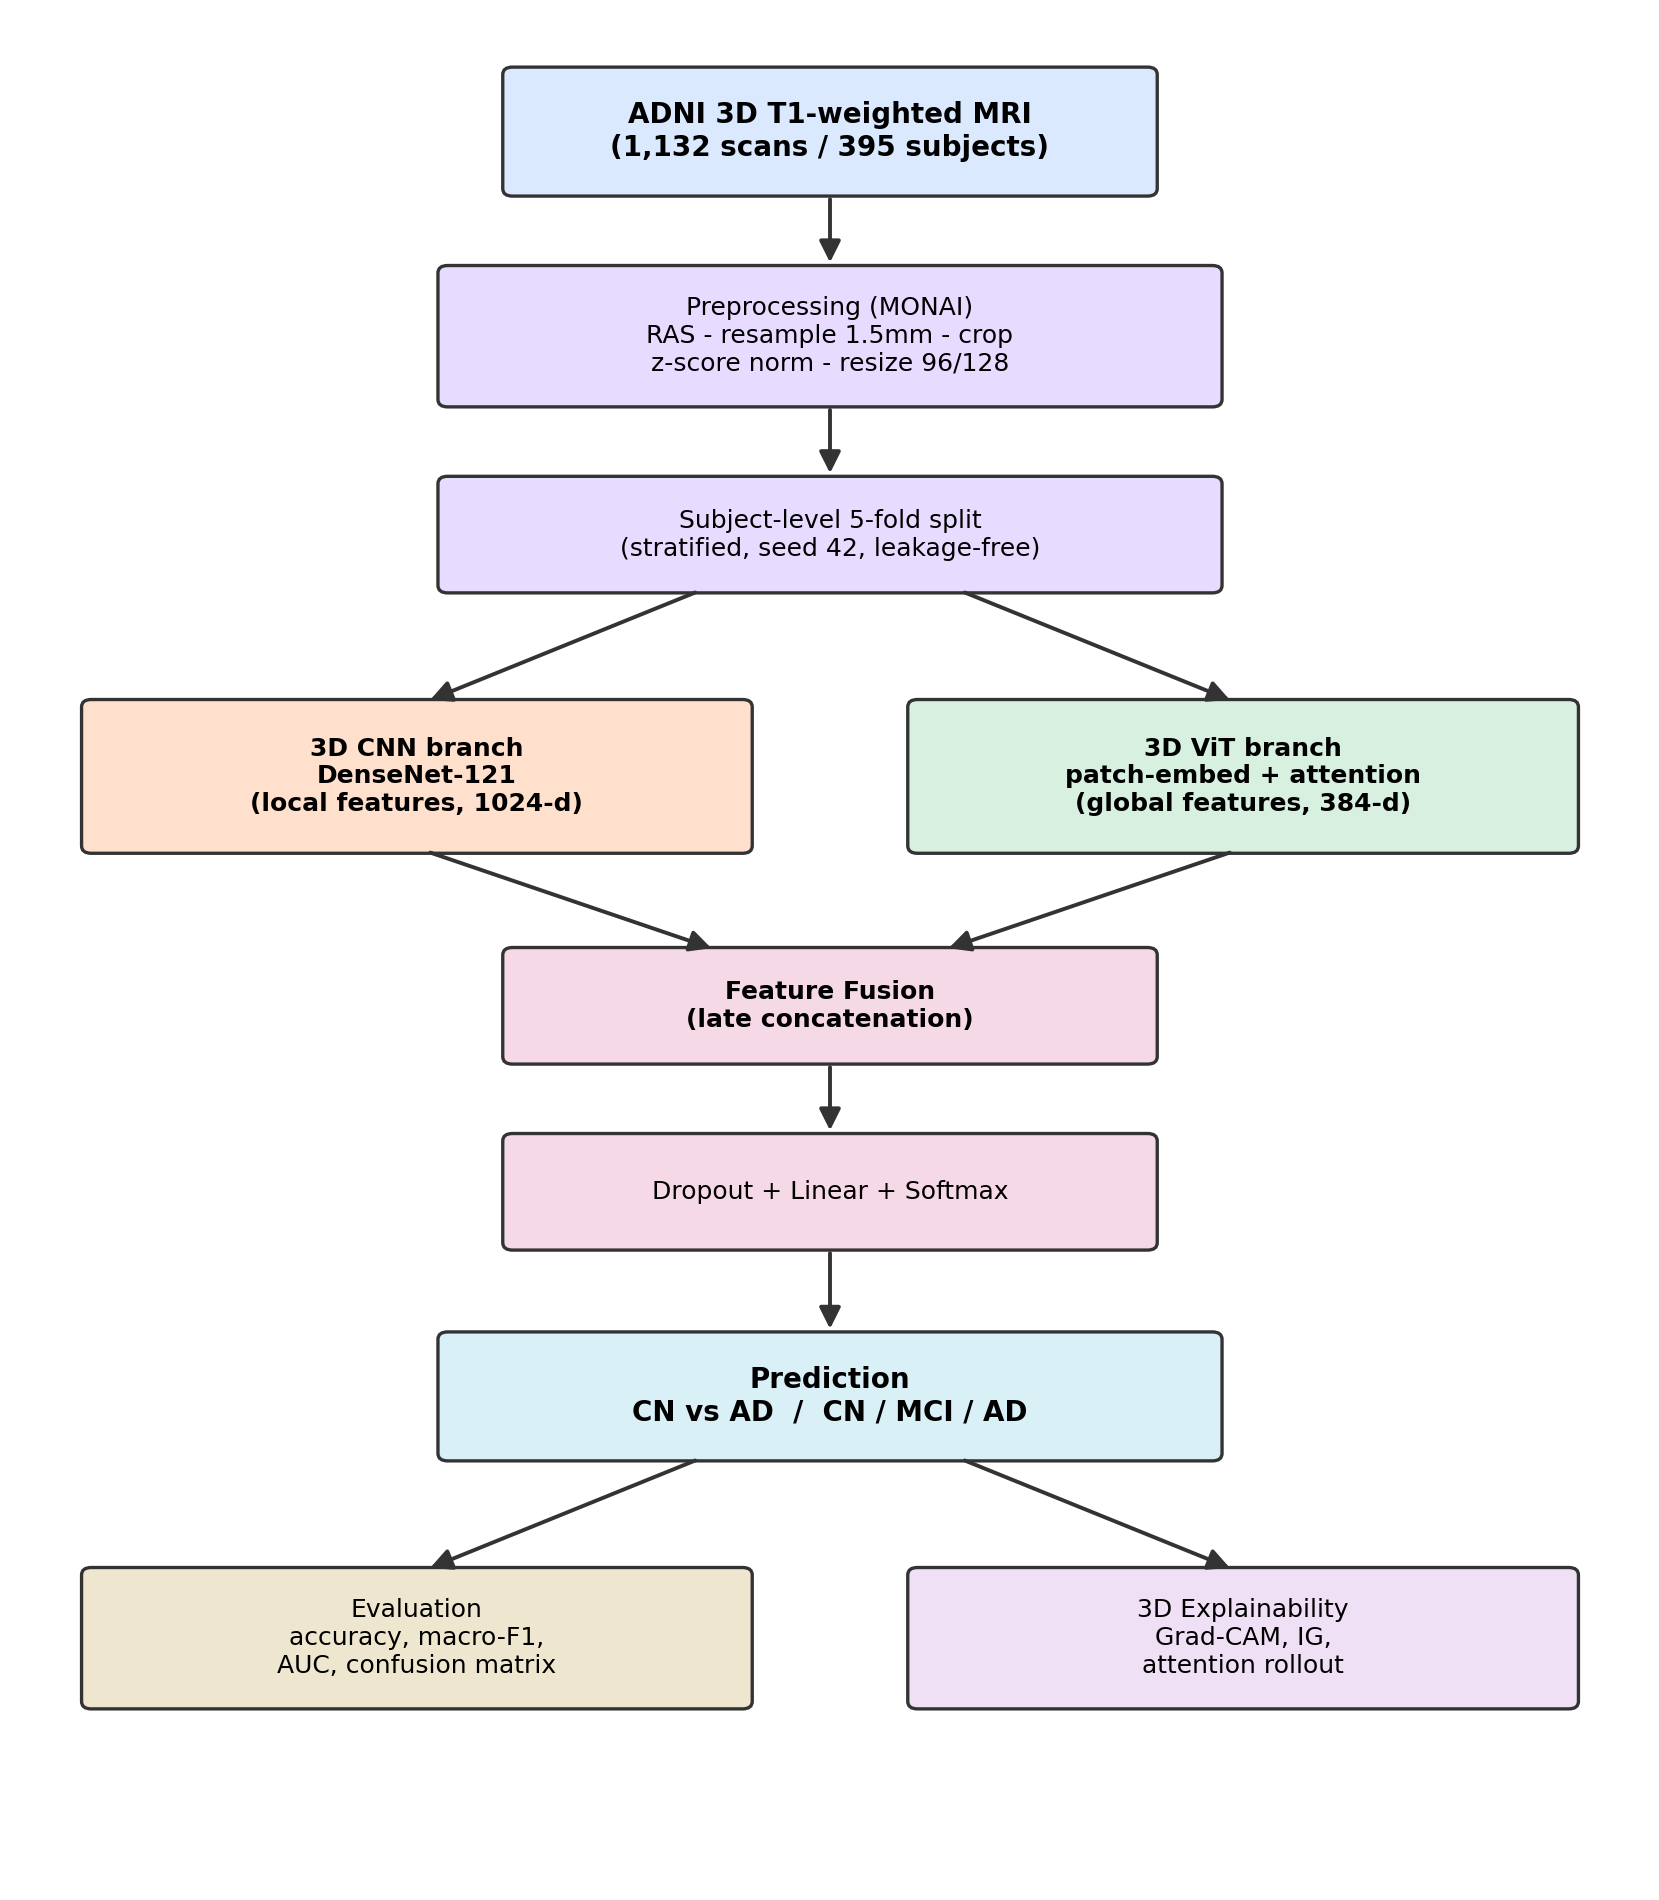
\includegraphics[width=11cm]{Images/arch_block_diagram.png}
    \caption[System block diagram]{\textbf{System block diagram.} High-level view of the proposed dual-branch 3D CNN--ViT system on ADNI.}
    \label{fig:block}
\end{figure}
\begin{figure}[H]
    \centering
    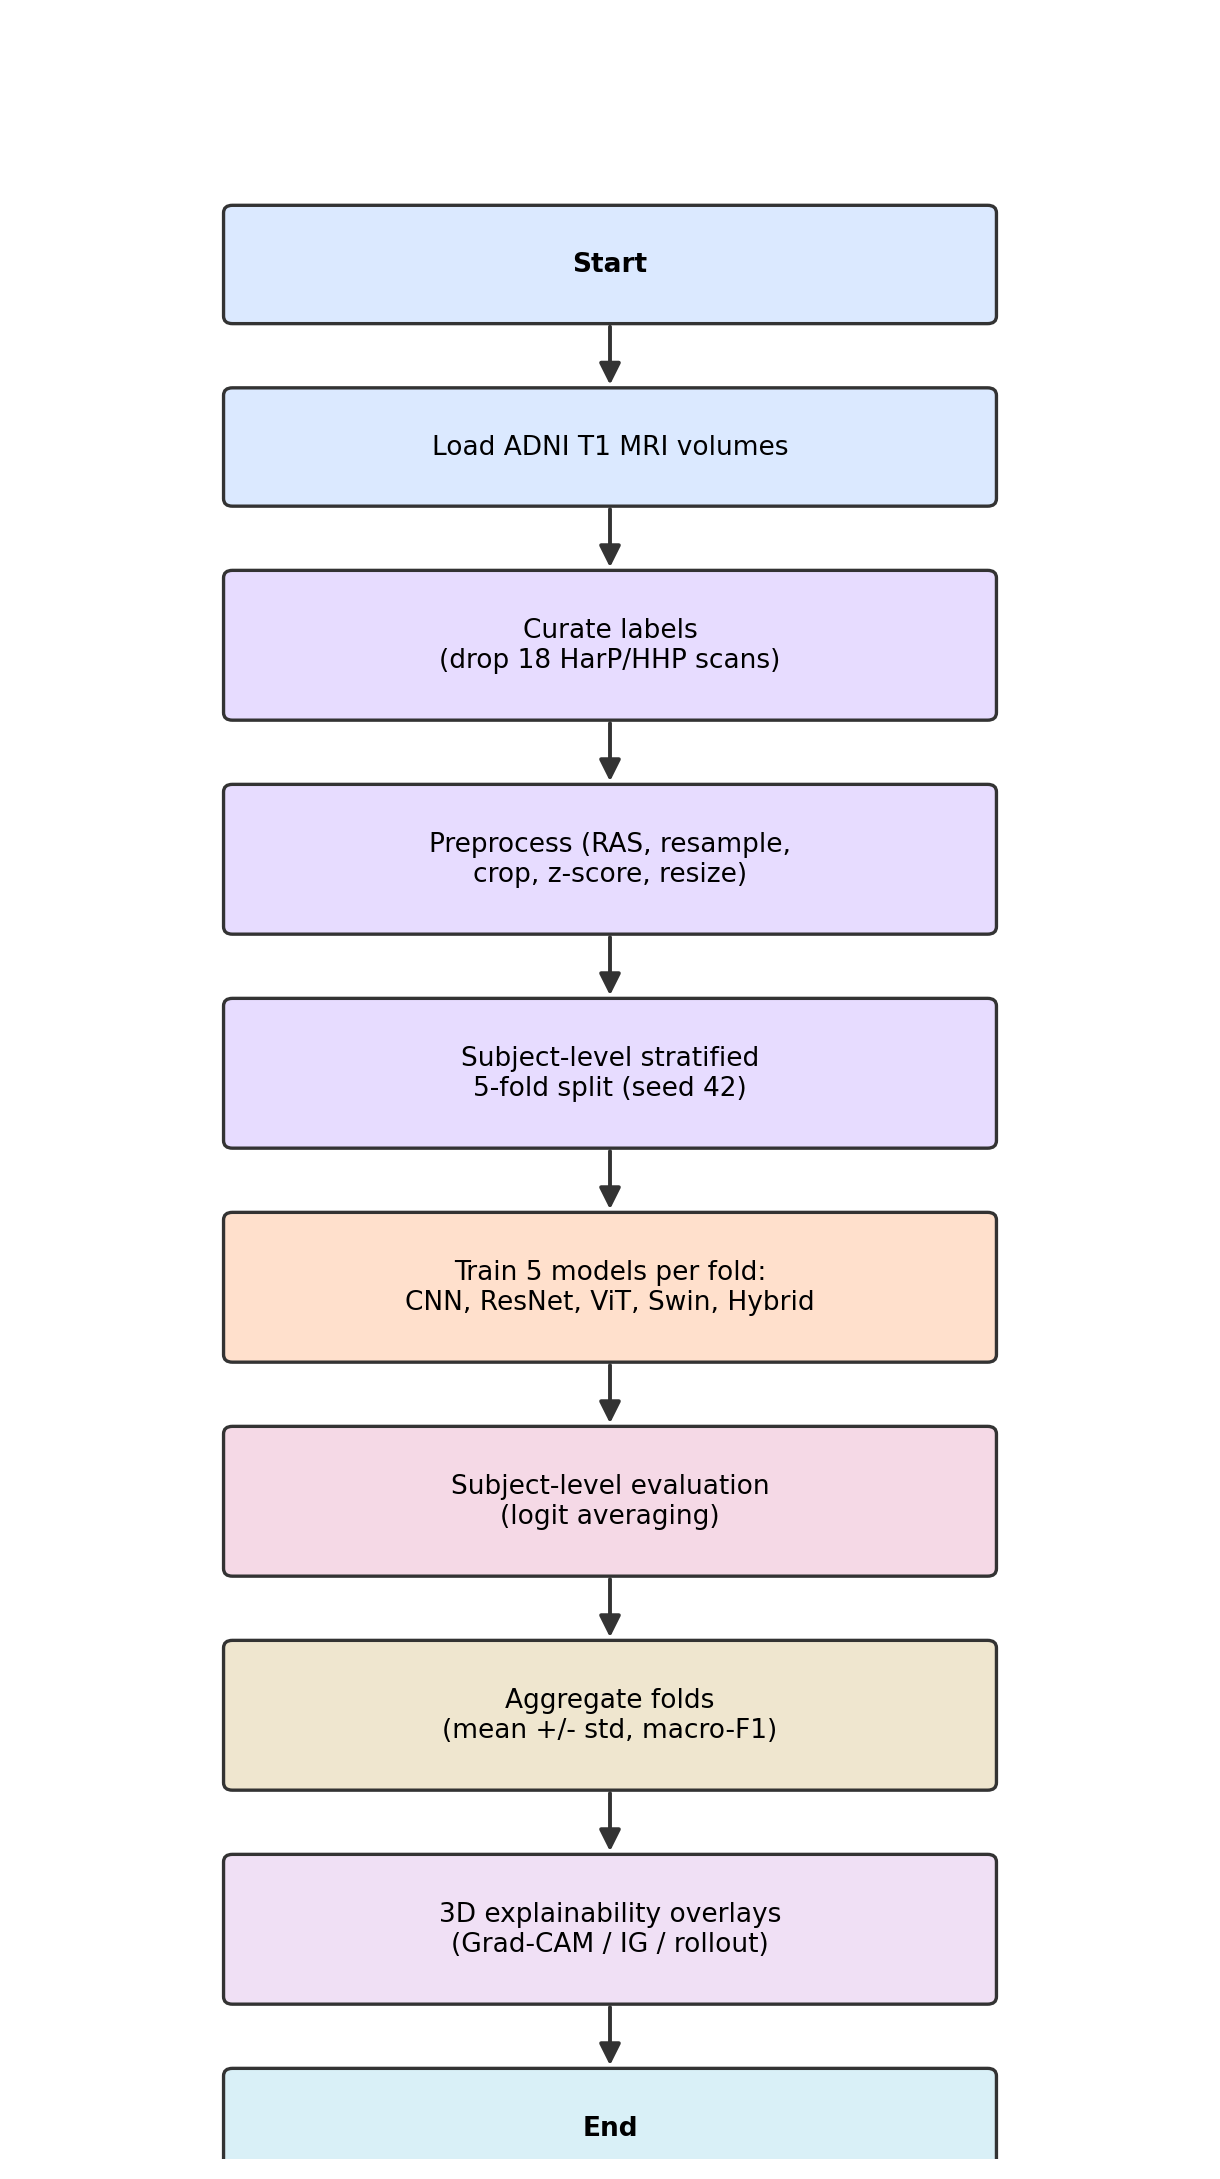
\includegraphics[width=9cm]{Images/arch_flowchart.png}
    \caption[Experimental flowchart]{\textbf{Experimental flowchart.} End-to-end pipeline from ADNI ingestion to subject-level evaluation and explainability.}
    \label{fig:flow}
\end{figure}
\begin{figure}[H]
    \centering
    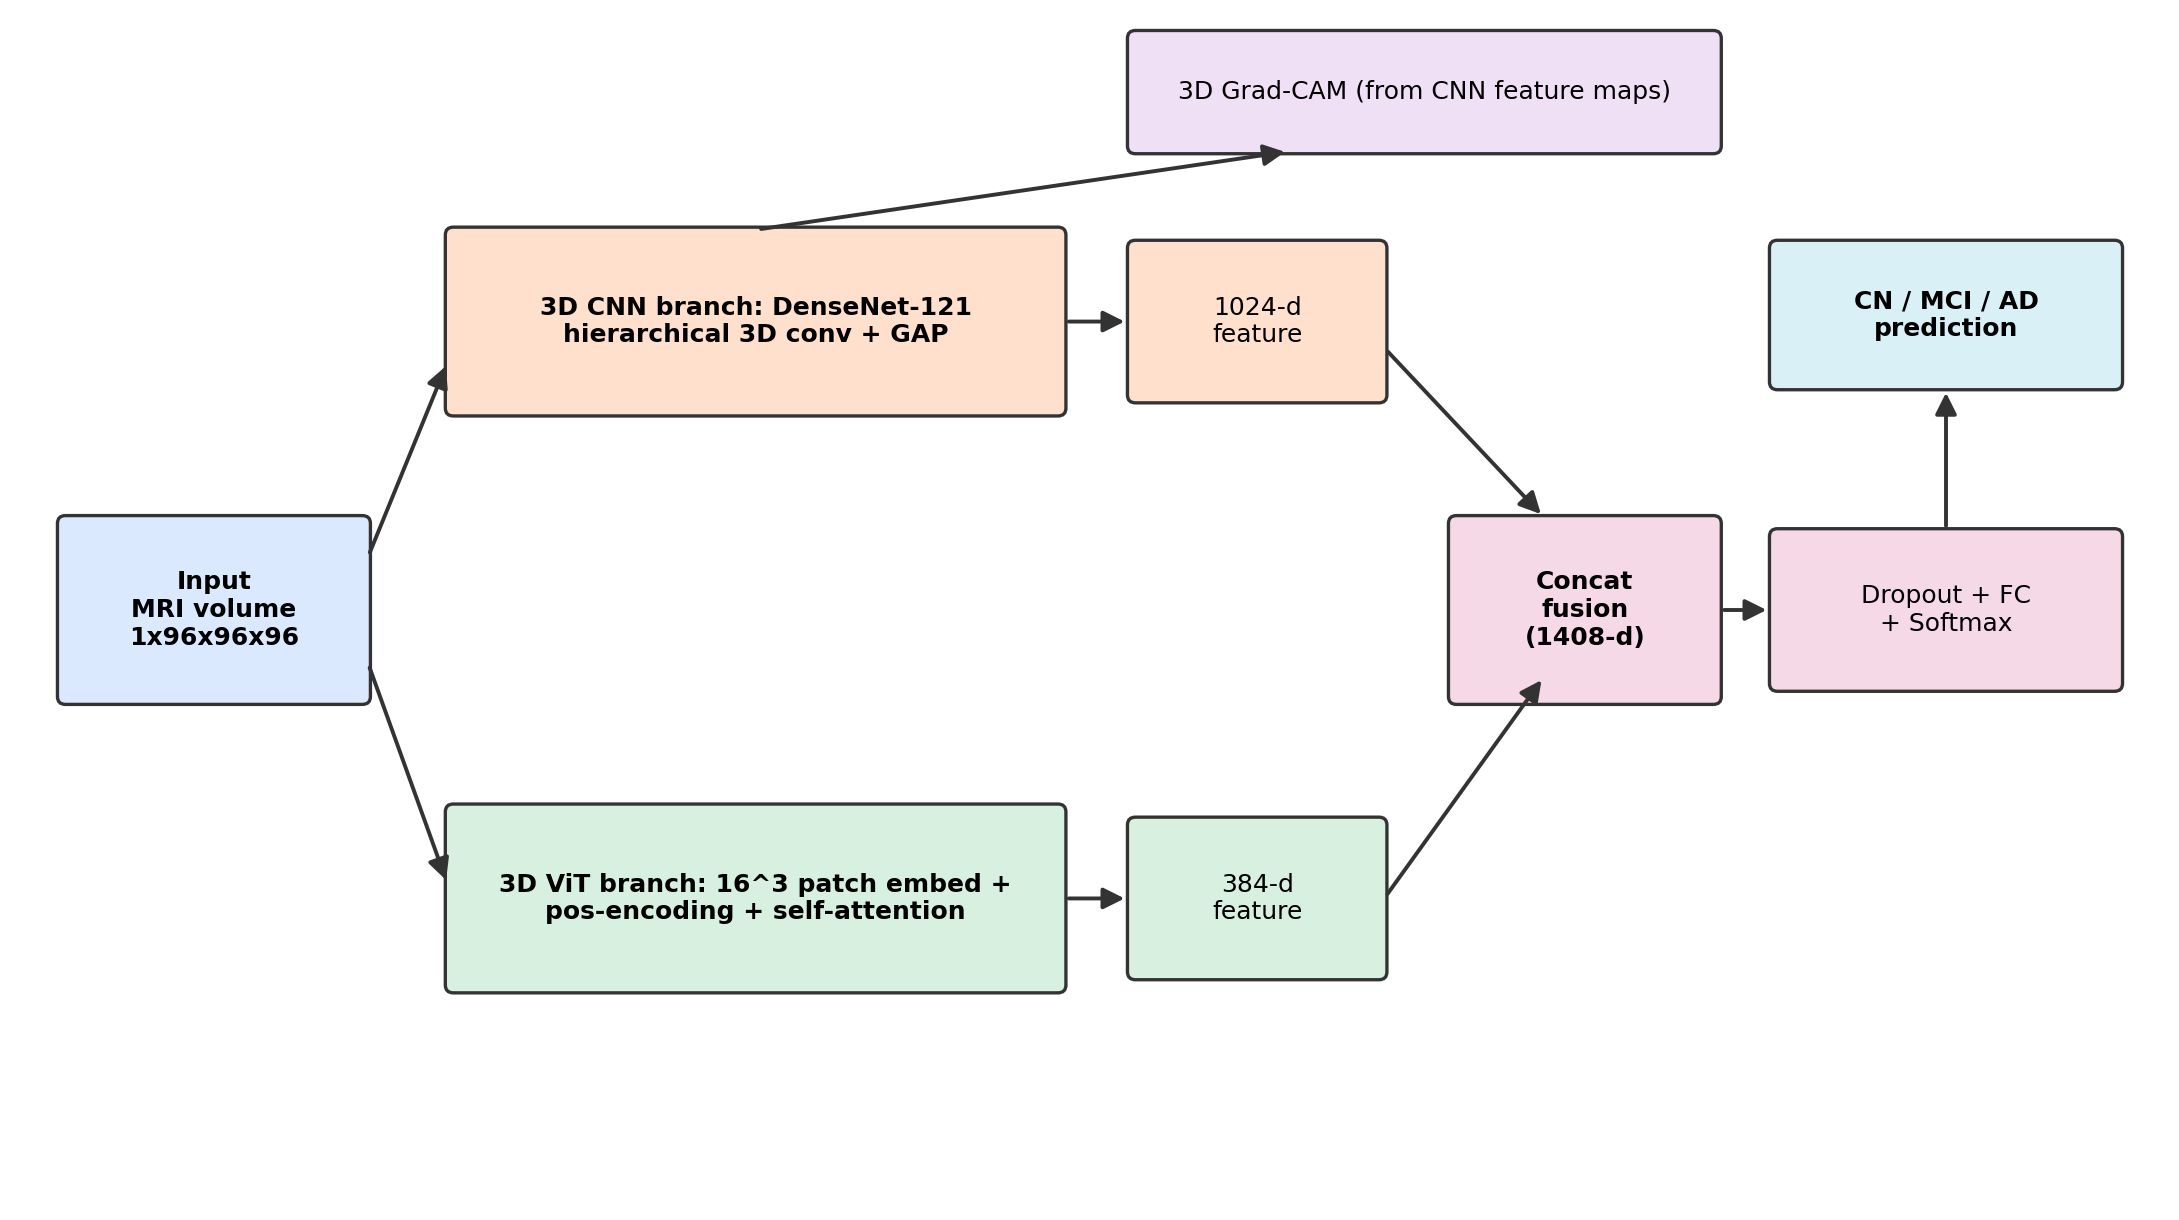
\includegraphics[width=15cm]{Images/arch_hybrid.png}
    \caption[Hybrid fusion architecture]{\textbf{Hybrid fusion architecture.} The 3D CNN (DenseNet) branch extracts local texture features (1024-D) and the 3D ViT branch extracts global contextual features (384-D) from the \emph{same} input volume; the two vectors are combined by late concatenation (1408-D) and passed to a shared dropout$+$linear classifier head with softmax. Grad-CAM is computed from the CNN branch for explainability.}
    \label{fig:hybrid}
\end{figure}

\subsection{Design Alternatives and Rationale}
Several architectural alternatives were considered. A standalone 3D CNN captures local spatial features strongly but has a limited receptive field for long-range relationships. A standalone 3D Vision Transformer models global context well but is data-hungry and, as the experiments confirm, underperforms when trained from scratch on a few hundred subjects. A 2D slice-based model is easy and fast but discards volumetric context and, worse, invites patient-level data leakage.\\
Weighing performance potential, resource cost, and --- crucially --- evaluation honesty, the hybrid 3D CNN--3D ViT architecture was selected: the CNN branch supplies fine local anatomical detail and the inductive bias the transformer lacks, while the ViT branch adds global reasoning across the whole volume. Fusing the two, combined with 3D Grad-CAM, yields a design that is modular, efficient on a single 16\,GB GPU, and --- as Chapter~\ref{cha:results} shows --- statistically tied for the best binary result with the standalone CNN, which is itself an informative outcome of a fair comparison against its own single-model baselines.

\section{Pseudocode for Proposed 3D CNN--ViT Hybrid Model}
\begin{algorithm}[H]
\caption{Hybrid 3D CNN--ViT Classification Pipeline}
\begin{algorithmic}[1]
\Require MRI\_volume (Raw 3D Brain Scan)
\Ensure Prediction $\in$ \{CN, AD\} (binary) or \{CN, MCI, AD\} (three-class)

\State MRI $\gets$ LoadVolume(MRI\_volume)
\State MRI $\gets$ Preprocess(MRI)
\Statex \quad ReorientRAS();\ ResampleIsotropic();\ CropForeground()
\Statex \quad ZScoreNormalize();\ Resize()
\Statex \quad \textit{// skull-stripping / MNI registration optional (ablation)}
\State Volume $\gets$ Standardize(MRI)

\State CNN\_features $\gets$ DenseNet3D(Volume) \Comment{local, 1024-d}
\State ViT\_features $\gets$ ViT3D(Volume) \Comment{global, 384-d}

\State Fused $\gets$ Concatenate(CNN\_features, ViT\_features)
\State Output $\gets$ FullyConnected(Dropout(Fused))
\State Prediction $\gets$ Softmax(Output)

\State Heatmap $\gets$ GradCAM3D(CNN\_features)
\State \textbf{return} Prediction, Heatmap
\end{algorithmic}
\end{algorithm}

\section{Summary}
This chapter presented the system design underlying the proposed framework. It specified the stakeholders, functional and non-functional requirements (including the explicit requirement of an \emph{honest}, subject-level accuracy target), and a five-module architecture spanning data curation, 3D preprocessing, the CNN/ViT/Swin/hybrid feature-extraction bank, explainability, and evaluation. The block, flowchart, and hybrid-architecture diagrams illustrated component interaction and data flow, and the pseudocode clarified the operational path from a raw MRI volume to a classified, explained prediction. This blueprint guides the methodology and experiments that follow.


\chapter{Methodology and Implementation}
\label{cha:MethodologyAndImplementationU}
This chapter presents the methodological framework, tools, data pipeline, model design, and training protocol used to build and benchmark the proposed Alzheimer's Disease (AD) detection system. The emphasis is on \emph{how} a family of fully three-dimensional models --- a 3D CNN, a pretrained 3D ResNet, a 3D Vision Transformer (ViT), a Swin Transformer, and a hybrid 3D CNN--ViT --- was developed, trained, and evaluated on identical data and splits, so that the single-vs-hybrid comparison at the heart of this thesis is fair and reproducible.

\section{Methodological Framework}
The methodology was structured into sequential stages to ensure a systematic and leakage-free implementation. The workflow began with \textbf{problem formulation}: rather than chasing a single inflated accuracy figure, the goal was fixed as an \emph{honest, subject-level} comparison of 3D deep-learning architectures on structural MRI. Two clinically meaningful classification tasks were defined:
\begin{enumerate}
    \item \textbf{Binary CN-vs-AD} --- separating cognitively normal (CN) subjects from Alzheimer's (AD) subjects. This is the headline task, where high accuracy is genuinely achievable.
    \item \textbf{Three-class CN/MCI/AD} --- additionally distinguishing mild cognitive impairment (MCI), the transitional stage. This is reported as the harder, honest benchmark.
\end{enumerate}
\textbf{Data acquisition} used a single, authoritative source, the Alzheimer's Disease Neuroimaging Initiative (ADNI), to avoid the domain-shift and label-mismatch problems that arise when 2D and 3D datasets are mixed. \textbf{Preprocessing and data preparation} standardized every volume into a common orientation, resolution, and intensity range using MONAI transforms. In the \textbf{modelling} stage, five architectures sharing a common feature-extraction interface and classifier head were built. \textbf{Training and evaluation} were performed with five-fold subject-level cross-validation, reporting mean $\pm$ standard deviation across folds. Finally, \textbf{explainability} was applied with a suite of 3D attribution methods to verify that the models attend to anatomically plausible regions.

\begin{figure}[H]
    \centering
    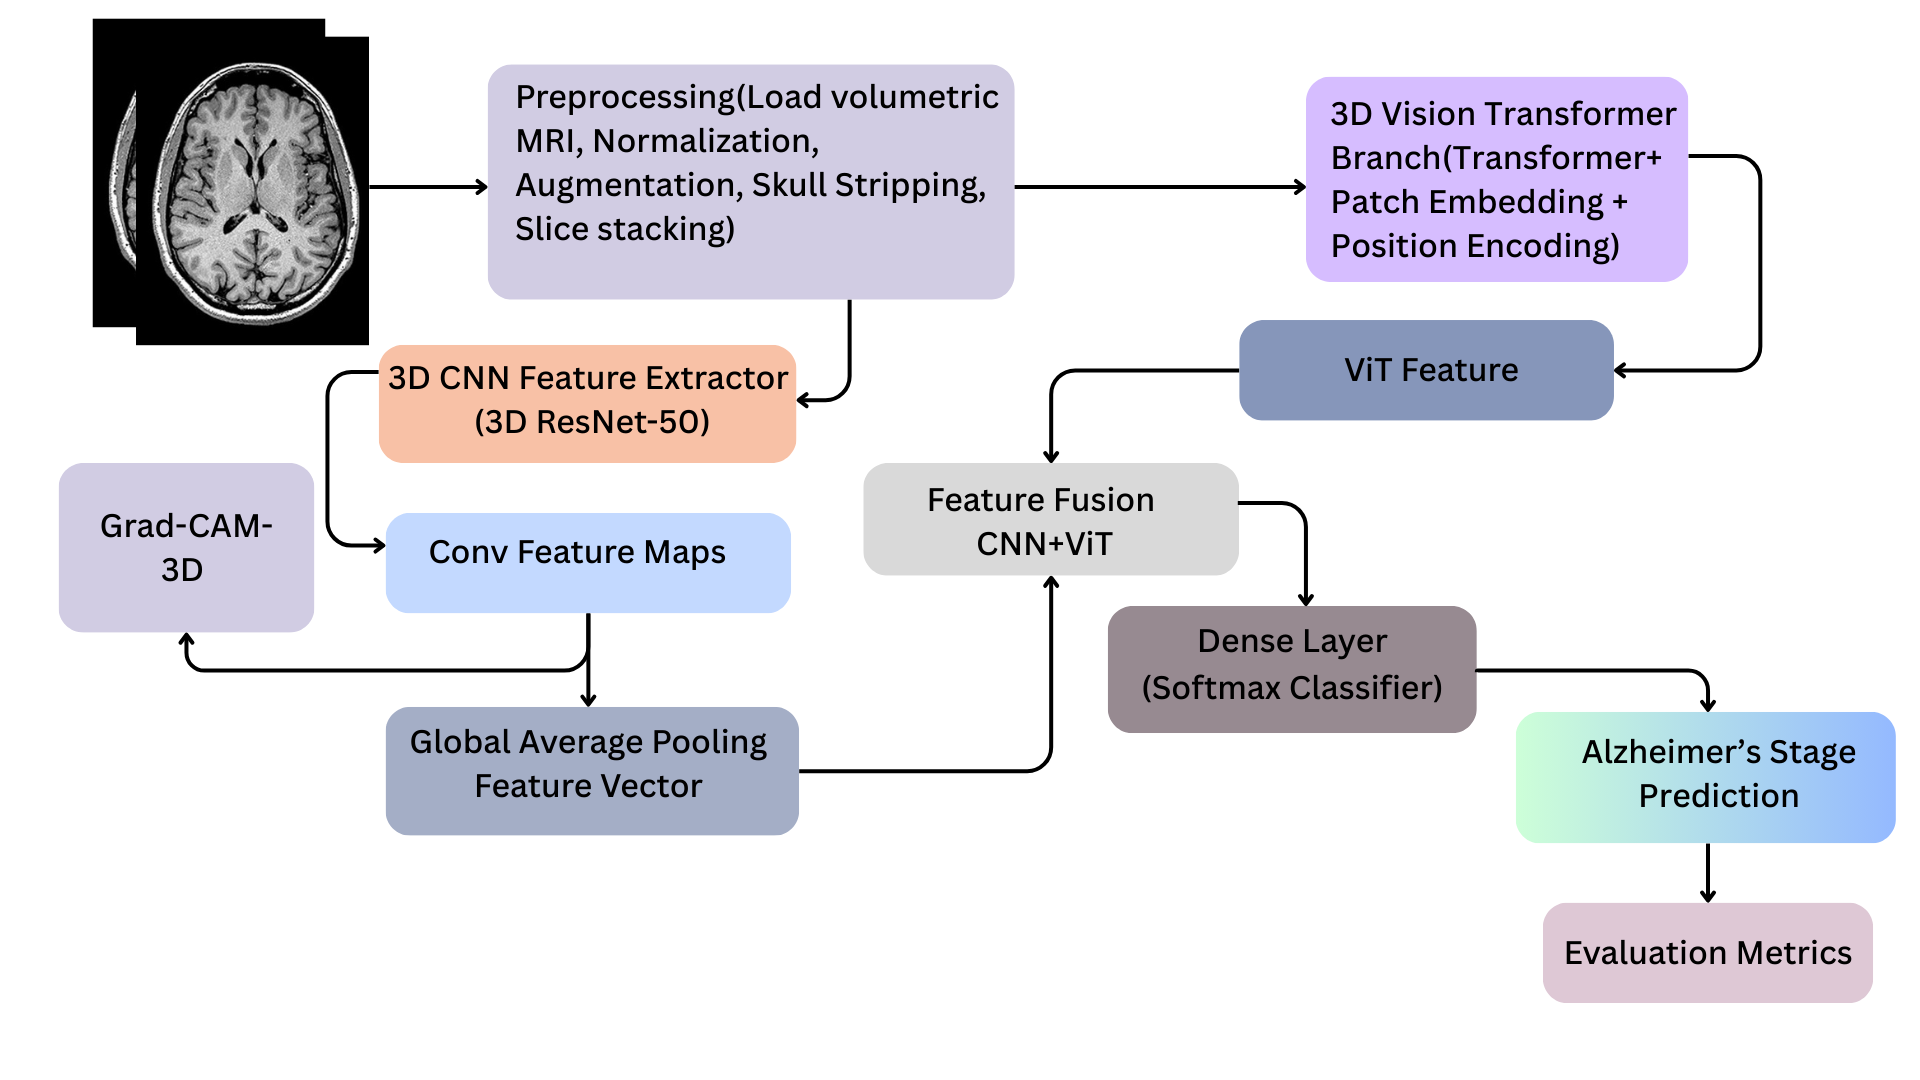
\includegraphics[width=15cm]{Images/Methodology_diagram.png}
    \caption[Methodology overview]{\textbf{Methodology overview.} End-to-end study workflow: problem formulation, single-source ADNI acquisition, deterministic MONAI preprocessing, five 3D architectures sharing a common classifier head, subject-level five-fold training and evaluation reported as mean\,$\pm$\,std, and 3D explainability.}
    \label{fig:methodology}
\end{figure}

\section{Tools, Libraries, and Technologies Used}
The system was implemented entirely in Python using the PyTorch + MONAI stack for 3D medical imaging. The primary tools are:\\
\textbf{Programming Language}: Python 3.10.\\
\textbf{Deep Learning Frameworks}:
\begin{enumerate}
    \item PyTorch 2.11 (CUDA 12.8)~\cite{paszke2019pytorch} --- 3D model implementation, mixed-precision training loops, GPU optimization.
    \item MONAI 1.6~\cite{cardoso2022monai} --- medical-imaging transforms, cached datasets, and the 3D backbone implementations (DenseNet121, ResNet, ViT, SwinUNETR encoder).
\end{enumerate}
\textbf{Supporting Libraries}:\\
NumPy 1.26, SciPy --- numerical operations.\\
NiBabel 5.4 --- reading NIfTI (.nii) MRI volumes.\\
scikit-learn 1.4 --- evaluation metrics (F1, ROC-AUC, confusion matrices) and cross-validation utilities.\\
Matplotlib, Seaborn, scikit-image --- visualization and explainability overlays.\\
TensorBoard --- per-run training curves; results also logged to CSV/JSON.\\
\textbf{Development Environment}: local workstation with VS Code; experiments are fully config-driven (one YAML per run) for reproducibility.\\
\textbf{Hardware}: a single NVIDIA GeForce RTX 5060 Ti (16 GB VRAM), 32 GB system RAM, SSD storage. The 16 GB VRAM budget is the binding constraint that drives several design choices below (input resolution, batch size, gradient accumulation).

\section{Dataset Description}
This study uses the \textbf{ADNI} dataset~\cite{jack2008adni,petersen2010adni} exclusively (ADNI GO/2/3, 3T, 3D T1-weighted MPRAGE, pre-processed N3m NIfTI volumes). Using a single, curated source --- rather than pooling ADNI with slice-based datasets such as MIRIAD or Kaggle --- keeps the labels, modality, and acquisition consistent and makes the subject-level split enforceable.

\subsection{ADNI (Alzheimer's Disease Neuroimaging Initiative)}
ADNI is one of the most widely used and authoritative neuroimaging resources for dementia research, providing T1-weighted 3D MRI collected across multiple sites, scanners, and longitudinal timepoints.\\
Source: ADNI (adni.loni.usc.edu)\\
Scan Type: 3D T1-weighted MPRAGE (GradWarp, N3m corrected)\\
Diagnostic groups used: CN, MCI, AD\\
Field strength: 3T\\
Native resolution: $\sim$256$\times$256$\times$170 voxels ($\sim$1\,mm isotropic)\\
Attributes: subject ID, group, sex, age, acquisition description.

\subsection{Curation and Class Distribution}
The raw export was cleaned to one row per usable scan. \textbf{18 scans (from 9 subjects) were removed}: the \textit{HarP 135} files are hippocampus \emph{segmentations} rather than whole-brain MRI, and the \textit{HHP AC-PC registered} files follow an off-pipeline protocol; those 9 subjects retain their standard N3m scans, so no subject is lost. The curated cohort is summarized in Table~\ref{tab:dataset}.

\begin{table}[H]
\centering
\caption{ADNI cohort after curation (subject-level and scan-level counts).}
\label{tab:dataset}
\begin{tabular}{|l|c|c|c|c|}
\hline
\textbf{Group} & \textbf{Subjects} & \textbf{Scans} & \textbf{Binary task} & \textbf{3-class task} \\
\hline
CN (Cognitively Normal) & 206 & 627 & \checkmark & \checkmark \\
MCI (Mild Cognitive Impairment) & 80 & 182 & --- & \checkmark \\
AD (Alzheimer's Disease) & 109 & 323 & \checkmark & \checkmark \\
\hline
\textbf{Total (3-class)} & \textbf{395} & \textbf{1{,}132} & & \checkmark \\
\textbf{Total (binary, CN+AD)} & \textbf{315} & \textbf{950} & \checkmark & \\
\hline
\end{tabular}
\end{table}

The dataset is \emph{imbalanced} (CN is the majority; MCI is the minority at only 80 subjects), which motivates the use of class-weighted / focal loss and macro-F1 as the primary metric. Several subjects contribute multiple longitudinal scans, which makes the subject-level split (below) essential. Each scan inherits its subject's diagnostic group. \authortodo{confirm whether the group is the baseline (screening) diagnosis or the diagnosis at each visit, and report the follow-up span. If baseline labels are used, a CN or MCI subject who converted at a later visit keeps the old label on later scans, which adds label noise. Also confirm whether the 180 subjects with exactly four scans have four visits, or repeat acquisitions (MPRAGE and MPRAGE-repeat) within fewer sessions.}

\subsection{Exploratory Data Analysis}
Figure~\ref{fig:ds_stats} summarizes the cohort: the class balance (per subject and per scan), the age and sex distributions, and the number of scans per subject. The distributions confirm the expected demographics of an AD cohort (older, with a mild sex skew) and the strong CN/AD-vs-MCI imbalance. AD subjects are on average older than CN subjects (the age densities peak at roughly 76 and 70 years respectively), so age is a potential confounder of atrophy-based classification; this is discussed under Threats to Validity in Chapter~\ref{cha:results}. Figure~\ref{fig:ds_samples} shows representative axial, coronal, and sagittal slices of a CN and an AD subject; the enlarged ventricles and reduced medial-temporal volume in the AD example are visible even to the eye, and are precisely the structural cues the models are expected to learn.

\begin{figure}[H]
    \centering
    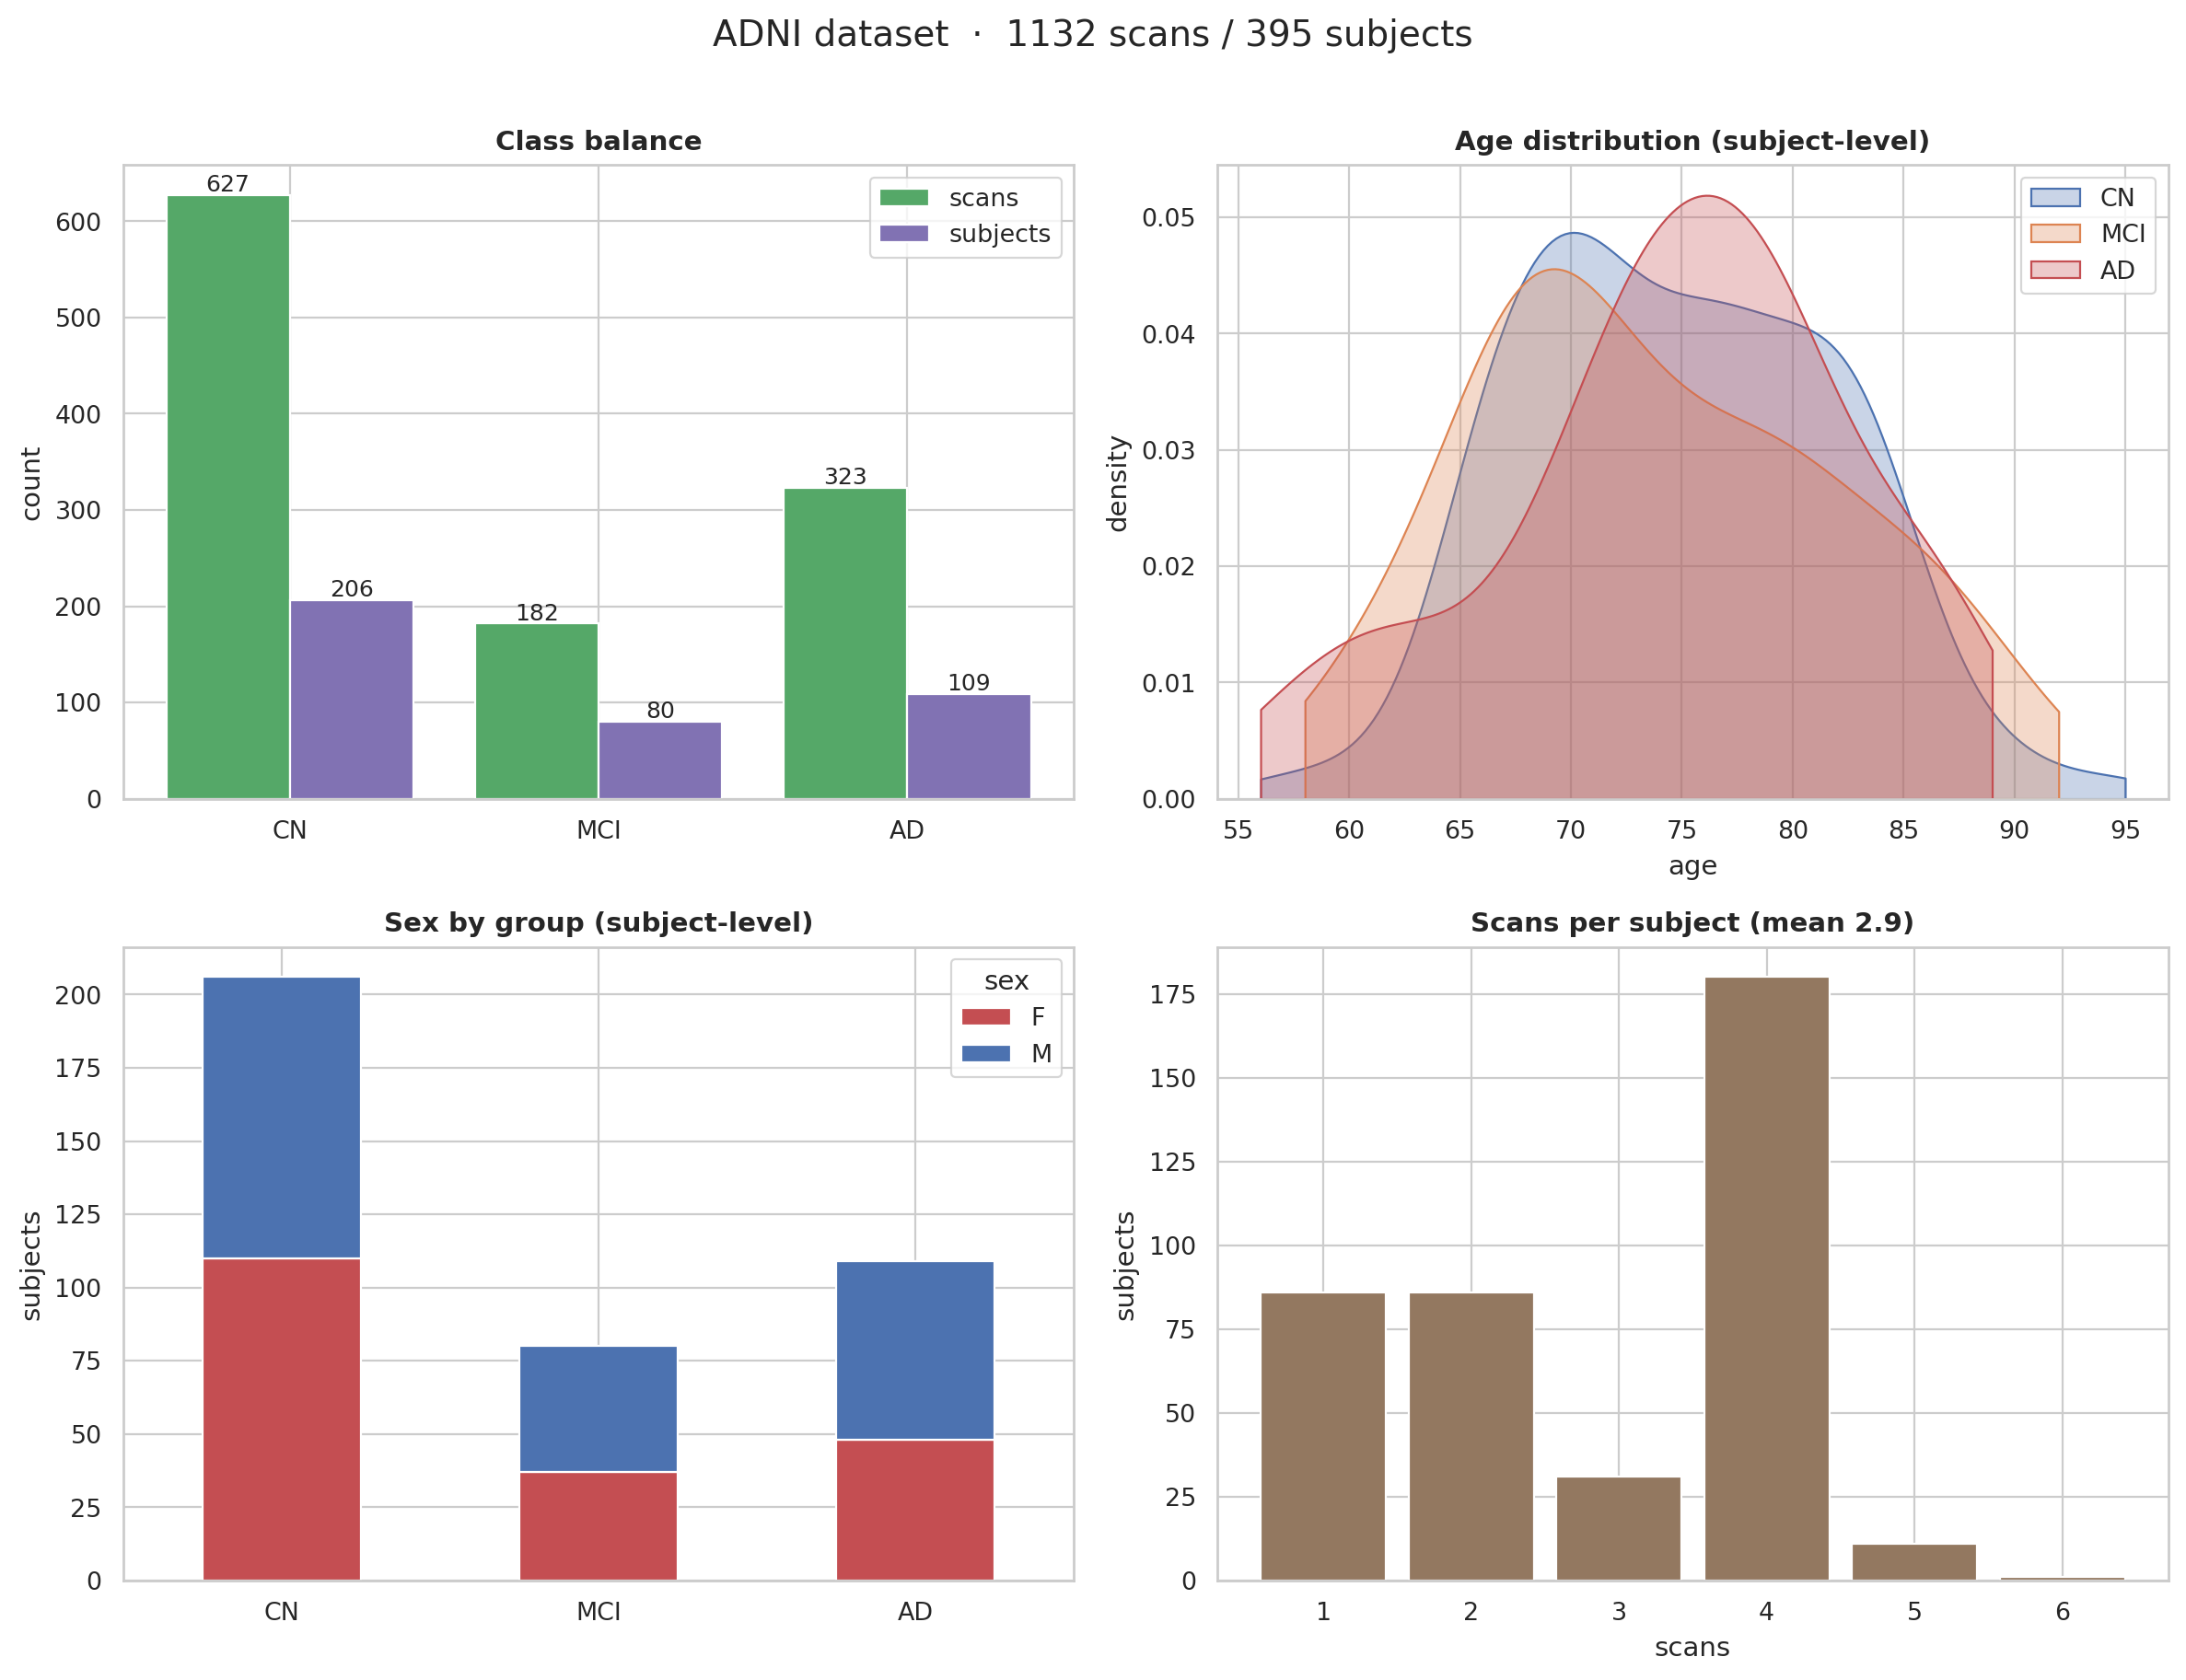
\includegraphics[width=15cm]{Images/ds_stats.png}
    \caption[Cohort statistics]{\textbf{Cohort statistics.} ADNI class balance, age/sex demographics, and scans per subject.}
    \label{fig:ds_stats}
\end{figure}

\begin{figure}[H]
    \centering
    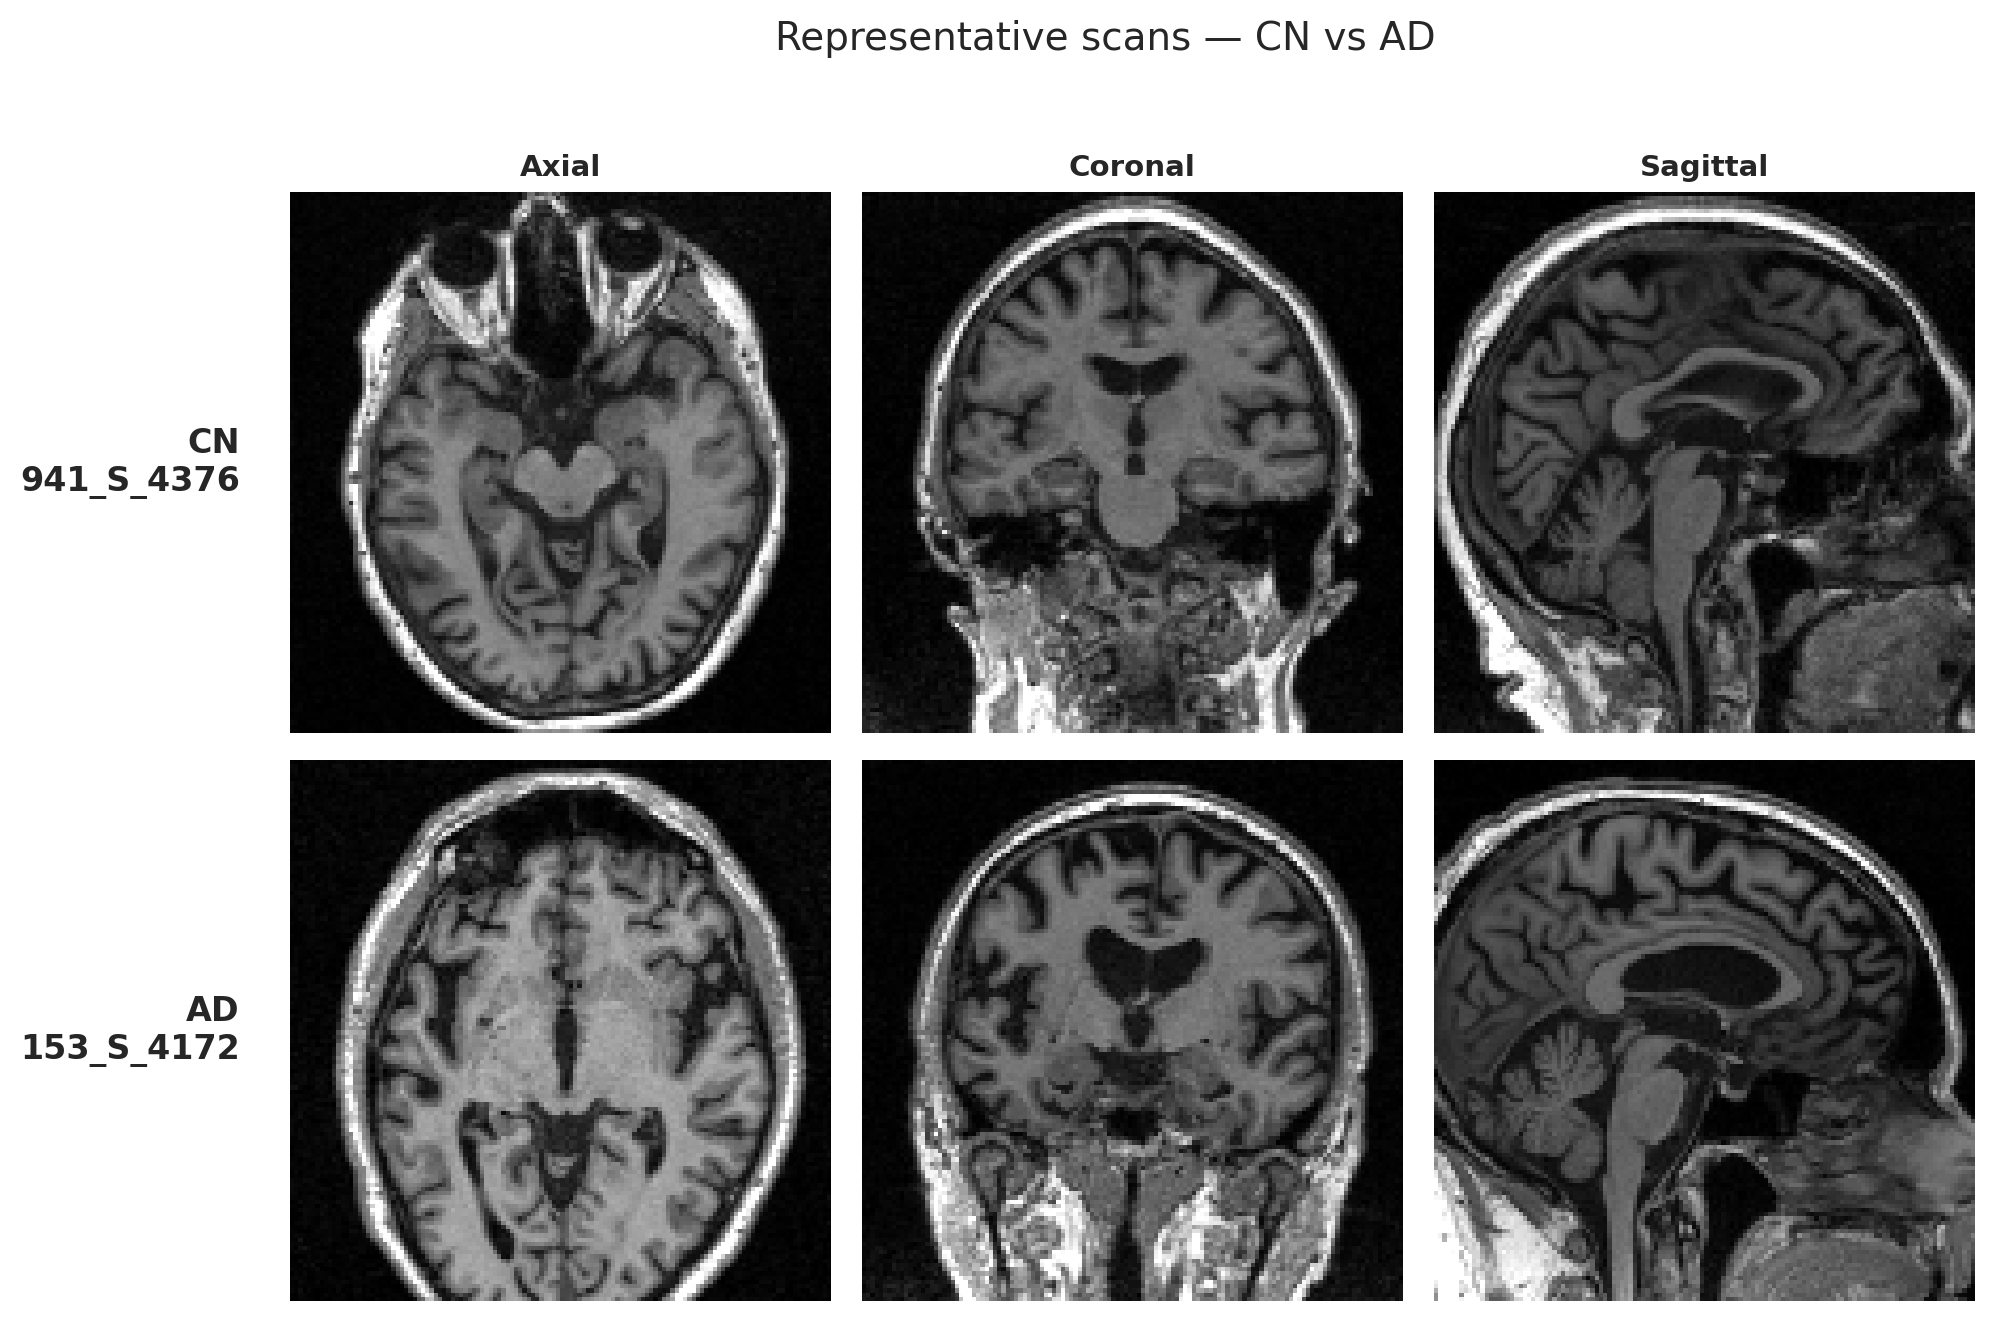
\includegraphics[width=14cm]{Images/ds_samples.png}
    \caption[CN vs.\ AD samples]{\textbf{CN vs.\ AD samples.} Representative preprocessed volumes of a cognitively normal (CN) and an Alzheimer's (AD) subject across the three anatomical planes.}
    \label{fig:ds_samples}
\end{figure}

\subsection{Evaluation Protocol (Subject-Level, Leakage-Free)}
The single most important methodological decision is that \textbf{no subject's scans are ever split across training and testing}. This is enforced and asserted in code (\texttt{build\_dataset.py}). Concretely:
\begin{itemize}
    \item \textbf{Subject-level stratified 5-fold cross-validation} is the primary protocol; a 70/15/15 subject-level hold-out split is also provided. Both use \texttt{seed = 42} and are identical for every model, so comparisons are fair.
    \item \textbf{Two-level metrics.} Each scan is scored (scan-level); in addition, the softmax logits of a subject's multiple scans are averaged into one subject-level prediction --- the clinically meaningful number, and a legitimate, leakage-free boost of a few points.
    \item \textbf{Metrics.} Accuracy, \textbf{macro-F1 (primary, due to imbalance)}, weighted-F1, per-class precision/recall/F1, confusion matrices, and ROC-AUC (one-vs-rest for the three-class task).
    \item \textbf{Model selection / early stopping} is on validation subject-level macro-F1, never on accuracy. \authortodo{state exactly which subjects form the validation set inside each fold. If the held-out test fold itself was used for early stopping, say so here and in the Threats to Validity, because selecting the best epoch on the test fold biases the reported scores upward; the preferred fix is an inner validation split carved from the four training folds.}
    \item \textbf{Reference baseline.} Every table is read against the majority-class baseline --- always predicting CN --- which scores $206/315 = 65.4\%$ accuracy on the binary task and $206/395 = 52.2\%$ on the three-class task. Accuracy is only meaningful in excess of these figures, which is a further reason for using macro-F1.
\end{itemize}
This protocol is deliberately conservative: it produces lower numbers than slice-level splitting, but numbers that would survive scrutiny on unseen patients~\cite{wen2020convolutional,yagis2021effect}.

\section{Preprocessing Steps}
A single deterministic MONAI pipeline is applied identically to train, validation, and test volumes (augmentation is train-only). Steps:\\
\textbf{Load \& channel-first:} read NIfTI, add a channel dimension.\\
\textbf{Orientation:} reorient to canonical RAS axes.\\
\textbf{Resampling:} resample to 1.5\,mm isotropic spacing for a consistent physical scale.\\
\textbf{Foreground crop:} \texttt{CropForeground} removes empty background around the head.\\
\textbf{Intensity normalization:} per-volume z-score normalization over non-zero voxels.\\
\textbf{Resize / pad:} to a fixed cubic tensor --- $96^3$ for every binary run and for the three-class ViT, and $128^3$ for the three-class CNN and Swin (Appendix~\ref{app:repro}); the transformer patch-embedding and the 16\,GB VRAM budget make $96^3$ the practical size for the hybrids.\\
\textbf{Caching:} a MONAI \texttt{CacheDataset} computes this deterministic pipeline once and reuses it, giving a large speed-up on the small cohort.\\[4pt]
\textbf{Note on skull-stripping.} The ADNI N3m volumes are \emph{not} skull-stripped, and this pipeline does not strip them by default; brain extraction and MNI registration are treated as optional ablations rather than a fixed step. This is stated explicitly because it affects how the explainability maps in Chapter~\ref{cha:results} are interpreted (importance is reported over coarse spatial regions of the head volume, not atlas ROIs).\\[4pt]
\textbf{Data Augmentation (train only):} random flips, random affine ($\pm10^{\circ}$ rotation, mild scaling/translation), Gaussian noise and smoothing, random bias field, gamma/contrast adjustment, and intensity scale/shift. These act as strong regularizers on a small dataset.

Figure~\ref{fig:preproc} illustrates the deterministic preprocessing pipeline applied to every volume, and Figure~\ref{fig:augment} shows examples of the stochastic training-time augmentations.

\begin{figure}[H]
    \centering
    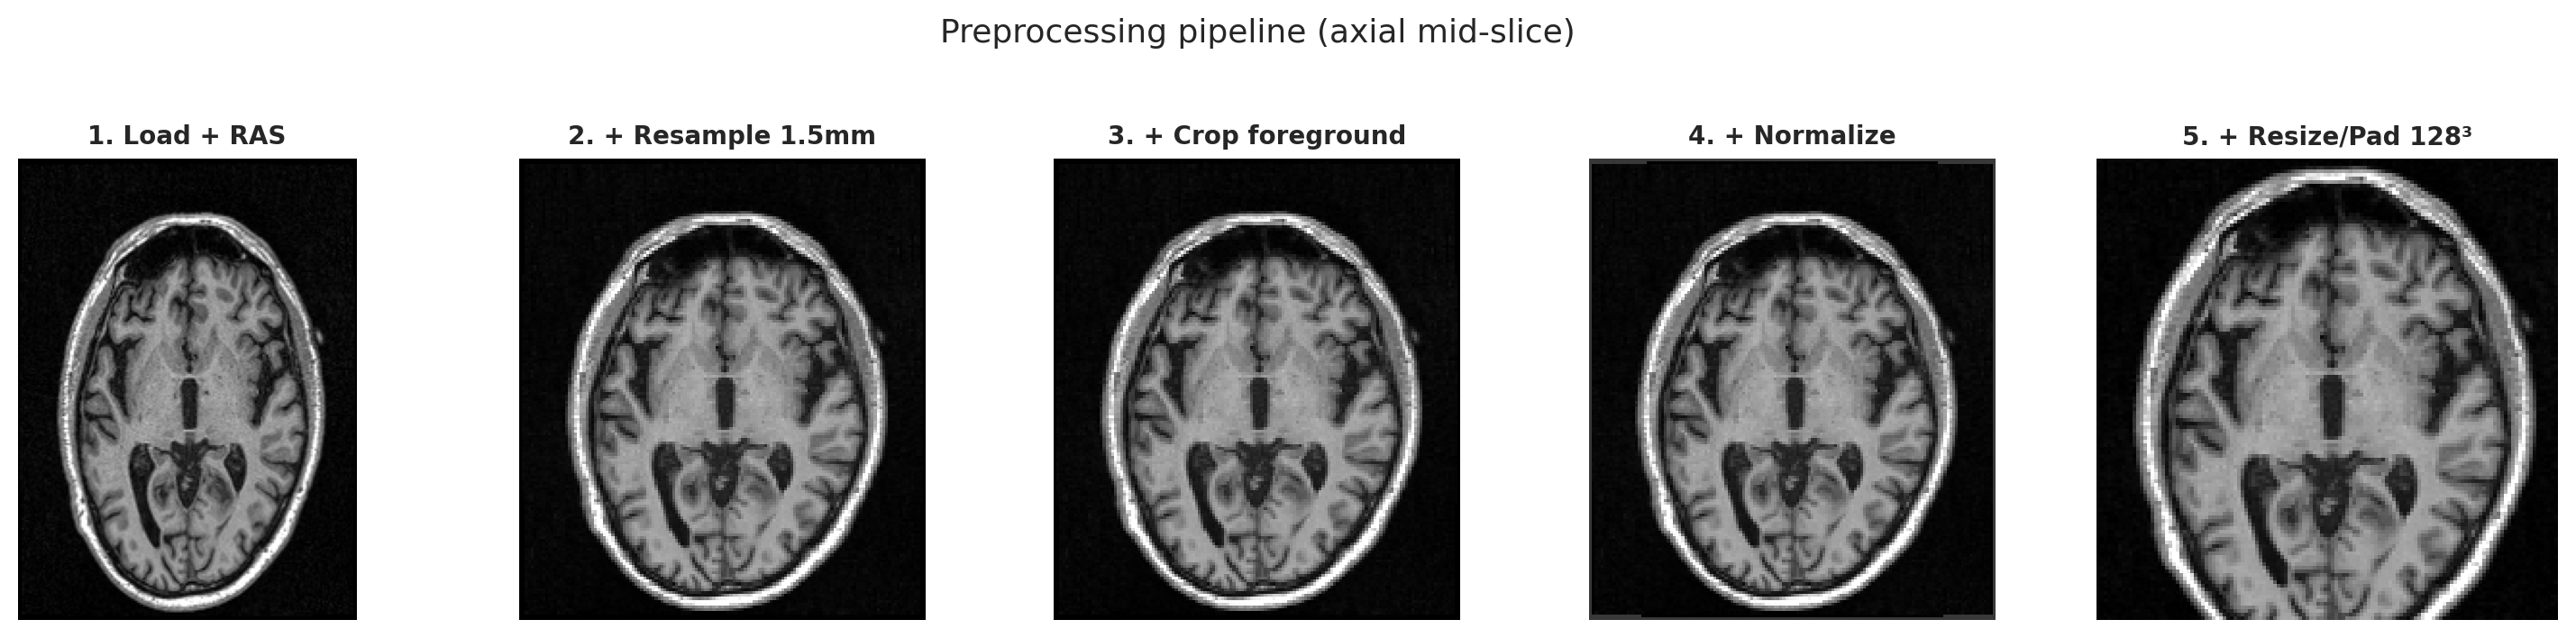
\includegraphics[width=15cm]{Images/ds_preprocessing.png}
    \caption[Preprocessing pipeline]{\textbf{Preprocessing pipeline.} Deterministic steps applied to every volume: reorientation, resampling, foreground crop, z-score normalization, and resizing.}
    \label{fig:preproc}
\end{figure}

\begin{figure}[H]
    \centering
    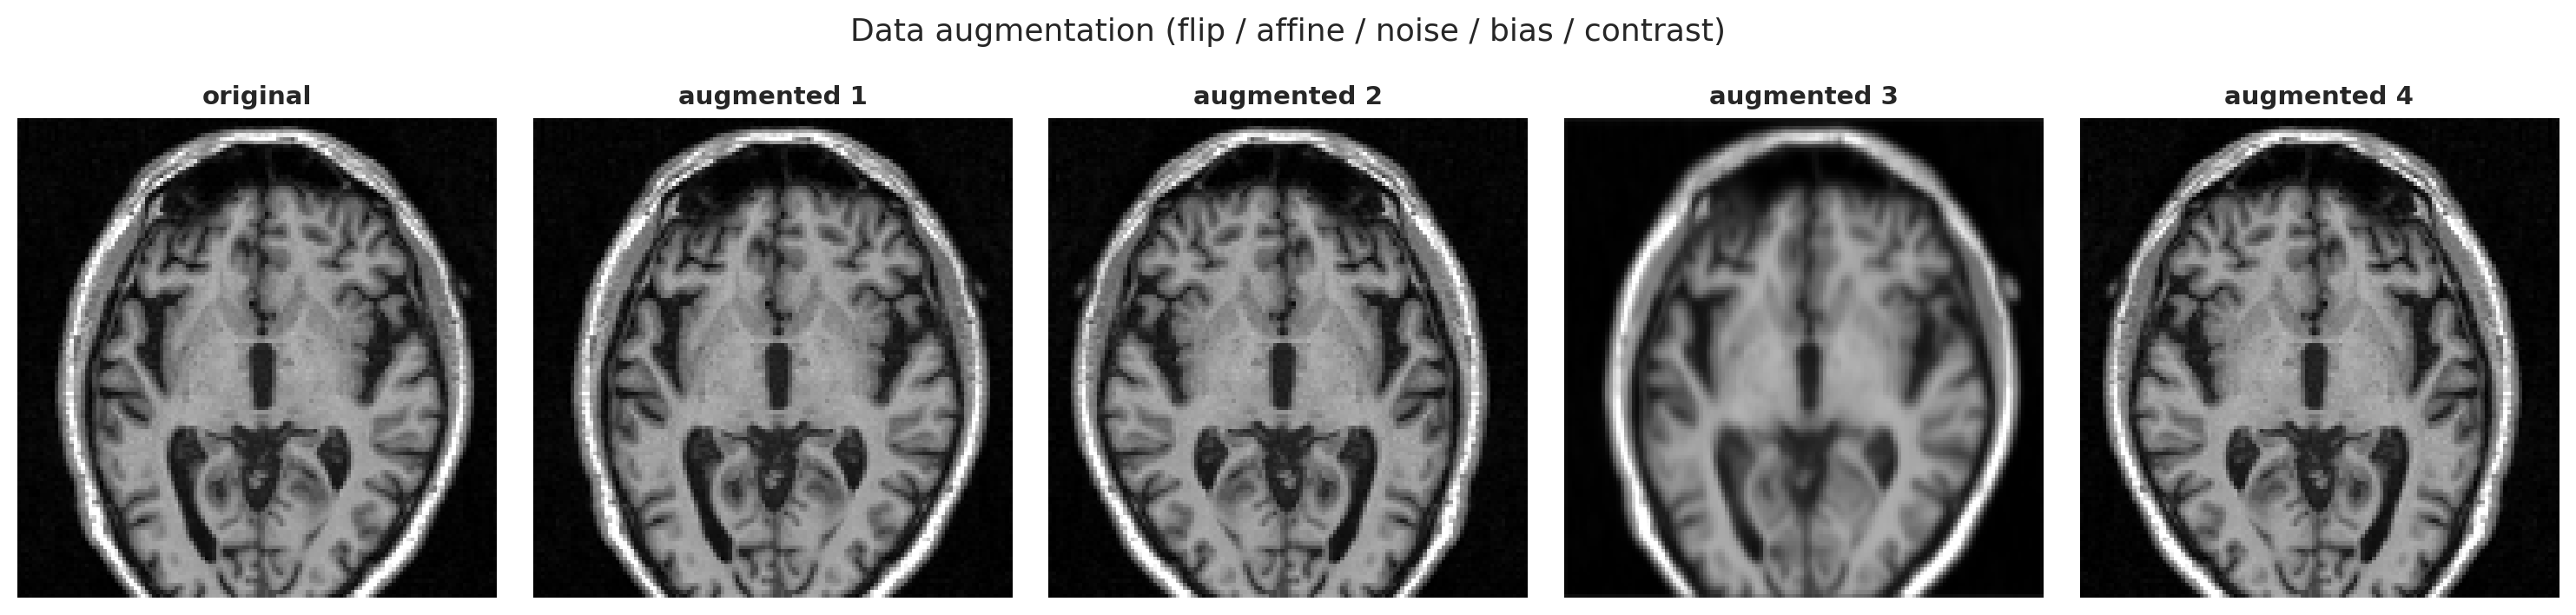
\includegraphics[width=14cm]{Images/ds_augmentation.png}
    \caption[Training augmentations]{\textbf{Training augmentations.} Examples of the training-only 3D augmentations (flips, affine, noise, intensity perturbations).}
    \label{fig:augment}
\end{figure}

\section{Model Development / Algorithm Design}
Five 3D backbones (and two hybrid combinations of them) are implemented behind a \emph{common interface}: every backbone exposes \texttt{forward\_features(x)} returning a $(B, \text{feat\_dim})$ vector, and a shared dropout + linear classifier head maps it to the class logits. Because the head and the training recipe are identical, the single-vs-hybrid comparison is genuinely apples-to-apples.

\subsection{Standalone Backbones}
\textbf{(1) 3D CNN --- DenseNet-121}~\cite{huang2017densely} (MONAI, trained from scratch). Densely connected 3D convolutions extract hierarchical local features (cortical thinning, ventricular enlargement, hippocampal atrophy); global-average pooling yields a 1024-D feature vector. This is the primary CNN baseline.\\
\textbf{(2) 3D ResNet --- MedicalNet pretrained.} A 3D ResNet~\cite{he2016deep} initialized with Tencent MedicalNet weights~\cite{chen2019med3d} (pretrained on 23 medical datasets) to test whether medical transfer learning helps on this cohort. It produces a 512-D feature vector.\\
\textbf{(3) 3D Vision Transformer (ViT)}~\cite{dosovitskiy2021image}. A compact ViT (hidden size 384, 6 layers, 6 heads, $16^3$ patch embedding on a $96^3$ input), trained from scratch, with token-average pooling. It tests how a pure global-attention model behaves on a small 3D dataset.\\
\textbf{(4) Swin Transformer}~\cite{liu2021swin,hatamizadeh2021swinunetr}. The hierarchical SwinUNETR-style encoder (shifted-window attention, embedding dim 48, four stages), with global-average pooling of the deepest stage. It is a strong, data-efficient transformer option for 3D medical imaging.

\subsection{Hybrid 3D CNN--ViT (Proposed)}
The proposed model runs two backbones in parallel on the same volume and fuses their features:
\begin{itemize}
    \item the \textbf{3D CNN branch} contributes local, texture-level anatomical detail;
    \item the \textbf{3D ViT branch} contributes global, long-range structural context.
\end{itemize}
Two fusion strategies are supported: \textbf{late concatenation} (the two feature vectors are concatenated and passed to the head) and \textbf{cross-attention} (the CNN feature attends to the transformer feature via a multi-head attention block). The fused representation goes through the shared dropout + linear head and a softmax. This design directly operationalizes the research question of whether combining local and global 3D features beats either alone. Algorithm~\ref{alg:hybrid} sketches the forward pass. Only late-concatenation fusion was trained and evaluated in this thesis; cross-attention is implemented but left to future work.

As a control for the role of the CNN branch, a second hybrid, \textbf{Swin--ViT}, fuses the Swin encoder (in place of DenseNet) with the same ViT branch by late concatenation. It contains no convolutional branch, so comparing it with CNN--ViT indicates how much of the hybrid's signal comes from the CNN. Because it differs from CNN--ViT in its first branch rather than in the fusion mechanism, it is a comparison of \emph{branch choice}, not of fusion strategy.

\begin{algorithm}[H]
\caption{Hybrid 3D CNN--ViT classification (late-concat fusion)}
\label{alg:hybrid}
\begin{algorithmic}[1]
\Require Preprocessed MRI volume $V \in \mathbb{R}^{1\times96\times96\times96}$
\Ensure Class prediction $\hat{y}$ and 3D importance map $H$
\State $f_{\text{cnn}} \gets \textsc{DenseNet3D.forwardFeatures}(V)$ \Comment{local features, 1024-D}
\State $f_{\text{vit}} \gets \textsc{ViT3D.forwardFeatures}(V)$ \Comment{global features, 384-D}
\State $z \gets \textsc{Concat}(f_{\text{cnn}}, f_{\text{vit}})$
\State $\text{logits} \gets \textsc{Linear}(\textsc{Dropout}(z))$
\State $\hat{y} \gets \textsc{Softmax}(\text{logits})$
\State $H \gets \textsc{GradCAM3D}(f_{\text{cnn}})$ \Comment{explainability overlay}
\State \Return $\hat{y}, H$
\end{algorithmic}
\end{algorithm}

\section{Training Recipe}
Within each task, all models share one recipe so that differences reflect the architecture, not the tuning (the binary and three-class recipes differ in loss, epochs, warmup, patience, and weight decay; the exact values per run are listed in Appendix~\ref{app:repro}):
\begin{itemize}
    \item \textbf{Optimizer:} AdamW~\cite{loshchilov2019decoupled}, learning rate $1\times10^{-4}$, weight decay $0.01$--$0.03$.
    \item \textbf{Schedule:} cosine decay~\cite{loshchilov2017sgdr} with linear warmup (5--8 epochs), up to 80--100 epochs.
    \item \textbf{Loss:} focal loss~\cite{lin2017focal} ($\gamma=2$) for the three-class task (to handle the MCI minority); class-weighted cross-entropy with label smoothing~\cite{muller2019does} $0.1$ for the binary task. Class weights / weighted sampling address imbalance. \authortodo{state exactly which imbalance corrections were active in each run --- class-weighted loss, weighted sampler, focal loss, or a combination. Stacking several corrections can over-correct towards the minority classes, which is relevant to the three-class ViT result in Chapter~\ref{cha:results}.}
    \item \textbf{Memory:} automatic mixed precision (AMP) + gradient accumulation (batch size 2, accumulation 4 $\rightarrow$ effective batch 8) + gradient clipping at 1.0, to fit 3D volumes in 16\,GB.
    \item \textbf{Regularization:} dropout (0.2), weight decay, heavy 3D augmentation, and early stopping on validation subject-level macro-F1 (patience 15--18).
    \item \textbf{Reproducibility:} every run seeds all RNGs, logs library versions, and saves its exact YAML config, the split file, per-fold metrics, and checkpoints.
\end{itemize}

\section{System Implementation / Modules Description}
The system is modular. The \textbf{Data module} indexes ADNI volumes by image-ID, builds subject-level loaders and the weighted sampler, and applies the MONAI transforms. The \textbf{Model module} contains the five backbones, the shared classifier head, and the hybrid fusion blocks behind the common \texttt{build\_model(cfg)} factory. The \textbf{Training module} runs AMP training, tracks validation subject-level macro-F1, early-stops, and checkpoints. The \textbf{Evaluation module} computes scan- and subject-level metrics, confusion matrices, and ROC curves, and aggregates folds into mean $\pm$ std summaries. The \textbf{Explainability module} generates Grad-CAM/Grad-CAM++/Integrated-Gradients/attention-rollout overlays for a chosen model and subject.

\section{Hardware and Software Requirements}
\textbf{Hardware.} Training was performed on a single NVIDIA RTX 5060 Ti (16\,GB), 32\,GB RAM. The 16\,GB budget dictates $96^3$--$128^3$ inputs, batch size 2 with gradient accumulation, and AMP. Inference (including explainability) runs comfortably on the same GPU.\\
\textbf{Software.} Python 3.10, PyTorch 2.11 (CUDA 12.8), MONAI 1.6, NiBabel 5.4, scikit-learn 1.4, NumPy 1.26, under Windows with an NVIDIA CUDA 12.x driver. All frameworks are open-source.

\section{Summary}
This chapter described the complete, reproducible methodology: a curated single-cohort (multi-site) ADNI dataset (1{,}132 scans / 395 subjects) evaluated under a strict subject-level five-fold protocol; a deterministic MONAI preprocessing pipeline; five 3D architectures sharing one interface, head, and training recipe; and a hybrid 3D CNN--ViT as the proposed model. The design prioritizes a fair, leakage-free comparison over headline accuracy, setting up the experimental results reported in Chapter~\ref{cha:results}.


\chapter{Experimental Results and Analysis} \label{cha:results}
This chapter reports the experimental results of the five 3D architectures on the ADNI cohort, under the strict subject-level five-fold protocol defined in Chapter~\ref{cha:MethodologyAndImplementationU}. Results are presented for the headline binary CN-vs-AD task and the harder three-class CN/MCI/AD benchmark, followed by an analysis of the single-vs-hybrid question, the effect of medical transfer learning, the behaviour of the transformer models, and an explainability study. All numbers are mean $\pm$ standard deviation across the five subject-disjoint folds (population standard deviation, $\mathrm{ddof}=0$), with macro-F1 as the primary metric. Every result should be read against the majority-class baseline of always predicting CN ($65.4\%$ binary, $52.2\%$ three-class accuracy), which is included in the main tables.

\section{Experimental Setup Recap}
Every model was trained and evaluated on the \emph{same} folds (\texttt{seed = 42}), with the same preprocessing, classifier head, imbalance handling, and evaluation; the backbone and its schedule differ (Appendix~\ref{app:repro}). Predictions are aggregated to the subject level by averaging a subject's per-scan softmax probabilities. Because CN is the majority class and MCI the minority, accuracy alone is misleading, so macro-F1 (the unweighted mean of per-class F1) is treated as the headline number and drives model selection and early stopping.

\section{Binary CN-vs-AD Results (Headline)}
Table~\ref{tab:binary} reports the binary task. The proposed \textbf{hybrid 3D CNN--ViT} has the highest mean at $82.2\%$ accuracy and $0.802$ macro-F1, but the from-scratch 3D DenseNet CNN ($81.0\%$, $0.788$) is statistically indistinguishable from it (Section~\ref{sec:rq1}). Both clear the $65.4\%$ majority-class baseline by a wide margin. The Swin+ViT hybrid and the MedicalNet-pretrained ResNet trail by roughly 12 points, sit only about 4--5 points above the majority baseline in accuracy, and show markedly higher variance across folds. Standalone ViT and Swin models were not run on the binary task.

\begin{table}[H]
\centering
\caption{Binary CN-vs-AD, subject-level 5-fold cross-validation (mean $\pm$ std).}
\label{tab:binary}
\begin{tabular}{|l|c|c|c|}
\hline
\textbf{Model} & \textbf{Accuracy} & \textbf{Macro-F1} & \textbf{Weighted-F1} \\
\hline
\textbf{Hybrid 3D CNN--ViT (concat)} & \textbf{0.822 $\pm$ 0.057} & \textbf{0.802 $\pm$ 0.062} & \textbf{0.820} \\
3D CNN (DenseNet-121, scratch) & 0.810 $\pm$ 0.041 & 0.788 $\pm$ 0.062 & 0.807 \\
Hybrid Swin--ViT & 0.702 $\pm$ 0.070 & 0.662 $\pm$ 0.101 & 0.696 \\
3D ResNet (MedicalNet pretrained) & 0.698 $\pm$ 0.139 & 0.654 $\pm$ 0.168 & 0.678 \\
\hline
\textit{Majority-class baseline (always CN)} & \textit{0.654} & \textit{0.395} & \textit{0.517} \\
\hline
\end{tabular}
\end{table}

\begin{figure}[H]
    \centering
    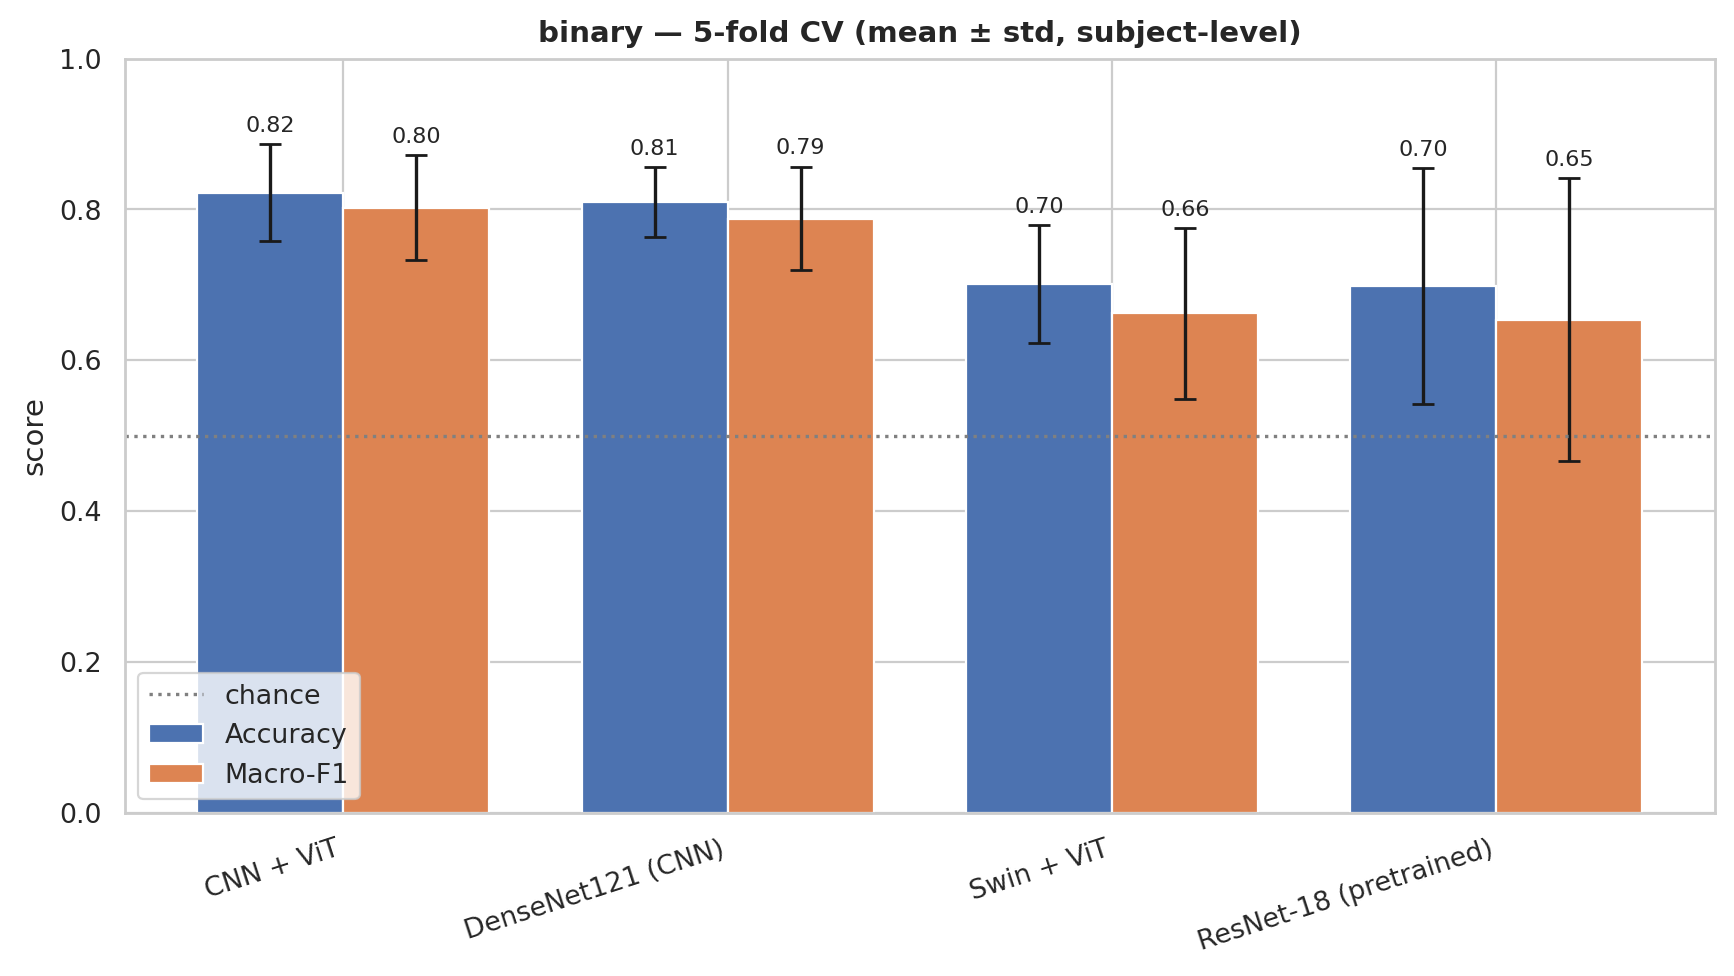
\includegraphics[width=14cm]{Images/res_bar_binary.png}
    \caption[Binary model comparison]{\textbf{Binary model comparison.} Per-model accuracy, macro-F1, and weighted-F1 for CN-vs-AD (mean $\pm$ std over five folds).}
    \label{fig:bar_binary}
\end{figure}

Figure~\ref{fig:confusion_binary} shows the fold-summed, row-normalised confusion matrices of all four binary models. For CNN--ViT and DenseNet the errors are roughly balanced between the two directions (CN recall $0.83$--$0.86$, AD recall $0.75$--$0.77$), so neither model is simply defaulting to the majority class; Swin+ViT, by contrast, misses $43\%$ of AD subjects. Figure~\ref{fig:perf_binary} gives ROC, precision--recall, and calibration curves for the DenseNet CNN. \textbf{These diagnostics cover only three of the five folds (189 subjects)} because checkpoints for the remaining folds were not retained; on that subset the CNN reaches $78.3\%$ accuracy and a pooled ROC-AUC of $0.82$. The calibration curve shows that the model is over-confident in its highest-probability bins.

\begin{figure}[H]
    \centering
    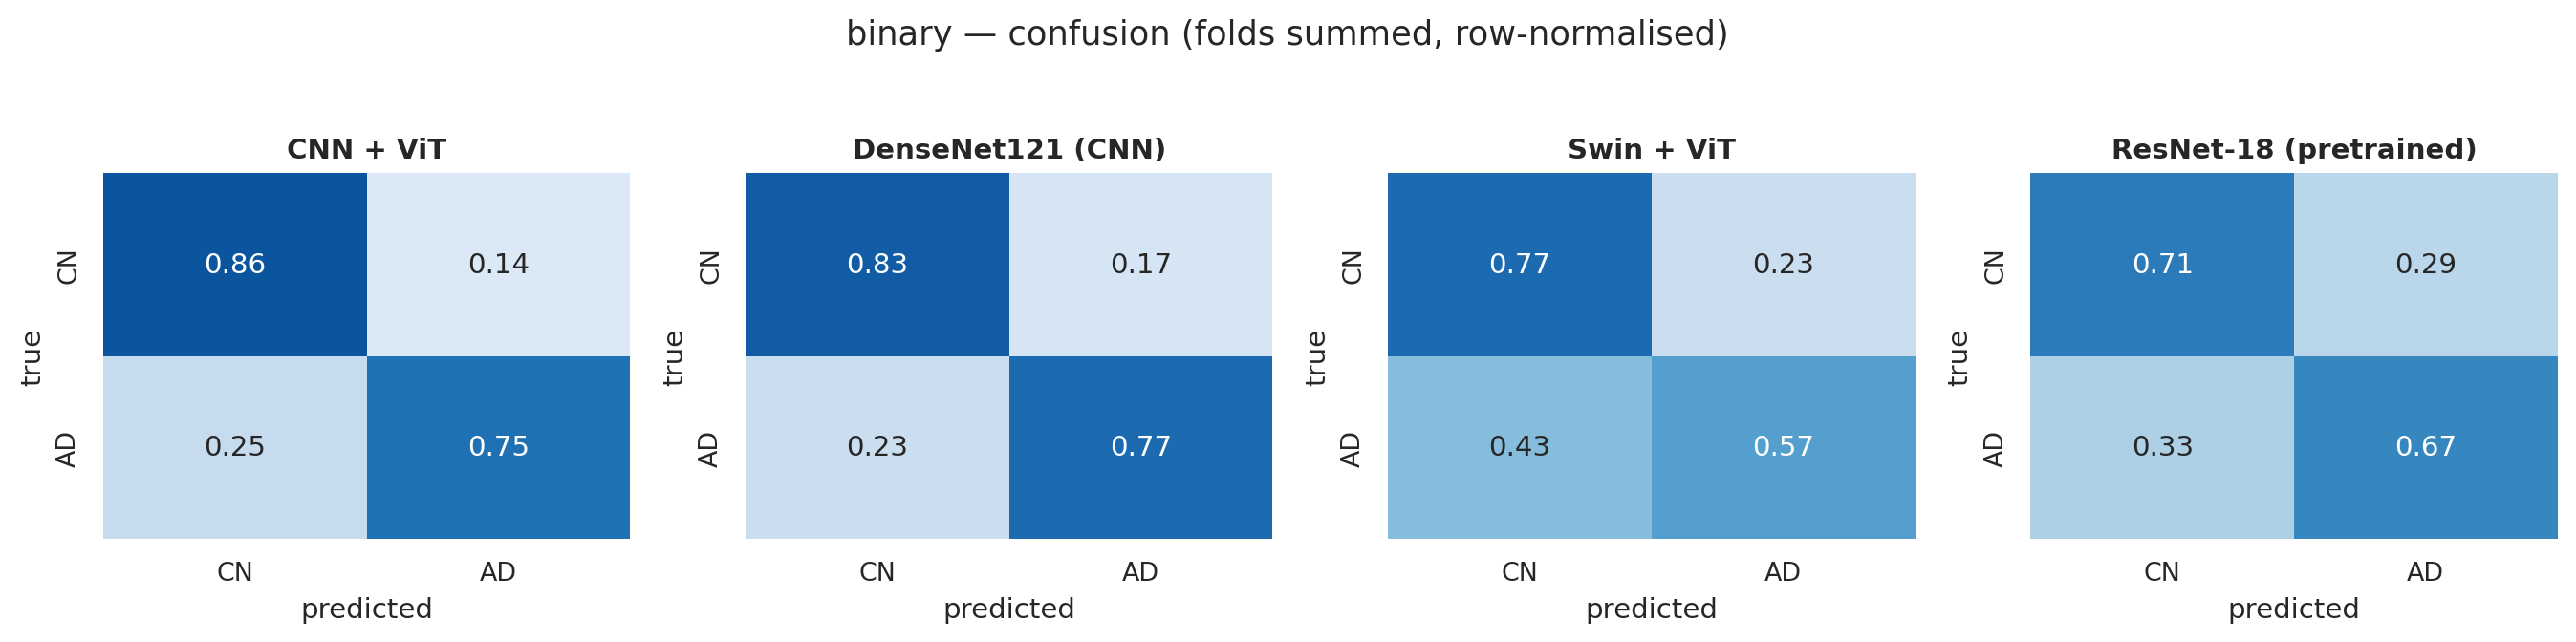
\includegraphics[width=10cm]{Images/res_confusion_binary.png}
    \caption[Binary confusion matrices]{\textbf{Binary confusion matrices.} Fold-summed, row-normalised CN-vs-AD confusion for all four binary models (subject-level predictions).}
    \label{fig:confusion_binary}
\end{figure}

\begin{figure}[H]
    \centering
    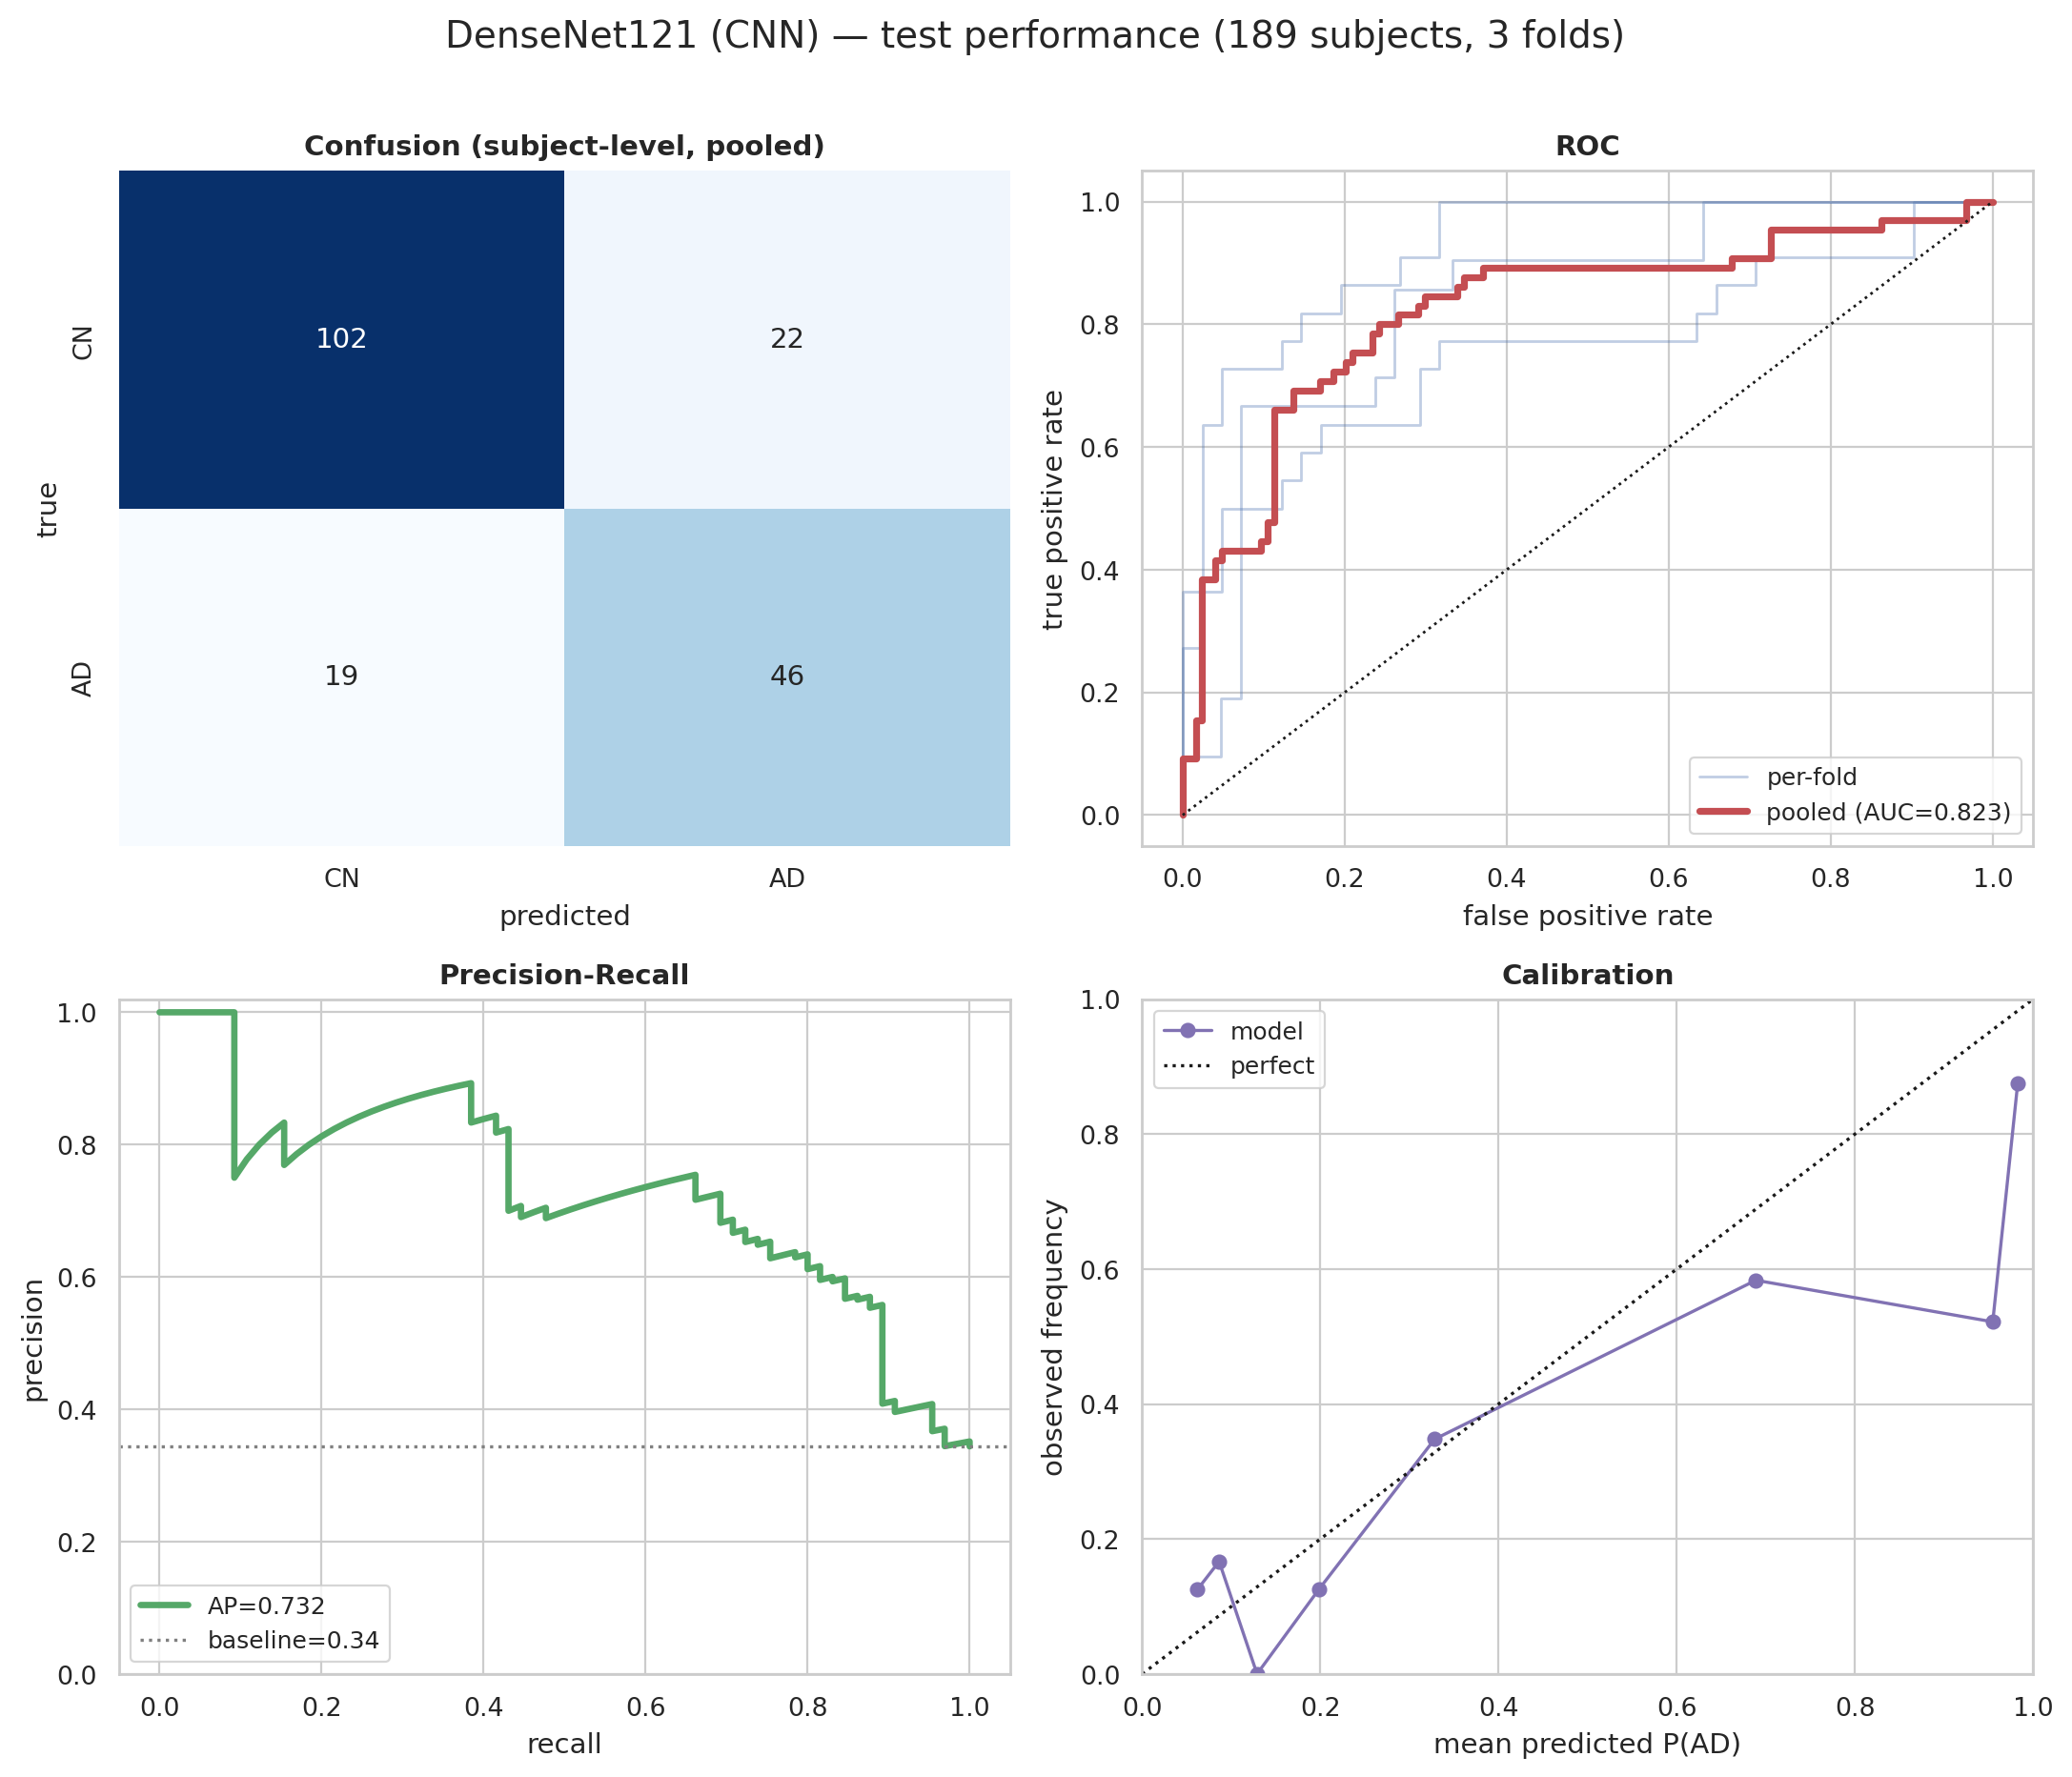
\includegraphics[width=15cm]{Images/res_perf_binary_cnn.png}
    \caption[Binary diagnostics (3 of 5 folds)]{\textbf{Binary diagnostics (3 of 5 folds, 189 subjects).} Confusion, per-fold and pooled ROC, precision--recall, and calibration for the 3D CNN (CN-vs-AD), computed on the three folds whose checkpoints were retained.}
    \label{fig:perf_binary}
\end{figure}

\section{Three-Class CN/MCI/AD Results (Honest Benchmark)}
Adding MCI --- the transitional stage whose MRI signature overlaps both neighbours --- sharply lowers performance for every model (Table~\ref{tab:3class}). The Swin Transformer and the 3D CNN are tied at the top ($\sim\!57\%$ accuracy, $\sim\!0.53$ macro-F1; paired fold-wise test $t=0.70$, $p\approx0.5$), only about five points above the $52.2\%$ accuracy of always predicting CN --- although their macro-F1 is more than twice the baseline's $0.23$, showing that they do separate the classes to some degree. The from-scratch ViT falls \emph{below} the majority baseline (Section~\ref{sec:vit_collapse}). The proposed CNN--ViT hybrid was not trained on the three-class task.

\begin{table}[H]
\centering
\caption{Three-class CN/MCI/AD, subject-level 5-fold cross-validation (mean $\pm$ std).}
\label{tab:3class}
\begin{tabular}{|l|c|c|c|}
\hline
\textbf{Model} & \textbf{Accuracy} & \textbf{Macro-F1} & \textbf{Weighted-F1} \\
\hline
\textbf{Swin Transformer} & \textbf{0.577 $\pm$ 0.098} & \textbf{0.537 $\pm$ 0.078} & \textbf{0.573} \\
3D CNN (DenseNet-121, scratch) & 0.572 $\pm$ 0.092 & 0.524 $\pm$ 0.071 & 0.560 \\
3D ViT (from scratch) & 0.286 $\pm$ 0.015 & 0.256 $\pm$ 0.012 & 0.184 \\
\hline
\textit{Majority-class baseline (always CN)} & \textit{0.522} & \textit{0.229} & \textit{0.358} \\
\hline
\end{tabular}
\end{table}

\begin{figure}[H]
    \centering
    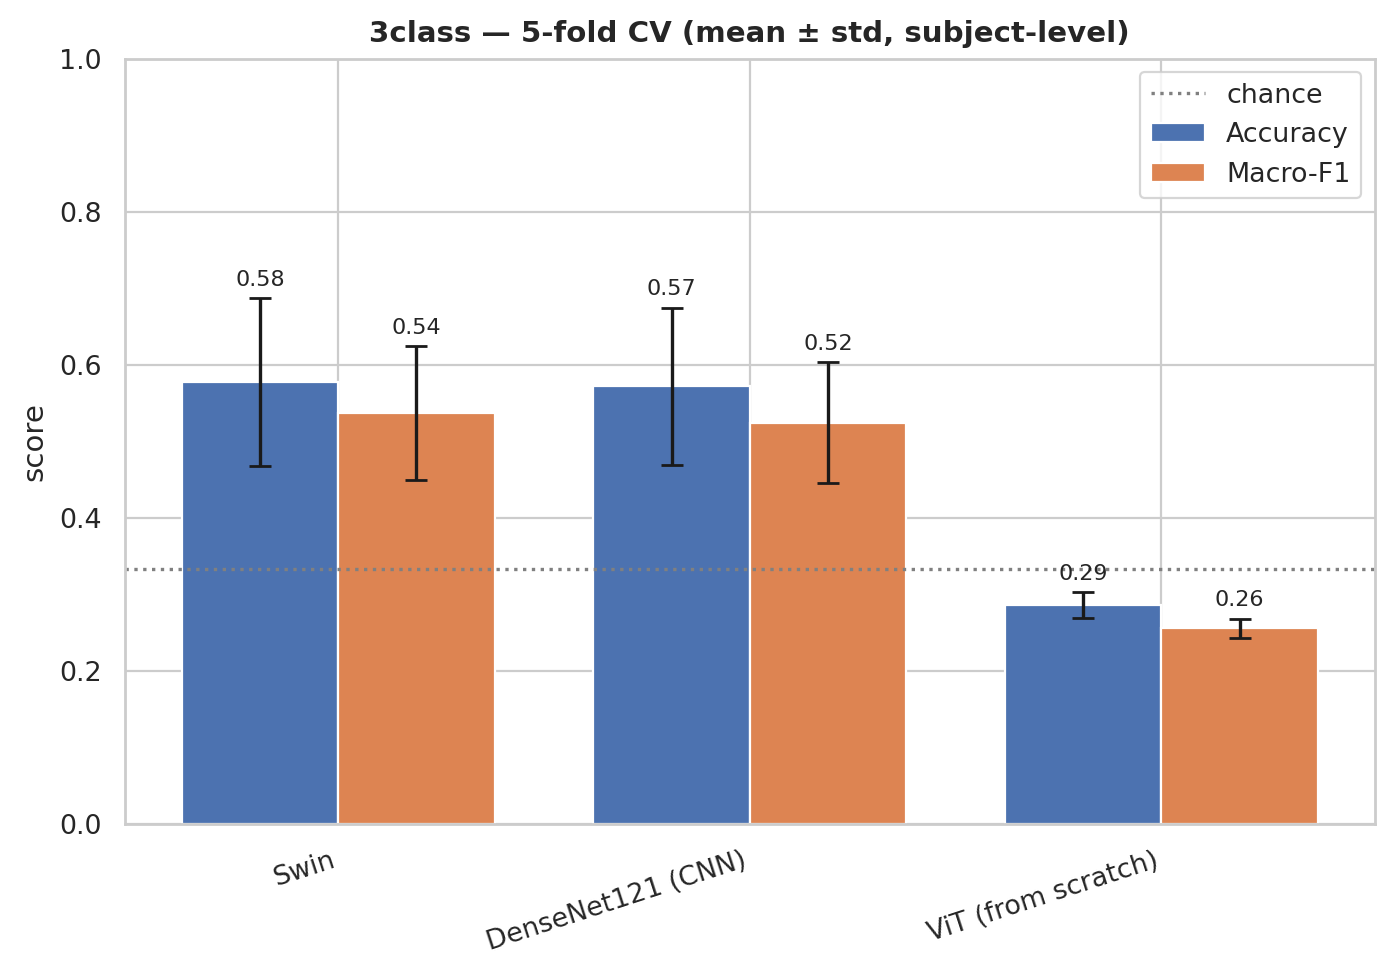
\includegraphics[width=14cm]{Images/res_bar_3class.png}
    \caption[Three-class model comparison]{\textbf{Three-class model comparison.} Per-model accuracy, macro-F1, and weighted-F1 for CN/MCI/AD (mean $\pm$ std over five folds).}
    \label{fig:bar_3class}
\end{figure}

The per-class breakdown is revealing: pooled over folds, CN reaches a per-class F1 of about $0.65$ and AD $0.55$--$0.61$, whereas \textbf{MCI reaches only $0.37$--$0.41$} (Table~\ref{tab:3class_perclass}). The confusion is overwhelmingly MCI being absorbed into CN or AD, exactly as expected for a stage that is clinically defined as intermediate. This is why a leakage-free three-class accuracy in the high-90s (as claimed by several slice-level studies in Chapter~\ref{cha:LiteratureReviewU}) is not credible on 395 subjects: the ceiling here is honest, and MCI is the bottleneck.

\section{Per-Fold Results and Fold Variance}
Because the cohort is small, a single split is unreliable; reporting every fold exposes how stable each model actually is. Tables~\ref{tab:binary_folds} and \ref{tab:3class_folds} give the per-fold macro-F1 for the binary and three-class tasks, and Figure~\ref{fig:box} shows the corresponding spread.

\begin{table}[H]
\centering
\caption{Binary CN-vs-AD per-fold macro-F1 (subject-level).}
\label{tab:binary_folds}
\begin{tabular}{|l|c|c|c|c|c|c|}
\hline
\textbf{Model} & \textbf{F1} & \textbf{F2} & \textbf{F3} & \textbf{F4} & \textbf{F5} & \textbf{Mean $\pm$ std} \\
\hline
Hybrid CNN--ViT & 0.716 & 0.857 & 0.743 & 0.821 & 0.873 & \textbf{0.802 $\pm$ 0.062} \\
CNN (DenseNet) & 0.768 & 0.810 & 0.678 & 0.834 & 0.850 & 0.788 $\pm$ 0.062 \\
Hybrid Swin--ViT & 0.672 & 0.723 & 0.700 & 0.750 & 0.466 & 0.662 $\pm$ 0.101 \\
ResNet (pretrained) & 0.775 & 0.449 & 0.449 & 0.779 & 0.816 & 0.654 $\pm$ 0.168 \\
\hline
\end{tabular}
\end{table}

The ResNet row is the clearest illustration of instability: three folds are strong ($\sim\!0.78$--$0.82$) while two collapse to $0.449$, halving the mean and inflating the standard deviation. This bimodal pattern --- rather than a uniformly weak model --- is consistent with the early-stopping hypothesis discussed below. By contrast, the CNN and the CNN--ViT hybrid stay above $0.67$ macro-F1 in every fold, although each still varies by about $0.15$--$0.17$ between its best and worst fold.

\begin{table}[H]
\centering
\caption{Three-class CN/MCI/AD per-fold macro-F1 (subject-level).}
\label{tab:3class_folds}
\begin{tabular}{|l|c|c|c|c|c|c|}
\hline
\textbf{Model} & \textbf{F1} & \textbf{F2} & \textbf{F3} & \textbf{F4} & \textbf{F5} & \textbf{Mean $\pm$ std} \\
\hline
Swin Transformer & 0.564 & 0.471 & 0.457 & 0.675 & 0.518 & \textbf{0.537 $\pm$ 0.078} \\
CNN (DenseNet) & 0.592 & 0.433 & 0.489 & 0.622 & 0.487 & 0.524 $\pm$ 0.071 \\
ViT (scratch) & 0.261 & 0.238 & 0.254 & 0.273 & 0.253 & 0.256 $\pm$ 0.012 \\
\hline
\end{tabular}
\end{table}

\begin{figure}[H]
    \centering
    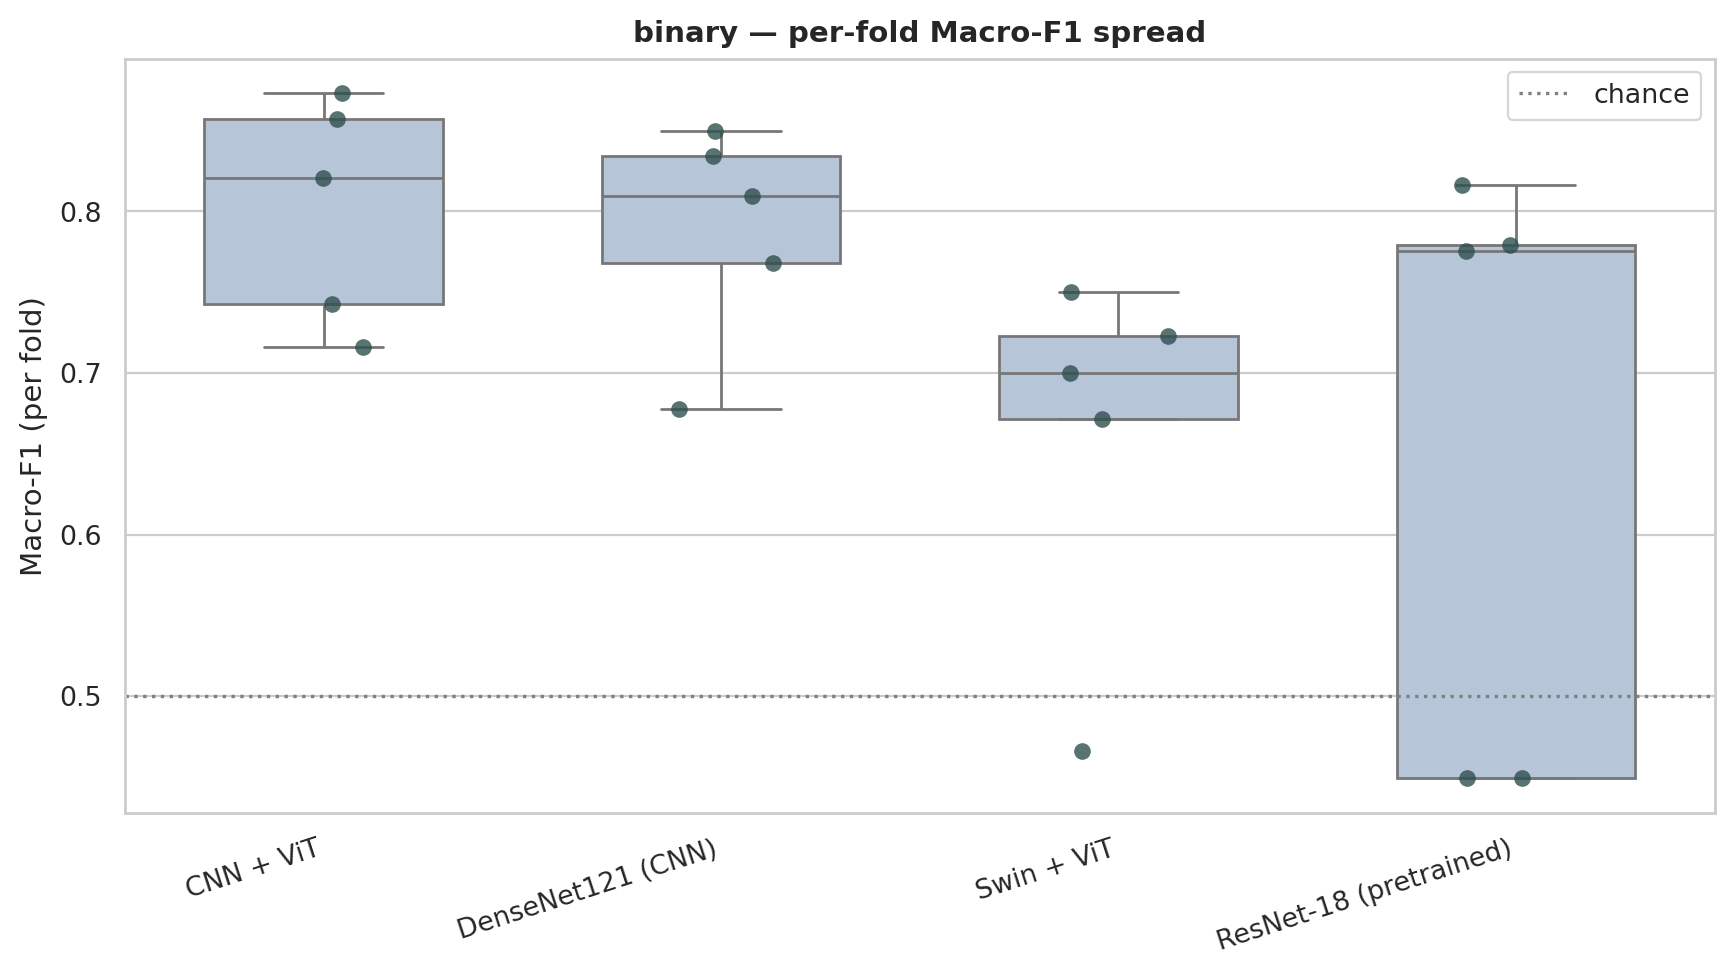
\includegraphics[width=7.6cm]{Images/res_box_binary.png}\hfill
    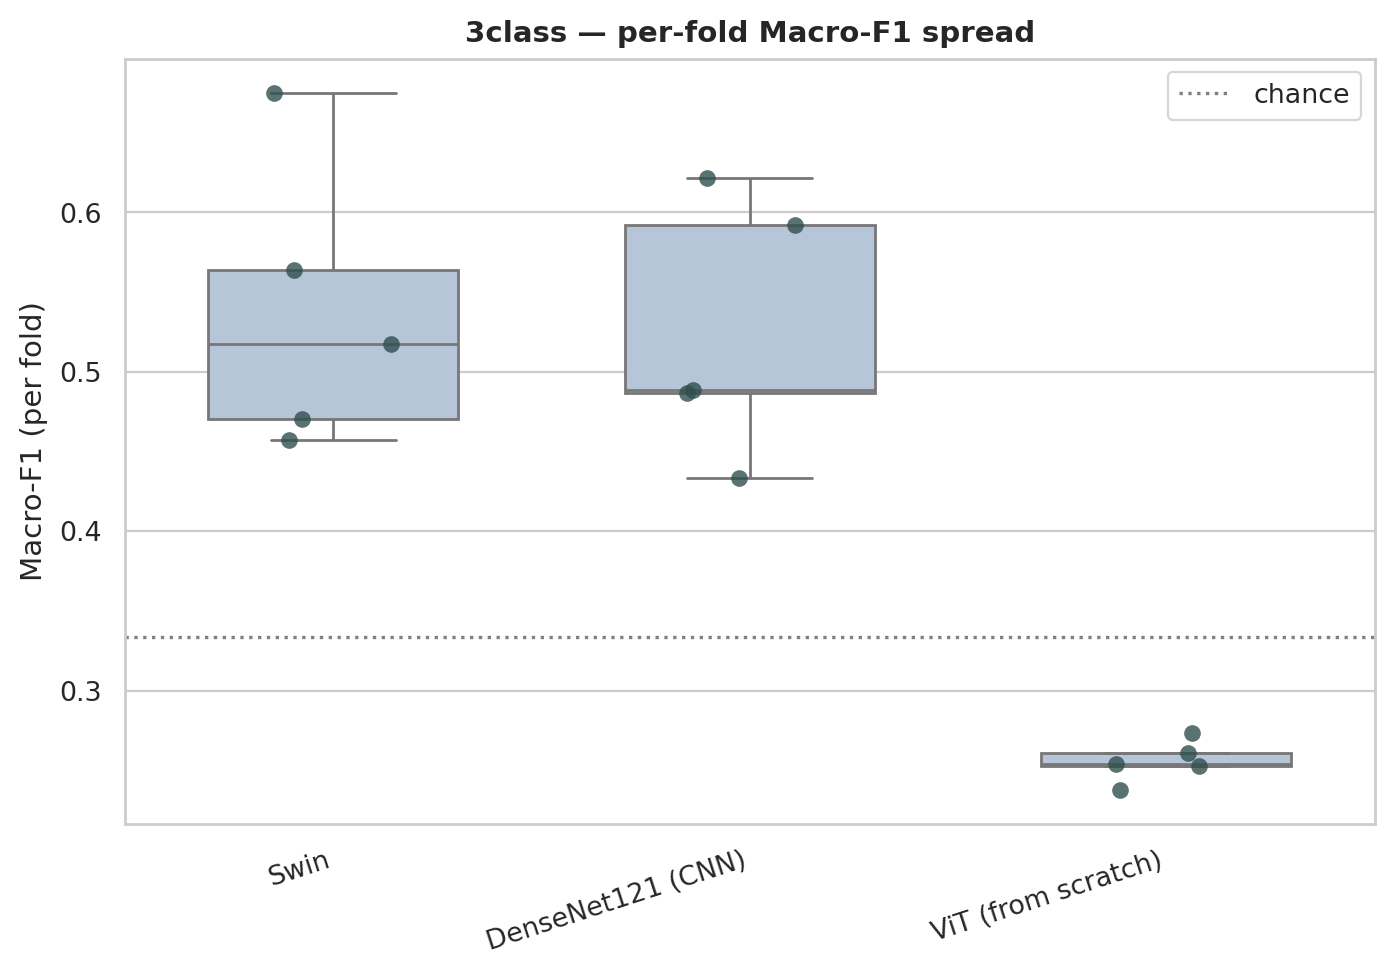
\includegraphics[width=7.6cm]{Images/res_box_3class.png}
    \caption[Fold variance]{\textbf{Fold variance.} Per-fold spread of macro-F1 for the binary (left) and three-class (right) tasks.}
    \label{fig:box}
\end{figure}

\section{Per-Class Performance}
Tables~\ref{tab:binary_perclass} and \ref{tab:3class_perclass} give the pooled per-class precision, recall, and F1 (aggregated over all five test folds). In the binary task both classes are recovered well, with the smaller AD class trailing the majority CN class by roughly $0.11$--$0.12$ F1 --- a modest, expected imbalance gap. In the three-class task the picture is dominated by MCI: its F1 ($0.37$--$0.41$) is only about half that of CN, and its low recall shows that a large fraction of true MCI subjects are pushed into the neighbouring CN or AD classes. This quantifies the qualitative claim that MCI is the bottleneck of the whole problem.

\begin{table}[H]
\centering
\caption{Binary CN-vs-AD pooled per-class metrics.}
\label{tab:binary_perclass}
\begin{tabular}{|l|l|c|c|c|c|}
\hline
\textbf{Model} & \textbf{Class} & \textbf{Precision} & \textbf{Recall} & \textbf{F1} & \textbf{Support} \\
\hline
\multirow{2}{*}{Hybrid CNN--ViT} & CN & 0.868 & 0.859 & 0.863 & 206 \\
                                 & AD & 0.739 & 0.752 & 0.745 & 109 \\
\hline
\multirow{2}{*}{CNN (DenseNet)}  & CN & 0.872 & 0.830 & 0.851 & 206 \\
                                 & AD & 0.706 & 0.771 & 0.737 & 109 \\
\hline
\end{tabular}
\end{table}

\begin{table}[H]
\centering
\caption{Three-class CN/MCI/AD pooled per-class metrics.}
\label{tab:3class_perclass}
\begin{tabular}{|l|l|c|c|c|c|}
\hline
\textbf{Model} & \textbf{Class} & \textbf{Precision} & \textbf{Recall} & \textbf{F1} & \textbf{Support} \\
\hline
\multirow{3}{*}{Swin} & CN  & 0.685 & 0.612 & 0.646 & 206 \\
                      & MCI & 0.366 & 0.375 & 0.370 & 80 \\
                      & AD  & 0.558 & 0.661 & 0.605 & 109 \\
\hline
\multirow{3}{*}{CNN}  & CN  & 0.653 & 0.641 & 0.647 & 206 \\
                      & MCI & 0.416 & 0.400 & 0.408 & 80 \\
                      & AD  & 0.534 & 0.569 & 0.551 & 109 \\
\hline
\end{tabular}
\end{table}

\section{Training Dynamics}
Figure~\ref{fig:tc} plots the training loss and validation subject-level macro-F1 across epochs for two representative binary runs. The from-scratch CNN's training loss falls steadily, while its validation macro-F1 rises to the $0.75$--$0.9$ range but fluctuates by up to $\pm0.1$ from epoch to epoch (only the folds whose logs were retained are plotted). The transformer-heavy runs are noisier and slower to rise, consistent with their weaker inductive bias. Figure~\ref{fig:tc_vit} shows the three-class ViT: its training loss barely decreases and its validation macro-F1 stays between about $0.1$ and $0.25$ throughout, a training-curve view of its collapse.

\begin{figure}[H]
    \centering
    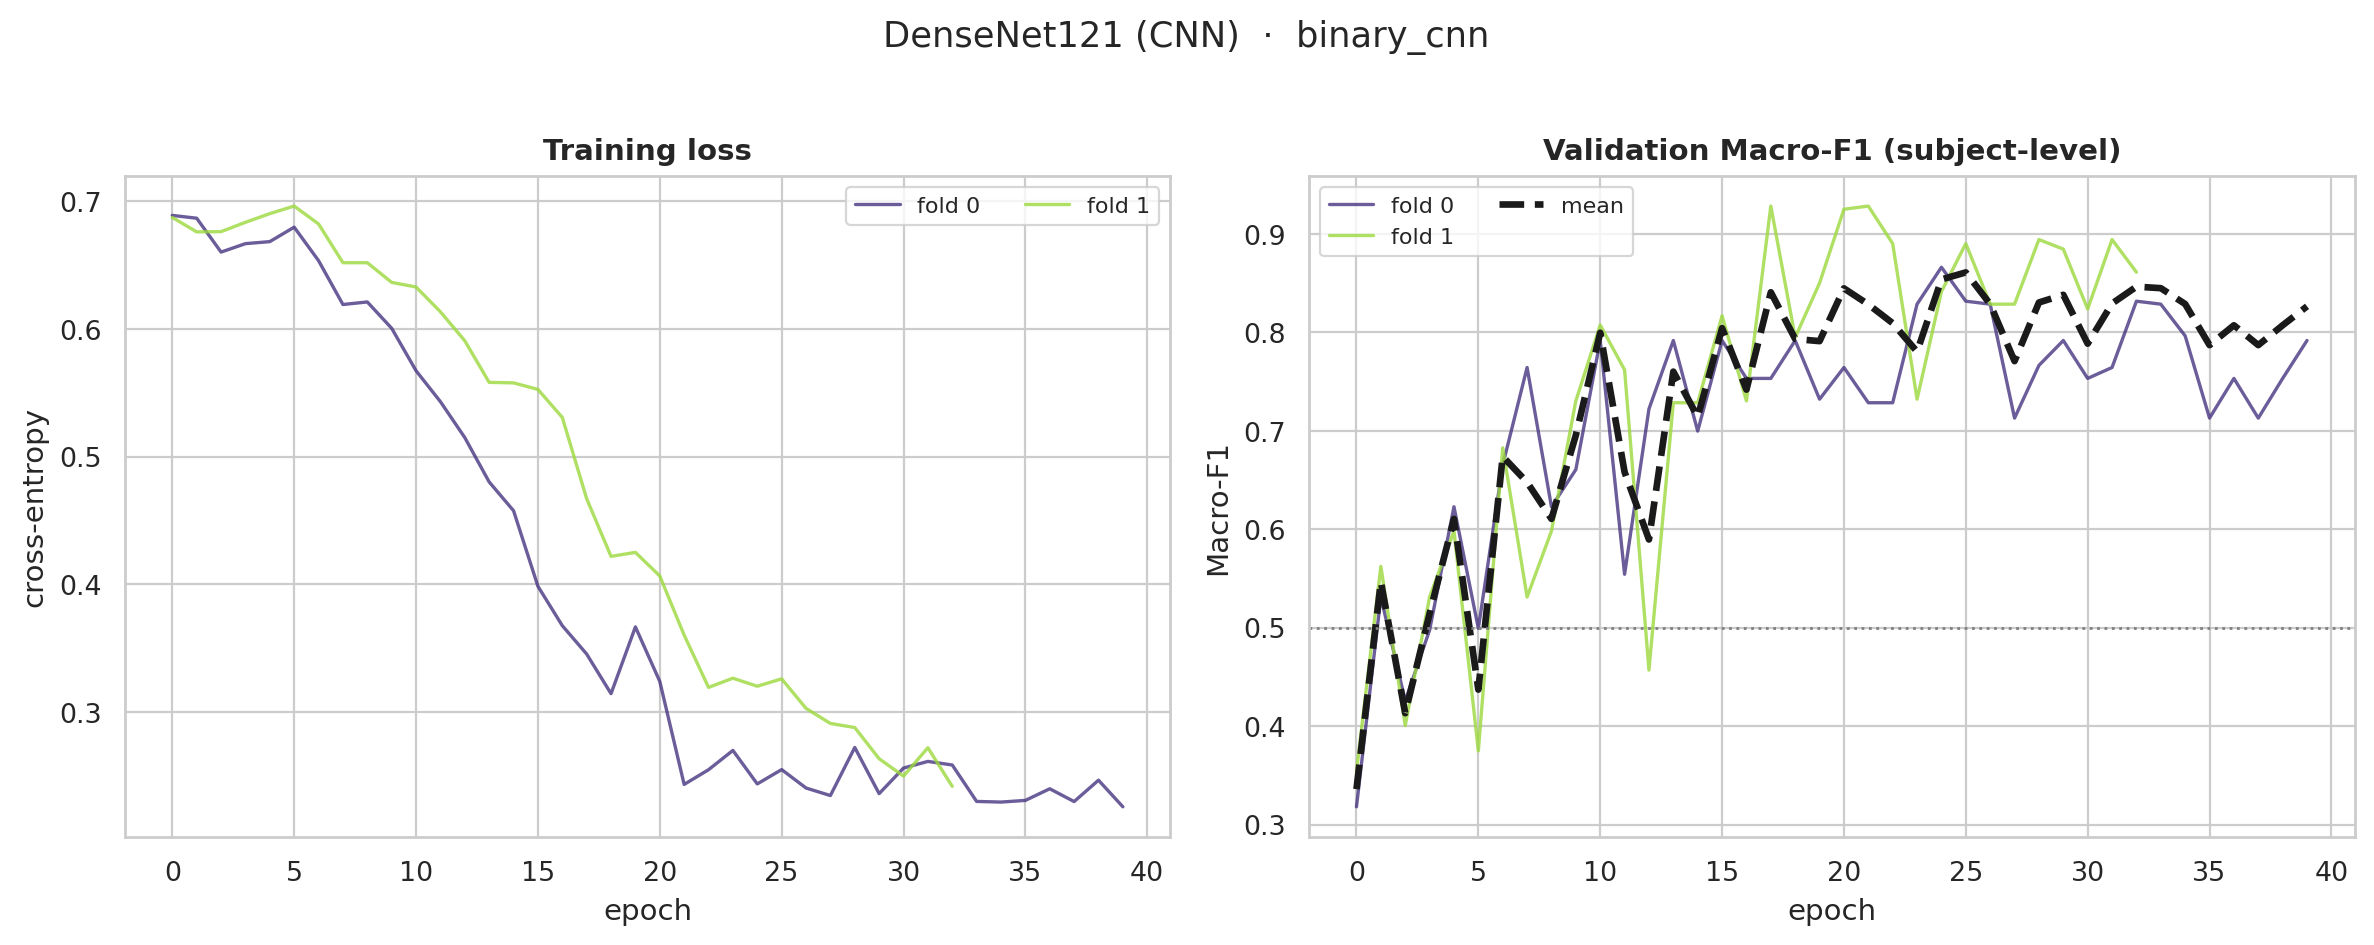
\includegraphics[width=7.6cm]{Images/tc_binary_cnn.png}\hfill
    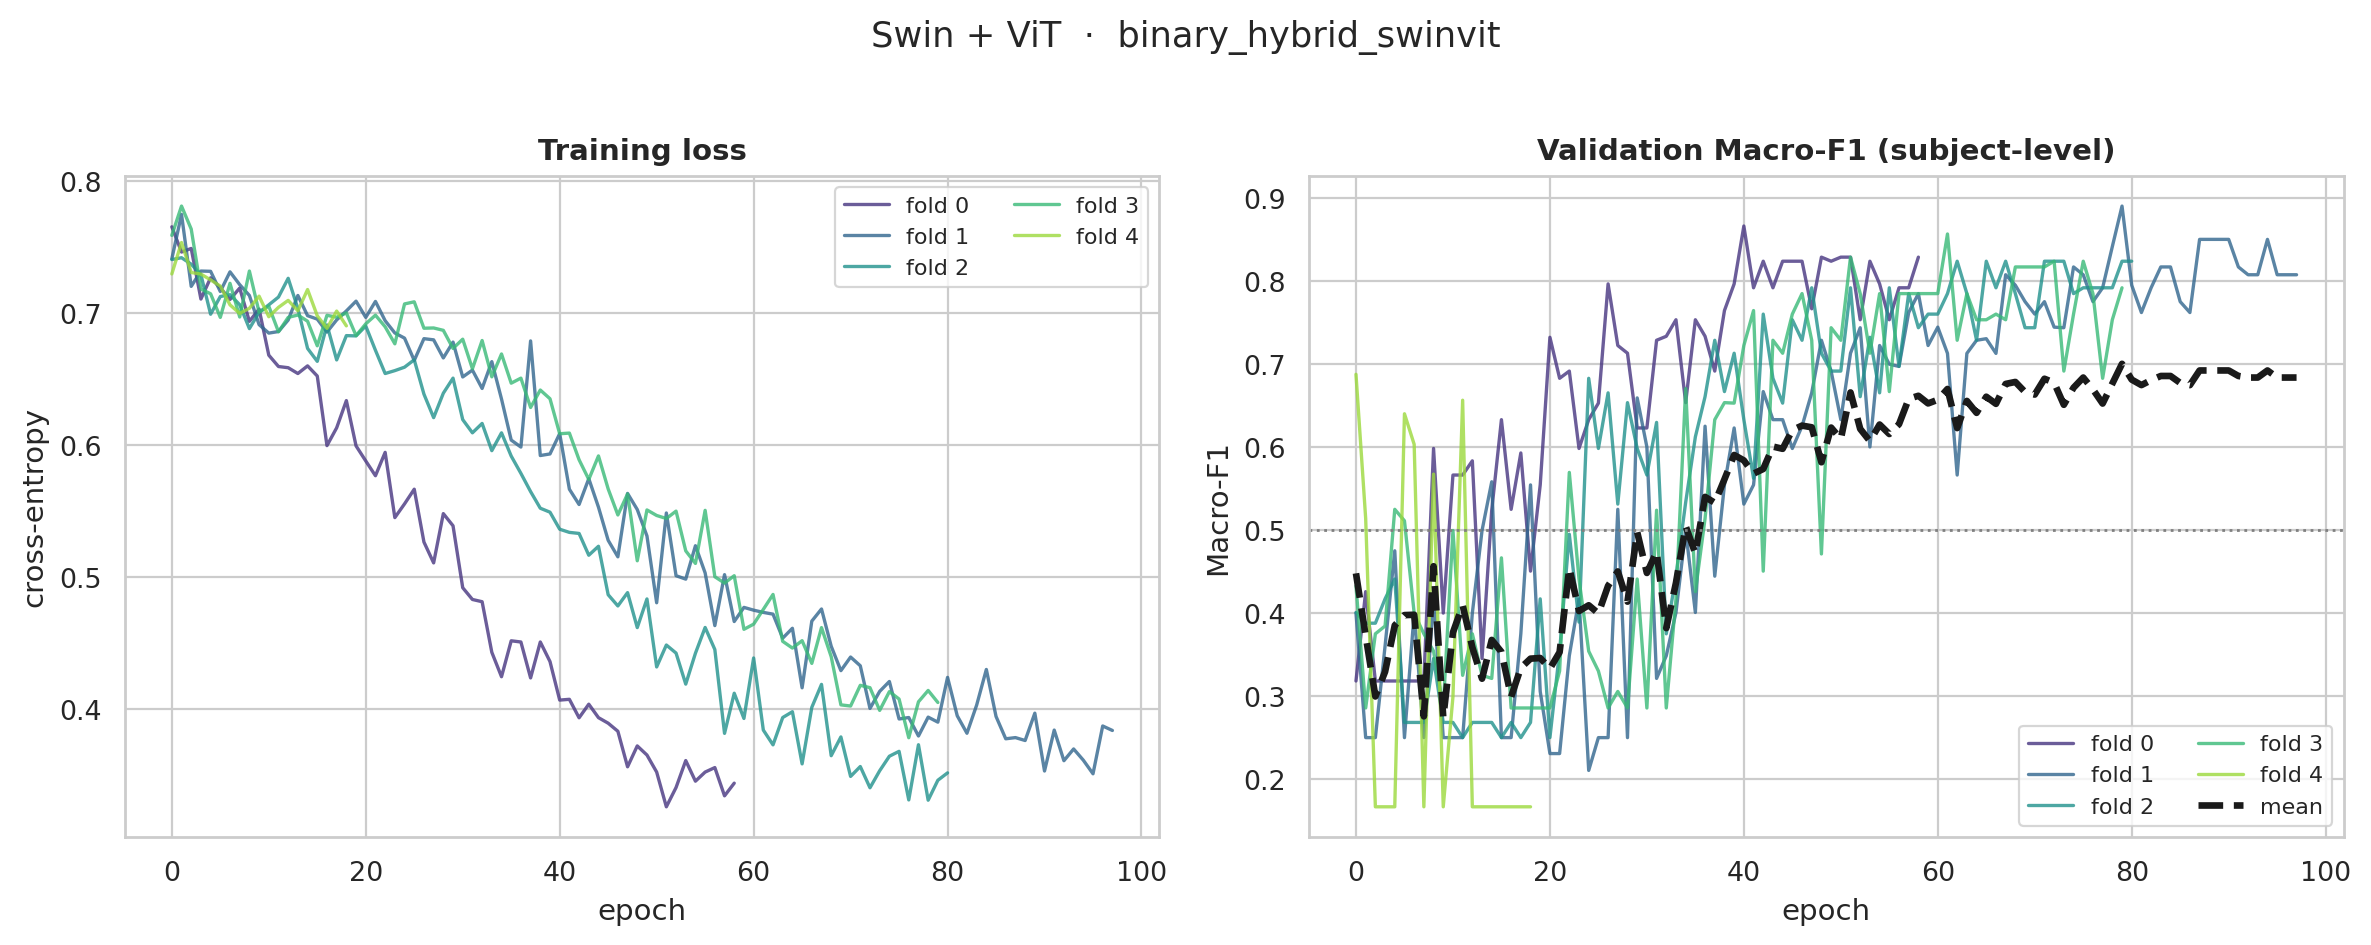
\includegraphics[width=7.6cm]{Images/tc_binary_hybrid_swinvit.png}
    \caption[Binary training curves]{\textbf{Binary training curves.} Per-fold training loss and validation macro-F1: binary CNN (left) and binary Swin--ViT hybrid (right).}
    \label{fig:tc}
\end{figure}

\begin{figure}[H]
    \centering
    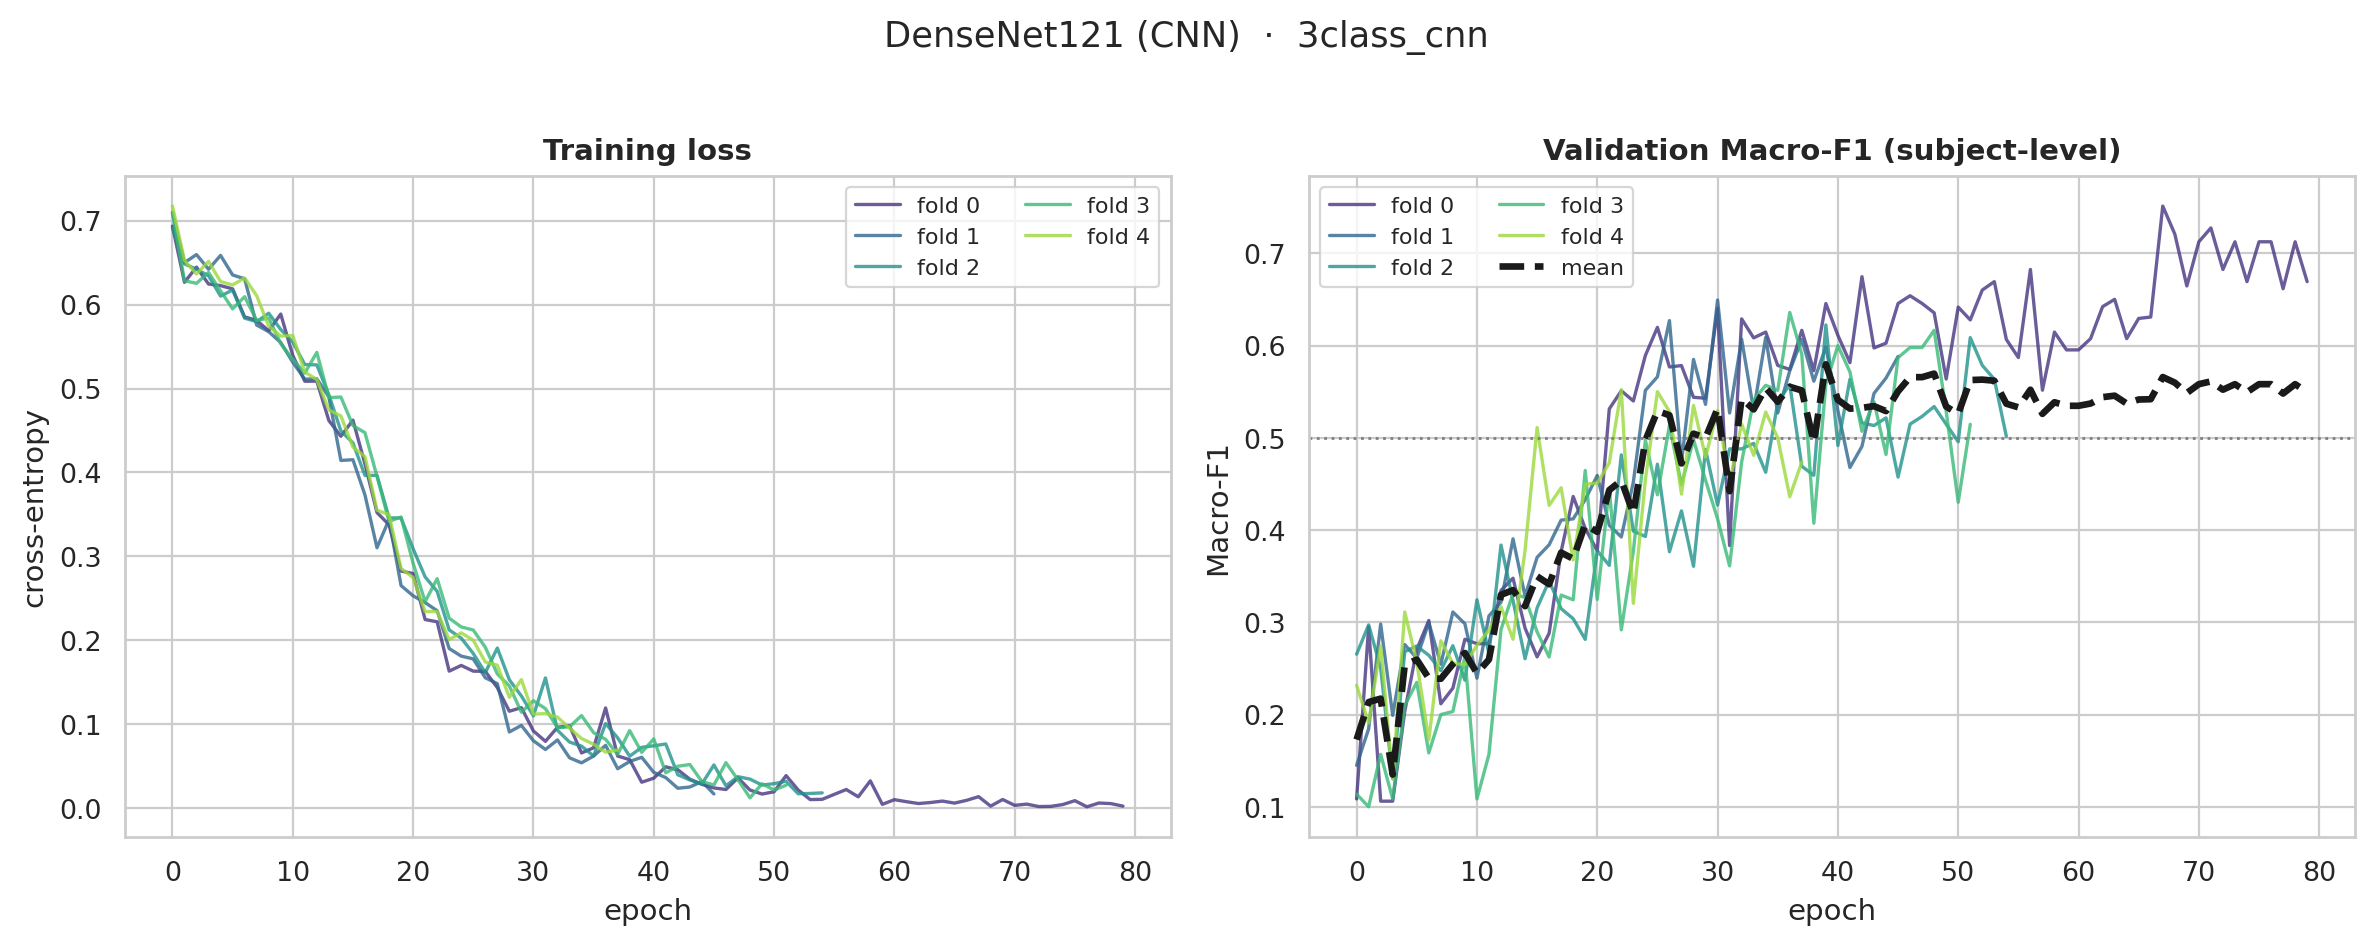
\includegraphics[width=7.6cm]{Images/tc_3class_cnn.png}\hfill
    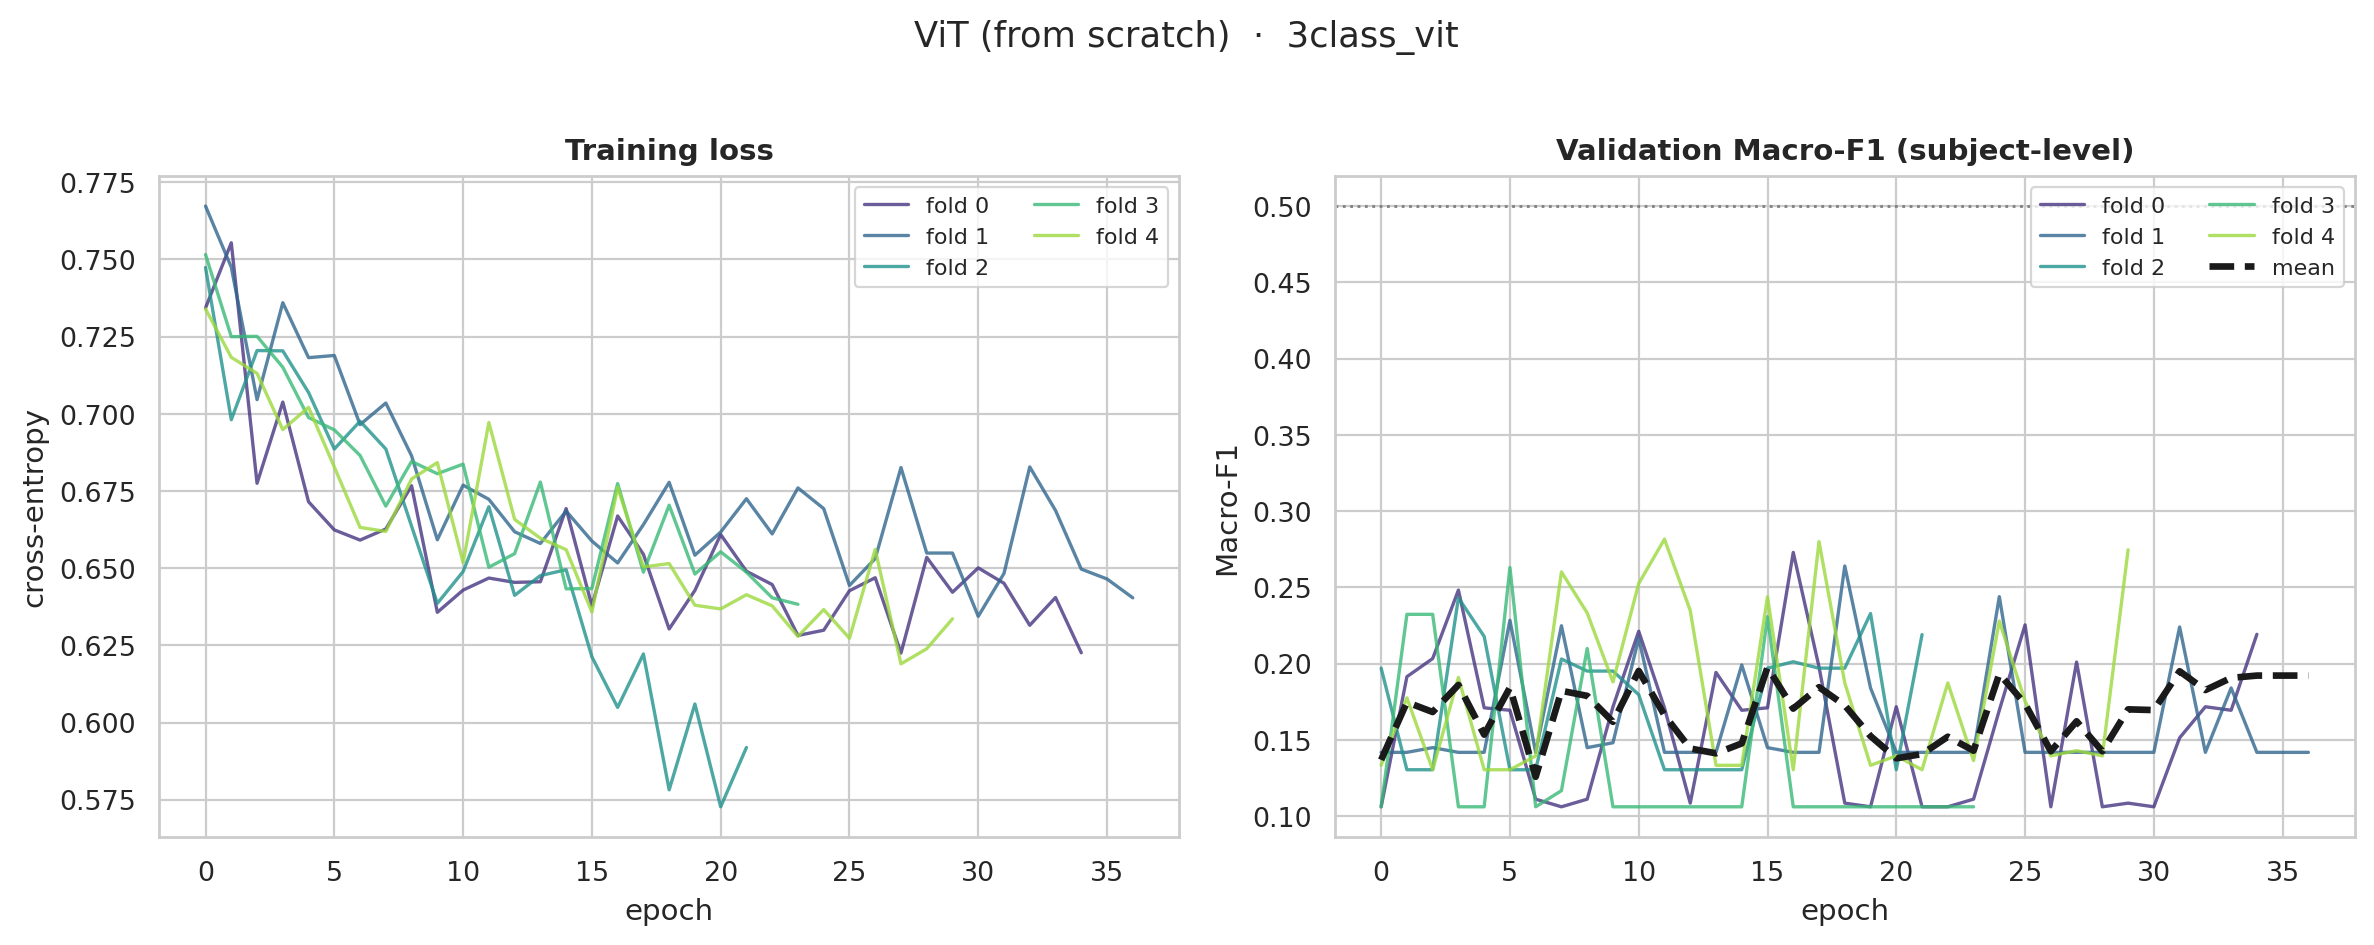
\includegraphics[width=7.6cm]{Images/tc_3class_vit.png}
    \caption[Three-class training dynamics]{\textbf{Three-class training dynamics.} DenseNet CNN (left) vs.\ from-scratch ViT (right; validation macro-F1 stays flat between about 0.1 and 0.25).}
    \label{fig:tc_vit}
\end{figure}

\section{Performance Diagnostics}
Beyond point metrics, Figure~\ref{fig:perf_extra} reports ROC, precision--recall, and calibration for the binary Swin--ViT hybrid and for the three-class CNN (one-vs-rest). The three-class one-vs-rest ROC gives AUCs of $0.69$ (CN), $0.66$ (MCI), and $0.77$ (AD): AD is the most separable class, MCI the least, and none is separated strongly --- echoing the confusion-matrix analysis.

\begin{figure}[H]
    \centering
    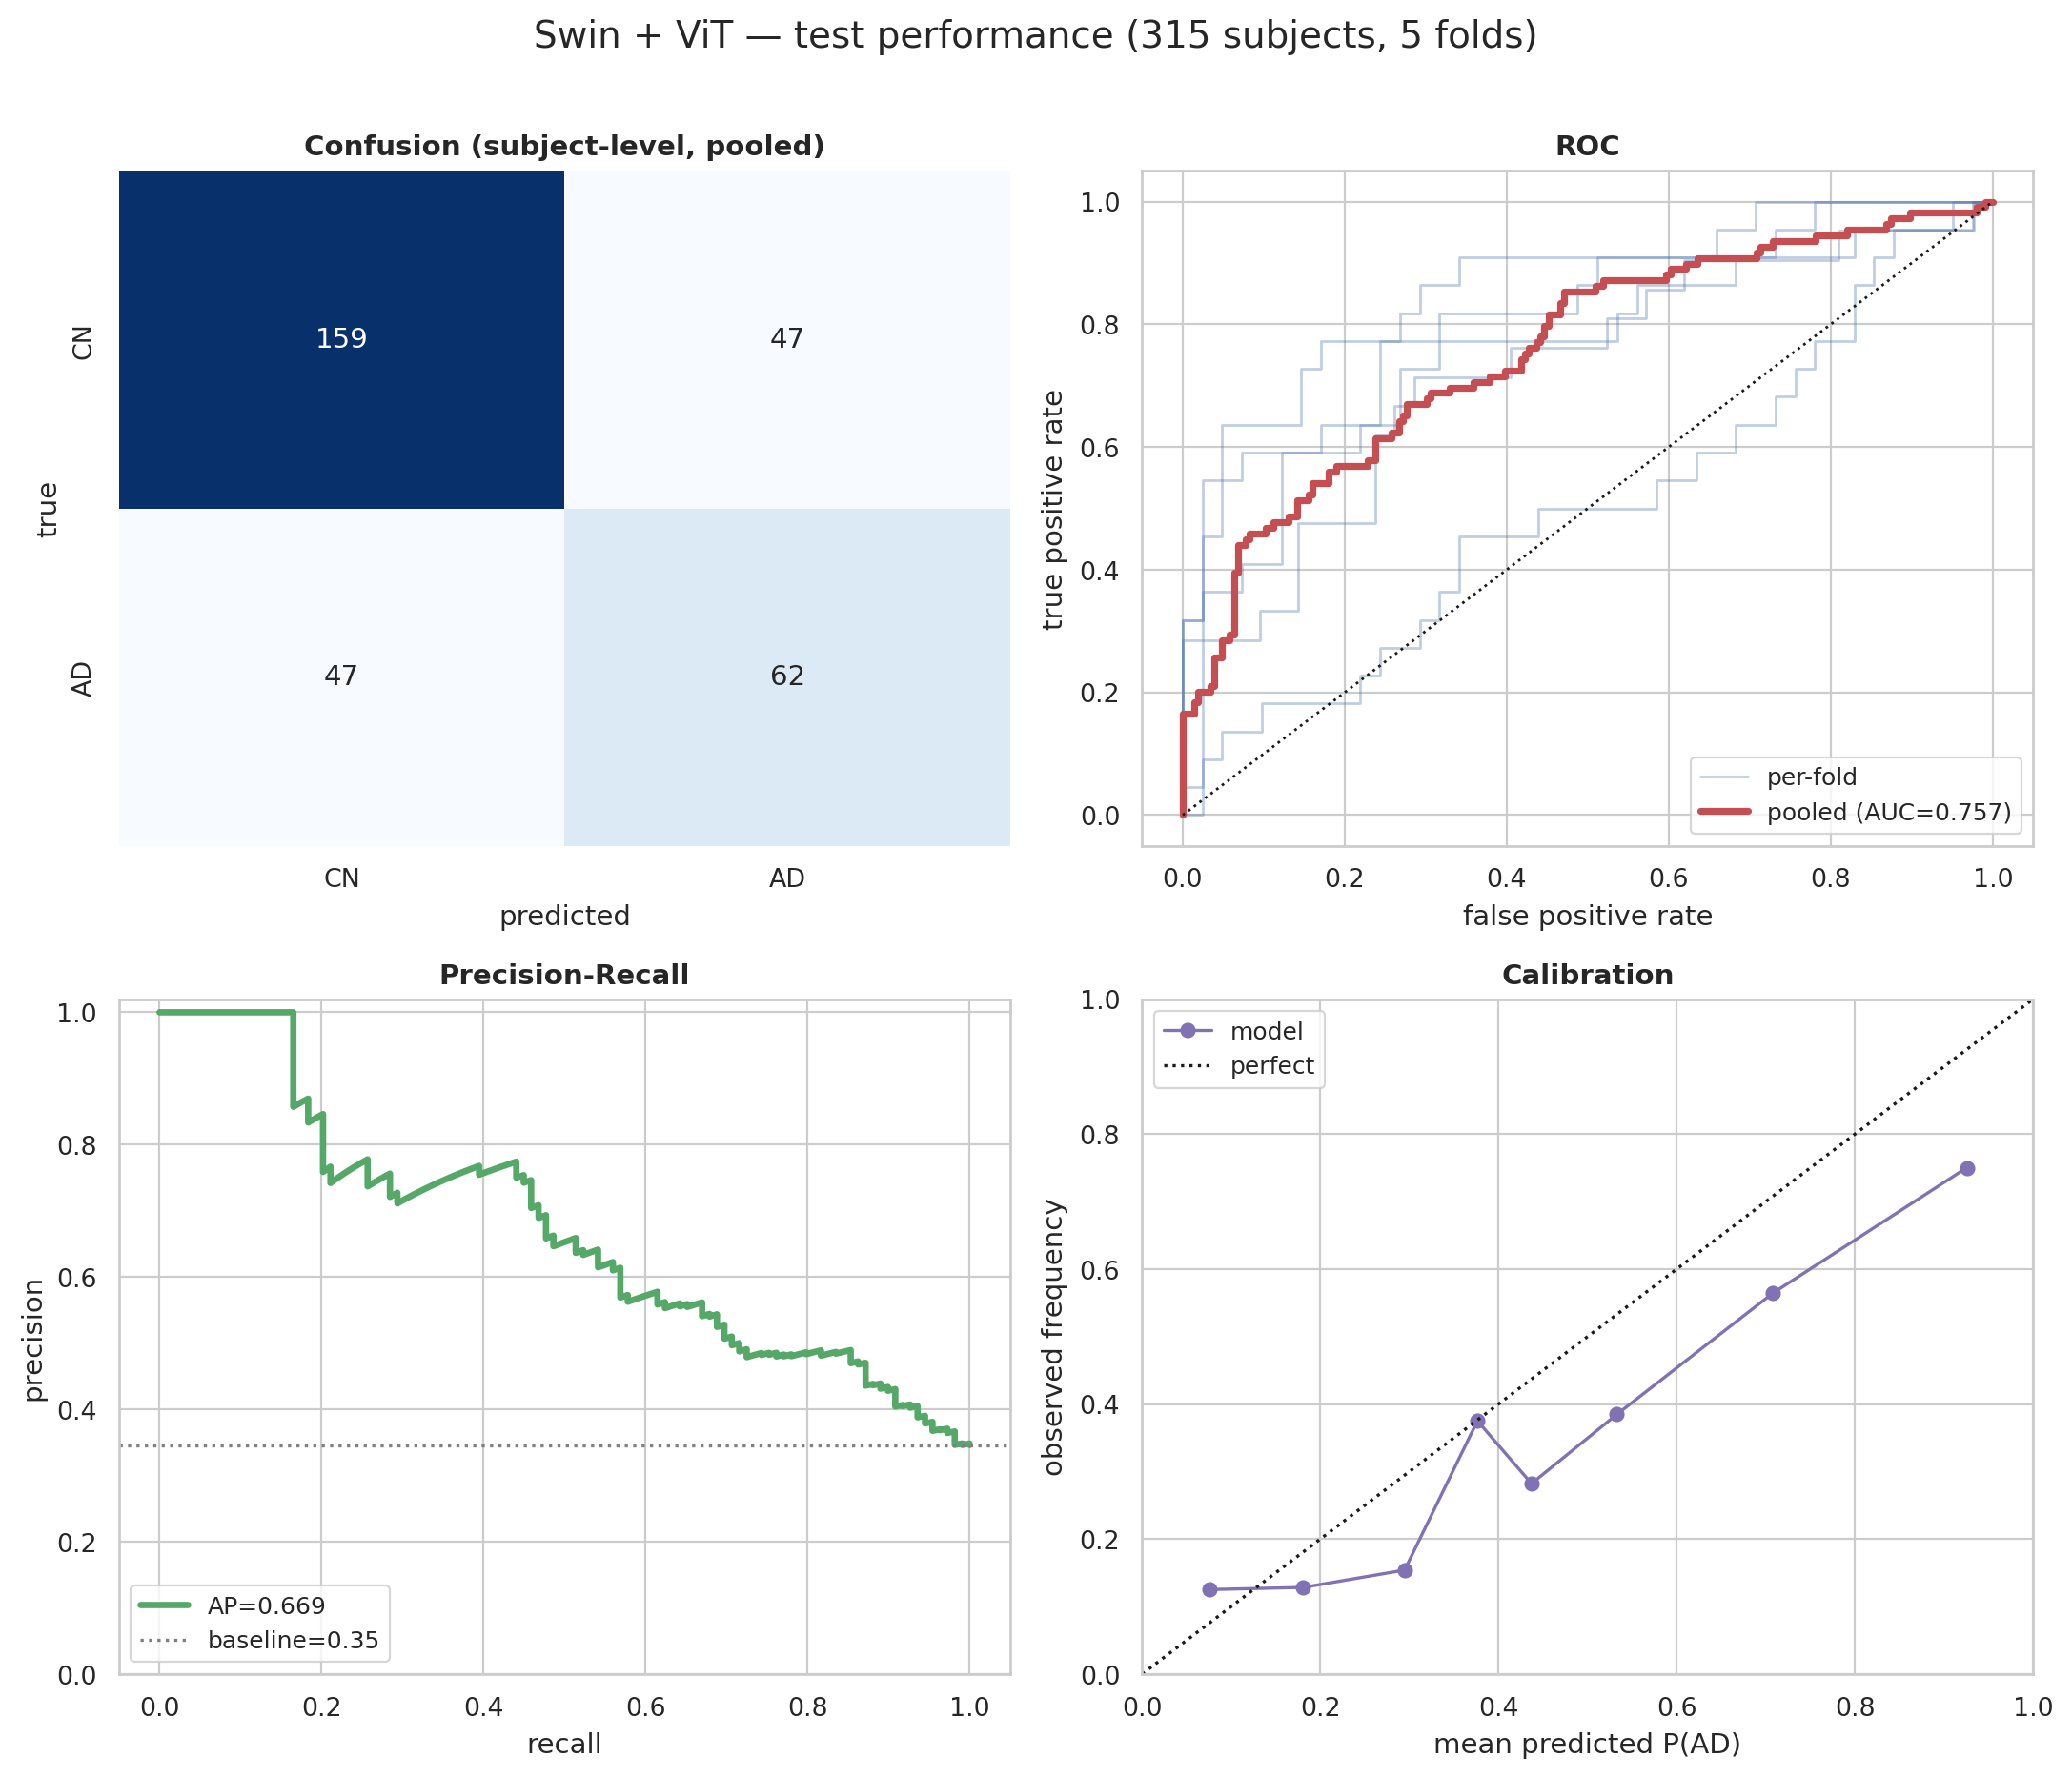
\includegraphics[width=7.6cm]{Images/perf_binary_hybrid_swinvit.png}\hfill
    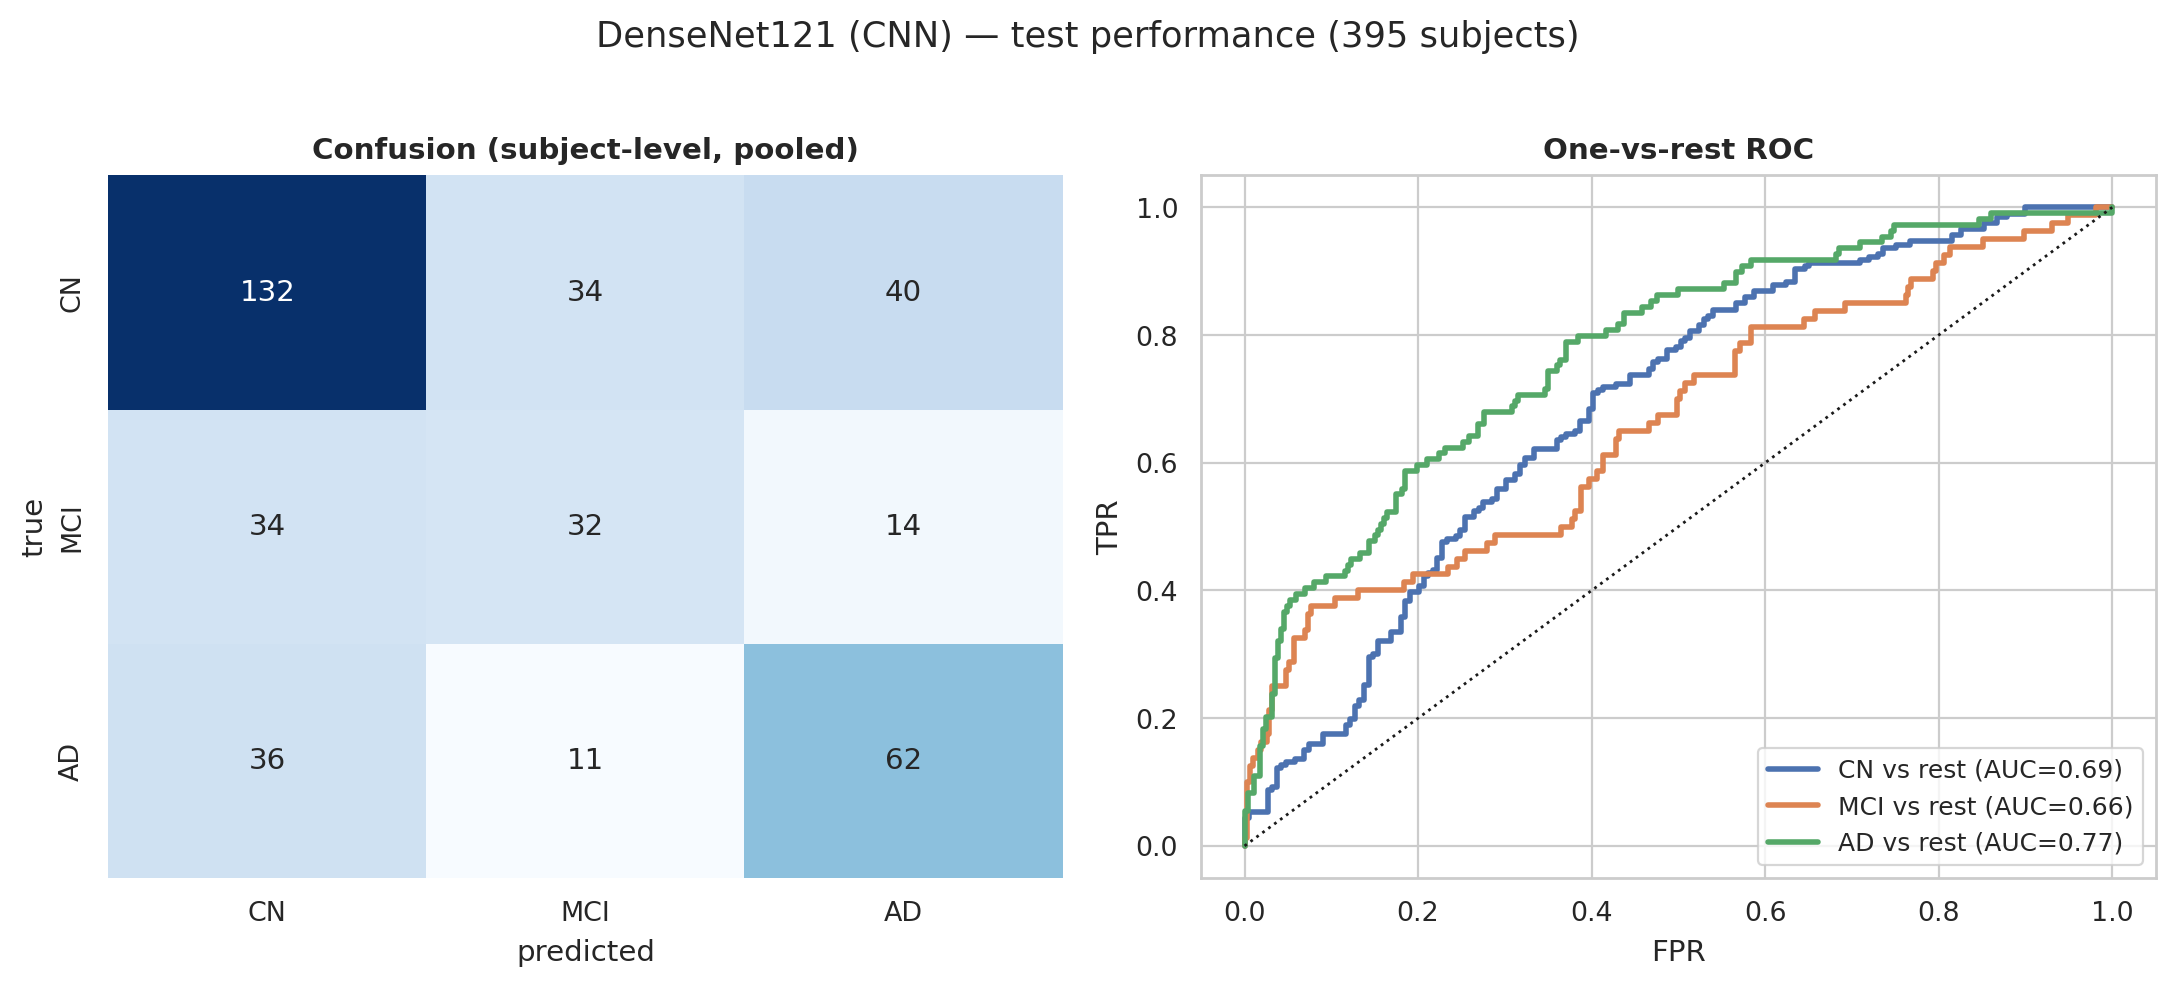
\includegraphics[width=7.6cm]{Images/perf_3class_cnn.png}
    \caption[Extended diagnostics]{\textbf{Extended diagnostics.} Binary Swin--ViT hybrid (left) and three-class CNN one-vs-rest (right).}
    \label{fig:perf_extra}
\end{figure}

\section{Feature-Space Analysis}
To see \emph{why} the models succeed or fail, Figure~\ref{fig:emb} projects the penultimate-layer features (one fold) with t-SNE. The binary CNN forms two largely separated CN/AD clusters, with the misclassified subjects concentrated in the region where they meet. For the three classes, the Swin encoder produces partially separable CN and AD regions with MCI scattered between them, whereas the from-scratch ViT produces a single undifferentiated blob --- a geometric picture of a model that never learned a useful representation.

\begin{figure}[H]
    \centering
    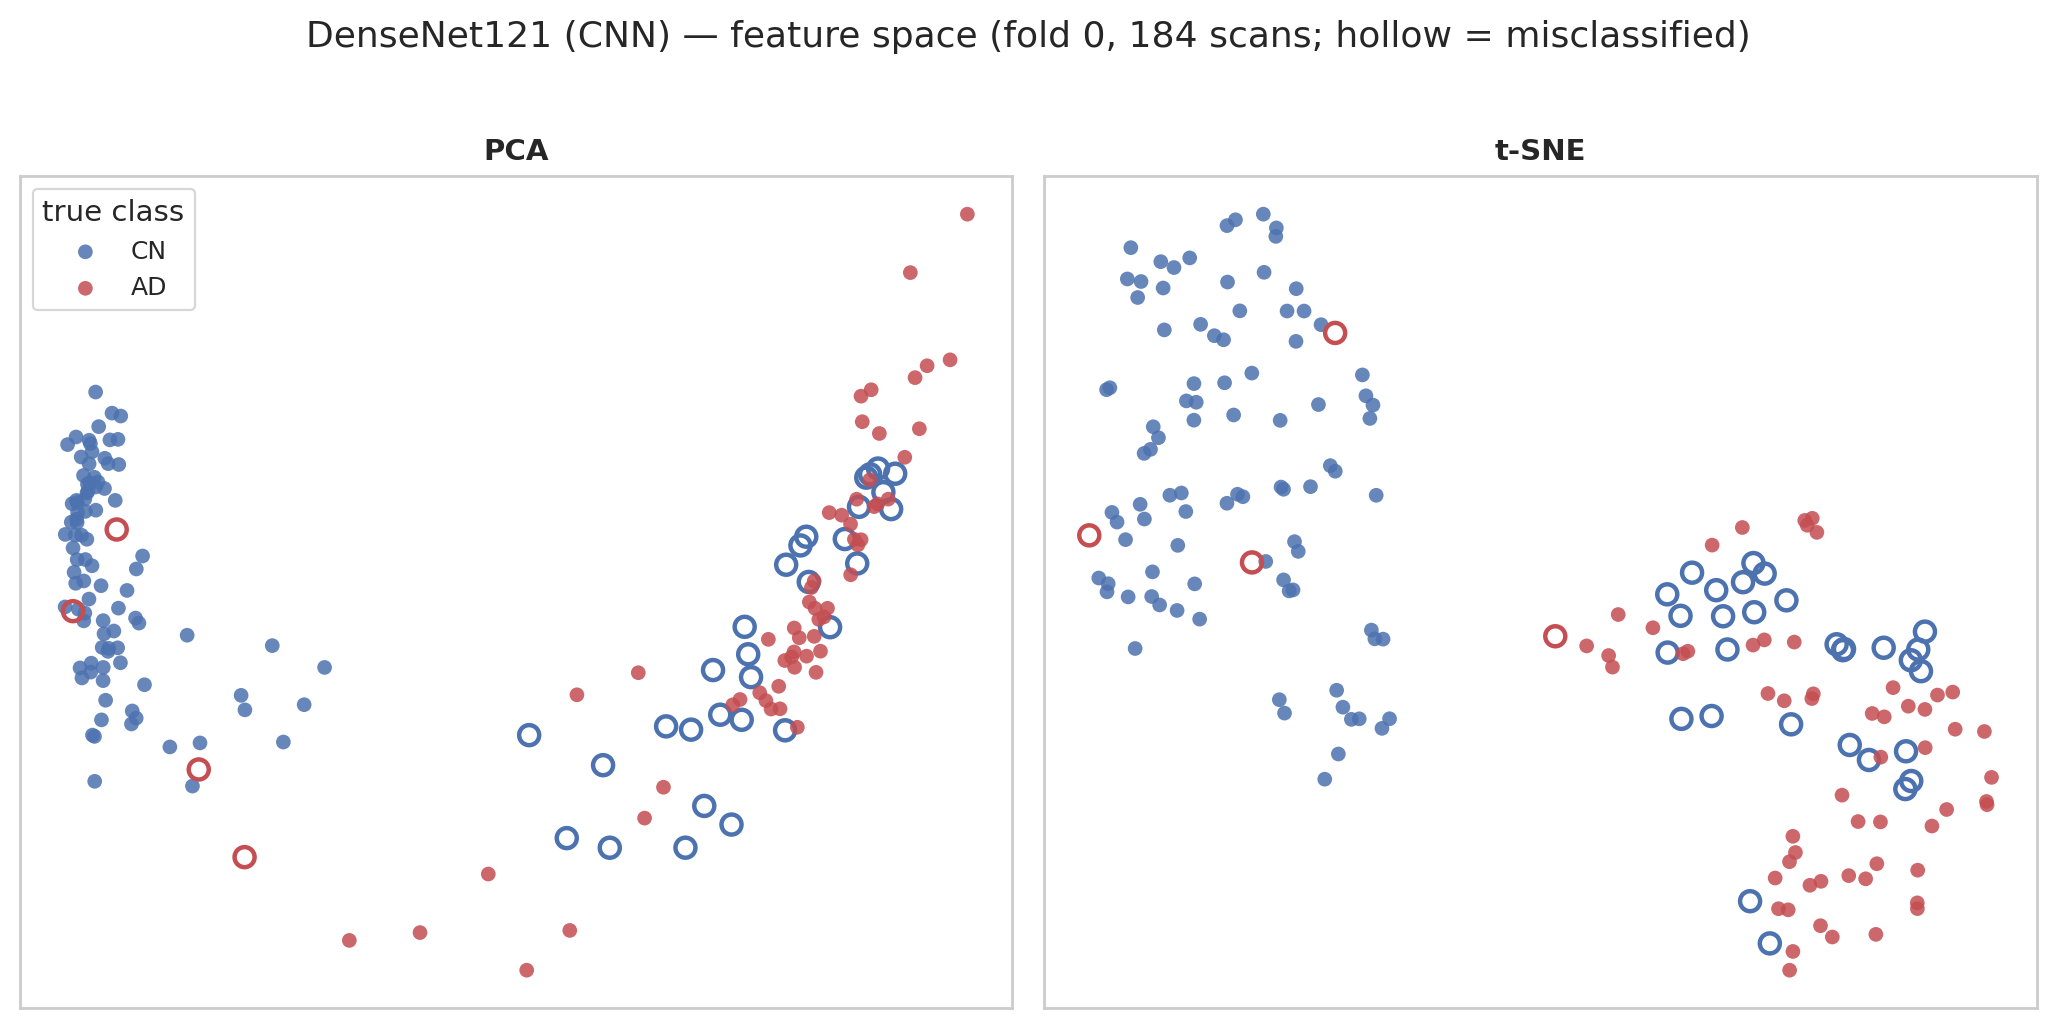
\includegraphics[width=5.1cm]{Images/emb_binary_cnn.png}\hfill
    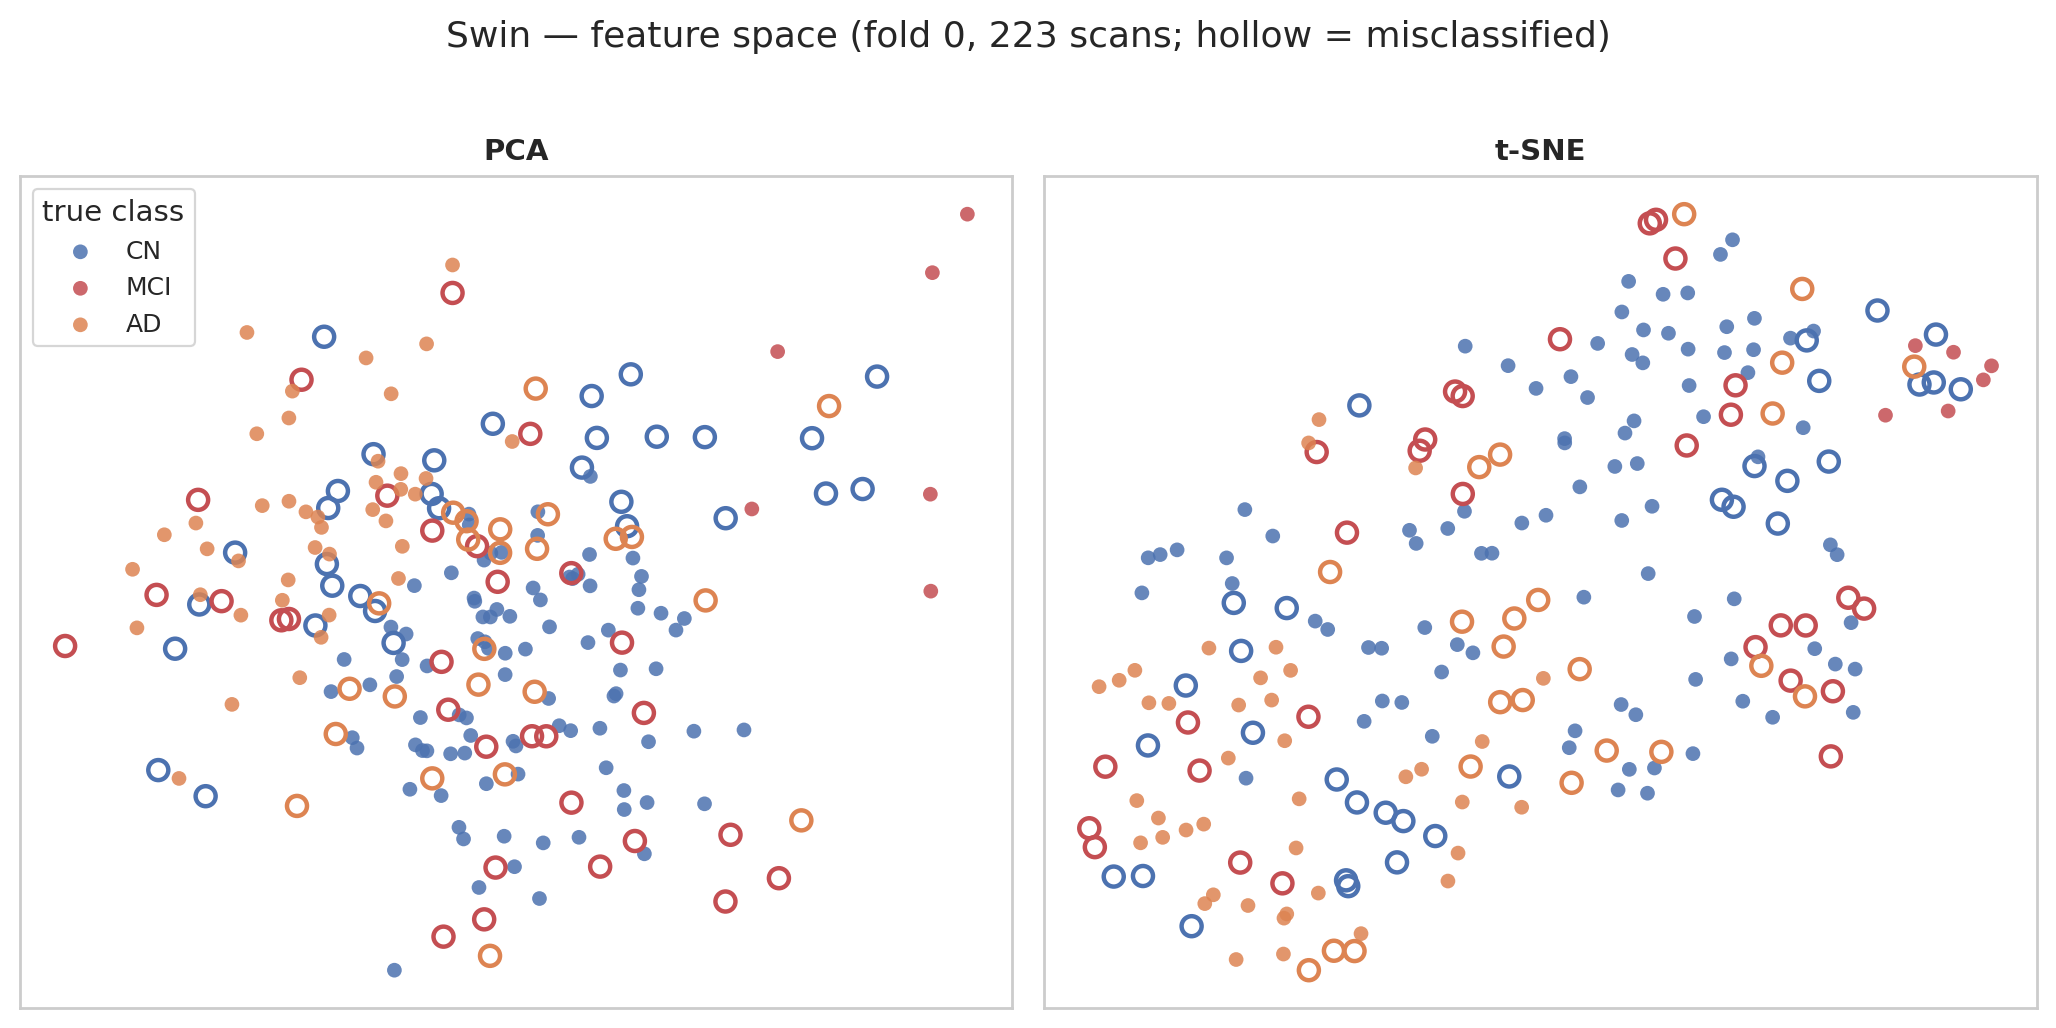
\includegraphics[width=5.1cm]{Images/emb_3class_swin.png}\hfill
    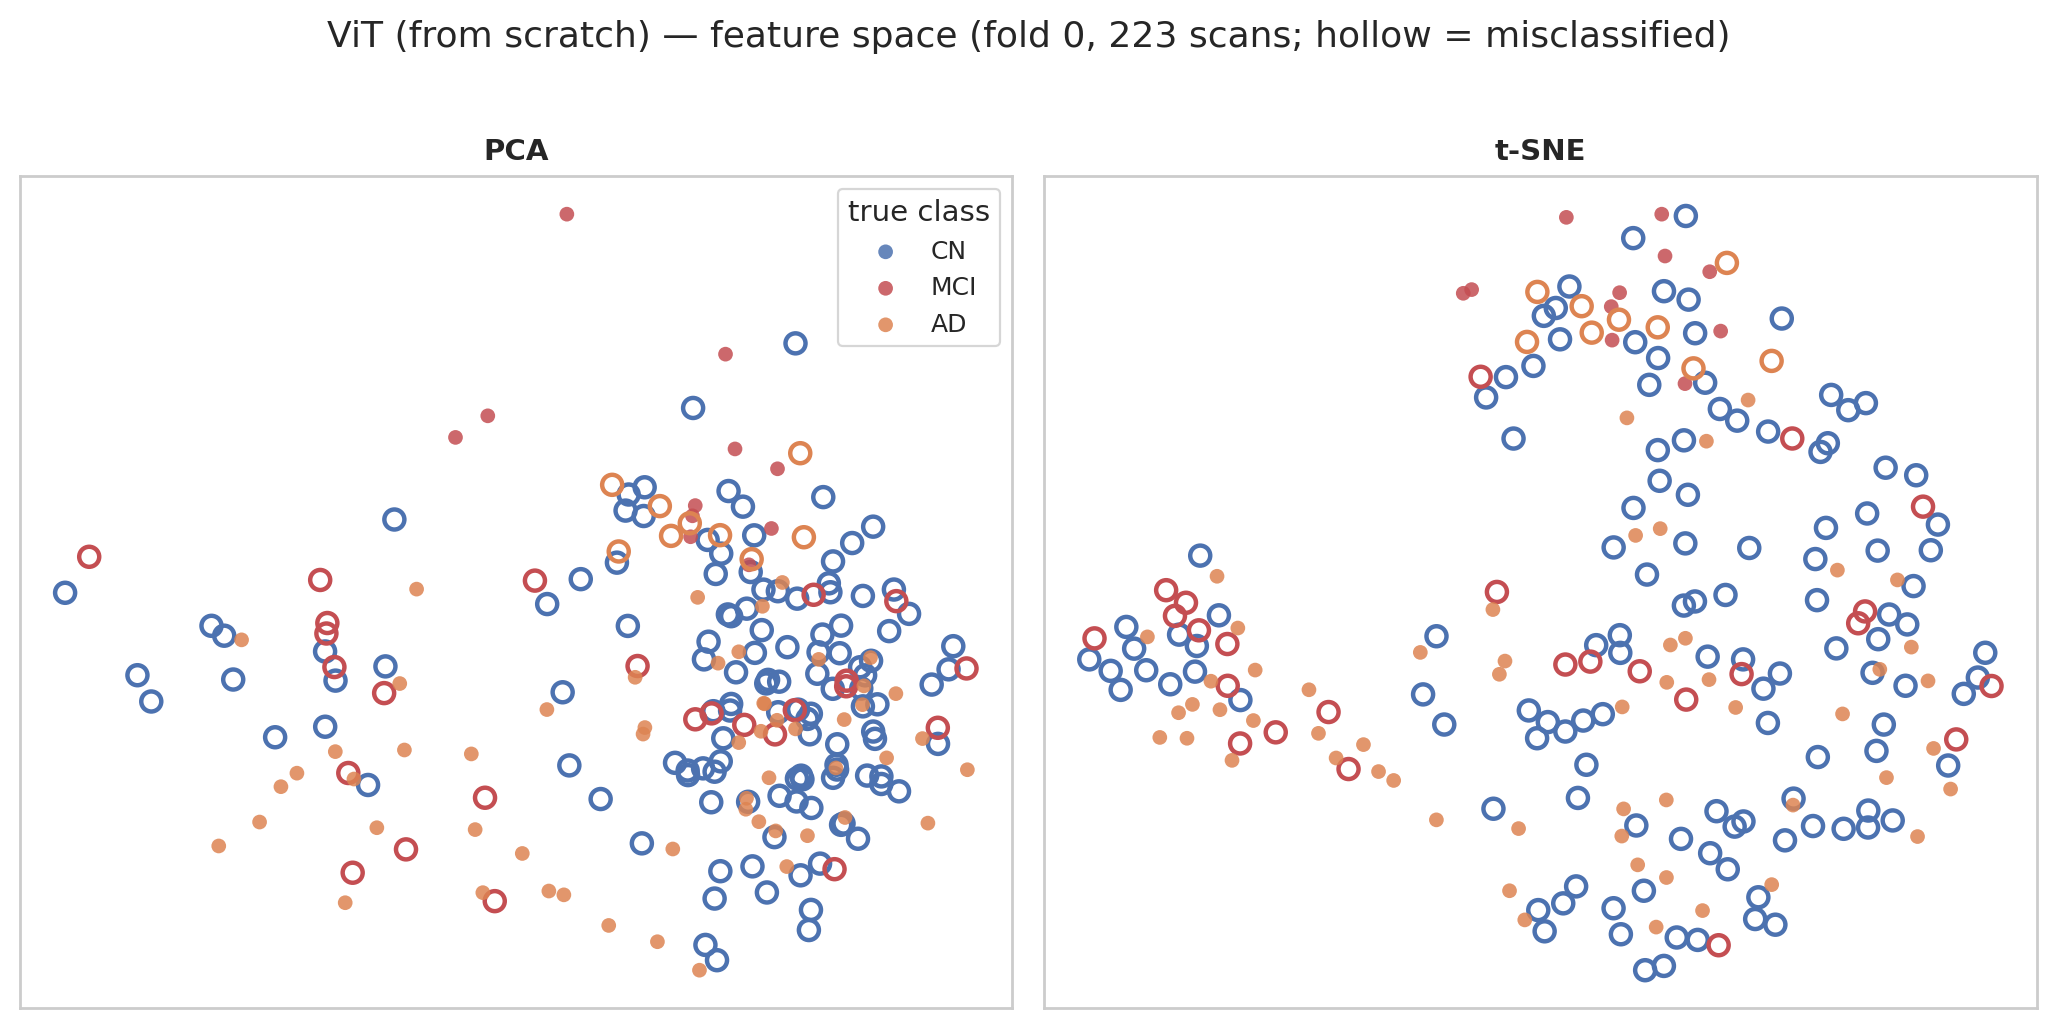
\includegraphics[width=5.1cm]{Images/emb_3class_vit.png}
    \caption[Feature embeddings]{\textbf{Feature embeddings.} t-SNE of penultimate features: binary CNN (left, two clean clusters), three-class Swin (middle, MCI between CN/AD), three-class ViT (right, collapsed).}
    \label{fig:emb}
\end{figure}

\section{Error Analysis}
Figure~\ref{fig:err} inspects the mistakes. The predicted-probability histogram by true class (three of five folds, 189 subjects) shows that many binary errors are \emph{confident}: of the 22 misclassified CN subjects, about 14 receive $P(\text{AD})>0.9$, and about 7 AD subjects receive $P(\text{AD})<0.1$. The gallery shows the most confident of these misclassifications. Confident errors of this kind are not explained by a soft decision boundary; plausible causes, still to be investigated, include label noise (for example, CN subjects who later converted), age-related atrophy in older CN subjects, and site or scanner effects. In the three-class case the per-class metrics (Table~\ref{tab:3class_perclass}) and confusion matrices show that most errors are MCI subjects assigned to CN or AD, which is consistent with MCI's intermediate clinical definition.

\begin{figure}[H]
    \centering
    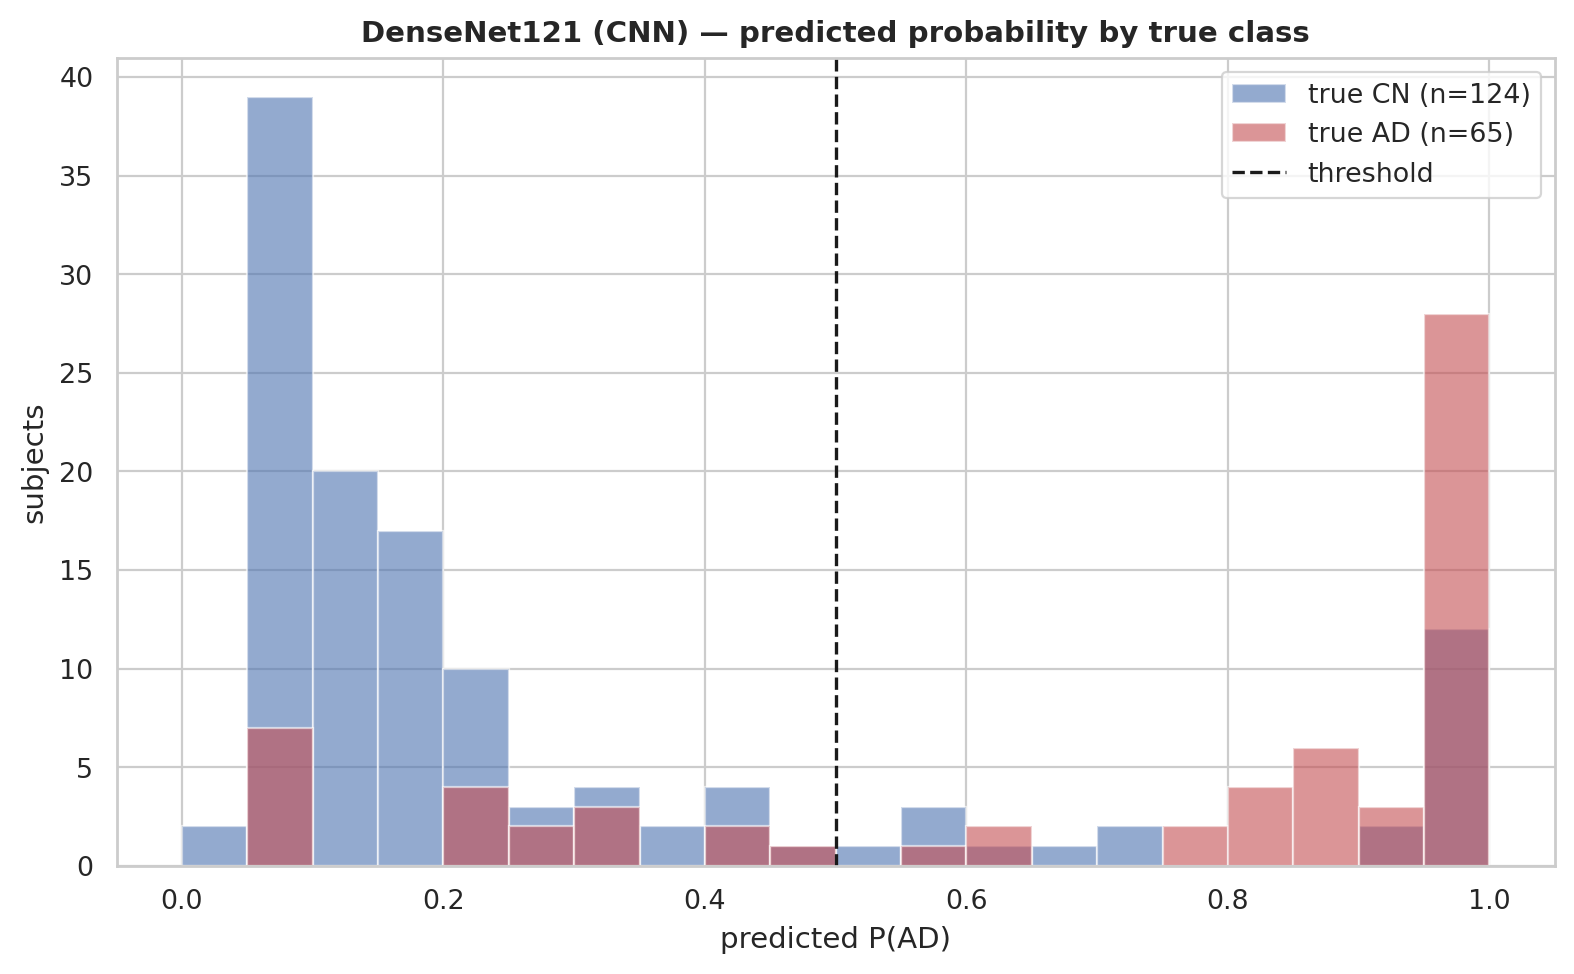
\includegraphics[width=7.6cm]{Images/err_binary_cnn_hist.png}\hfill
    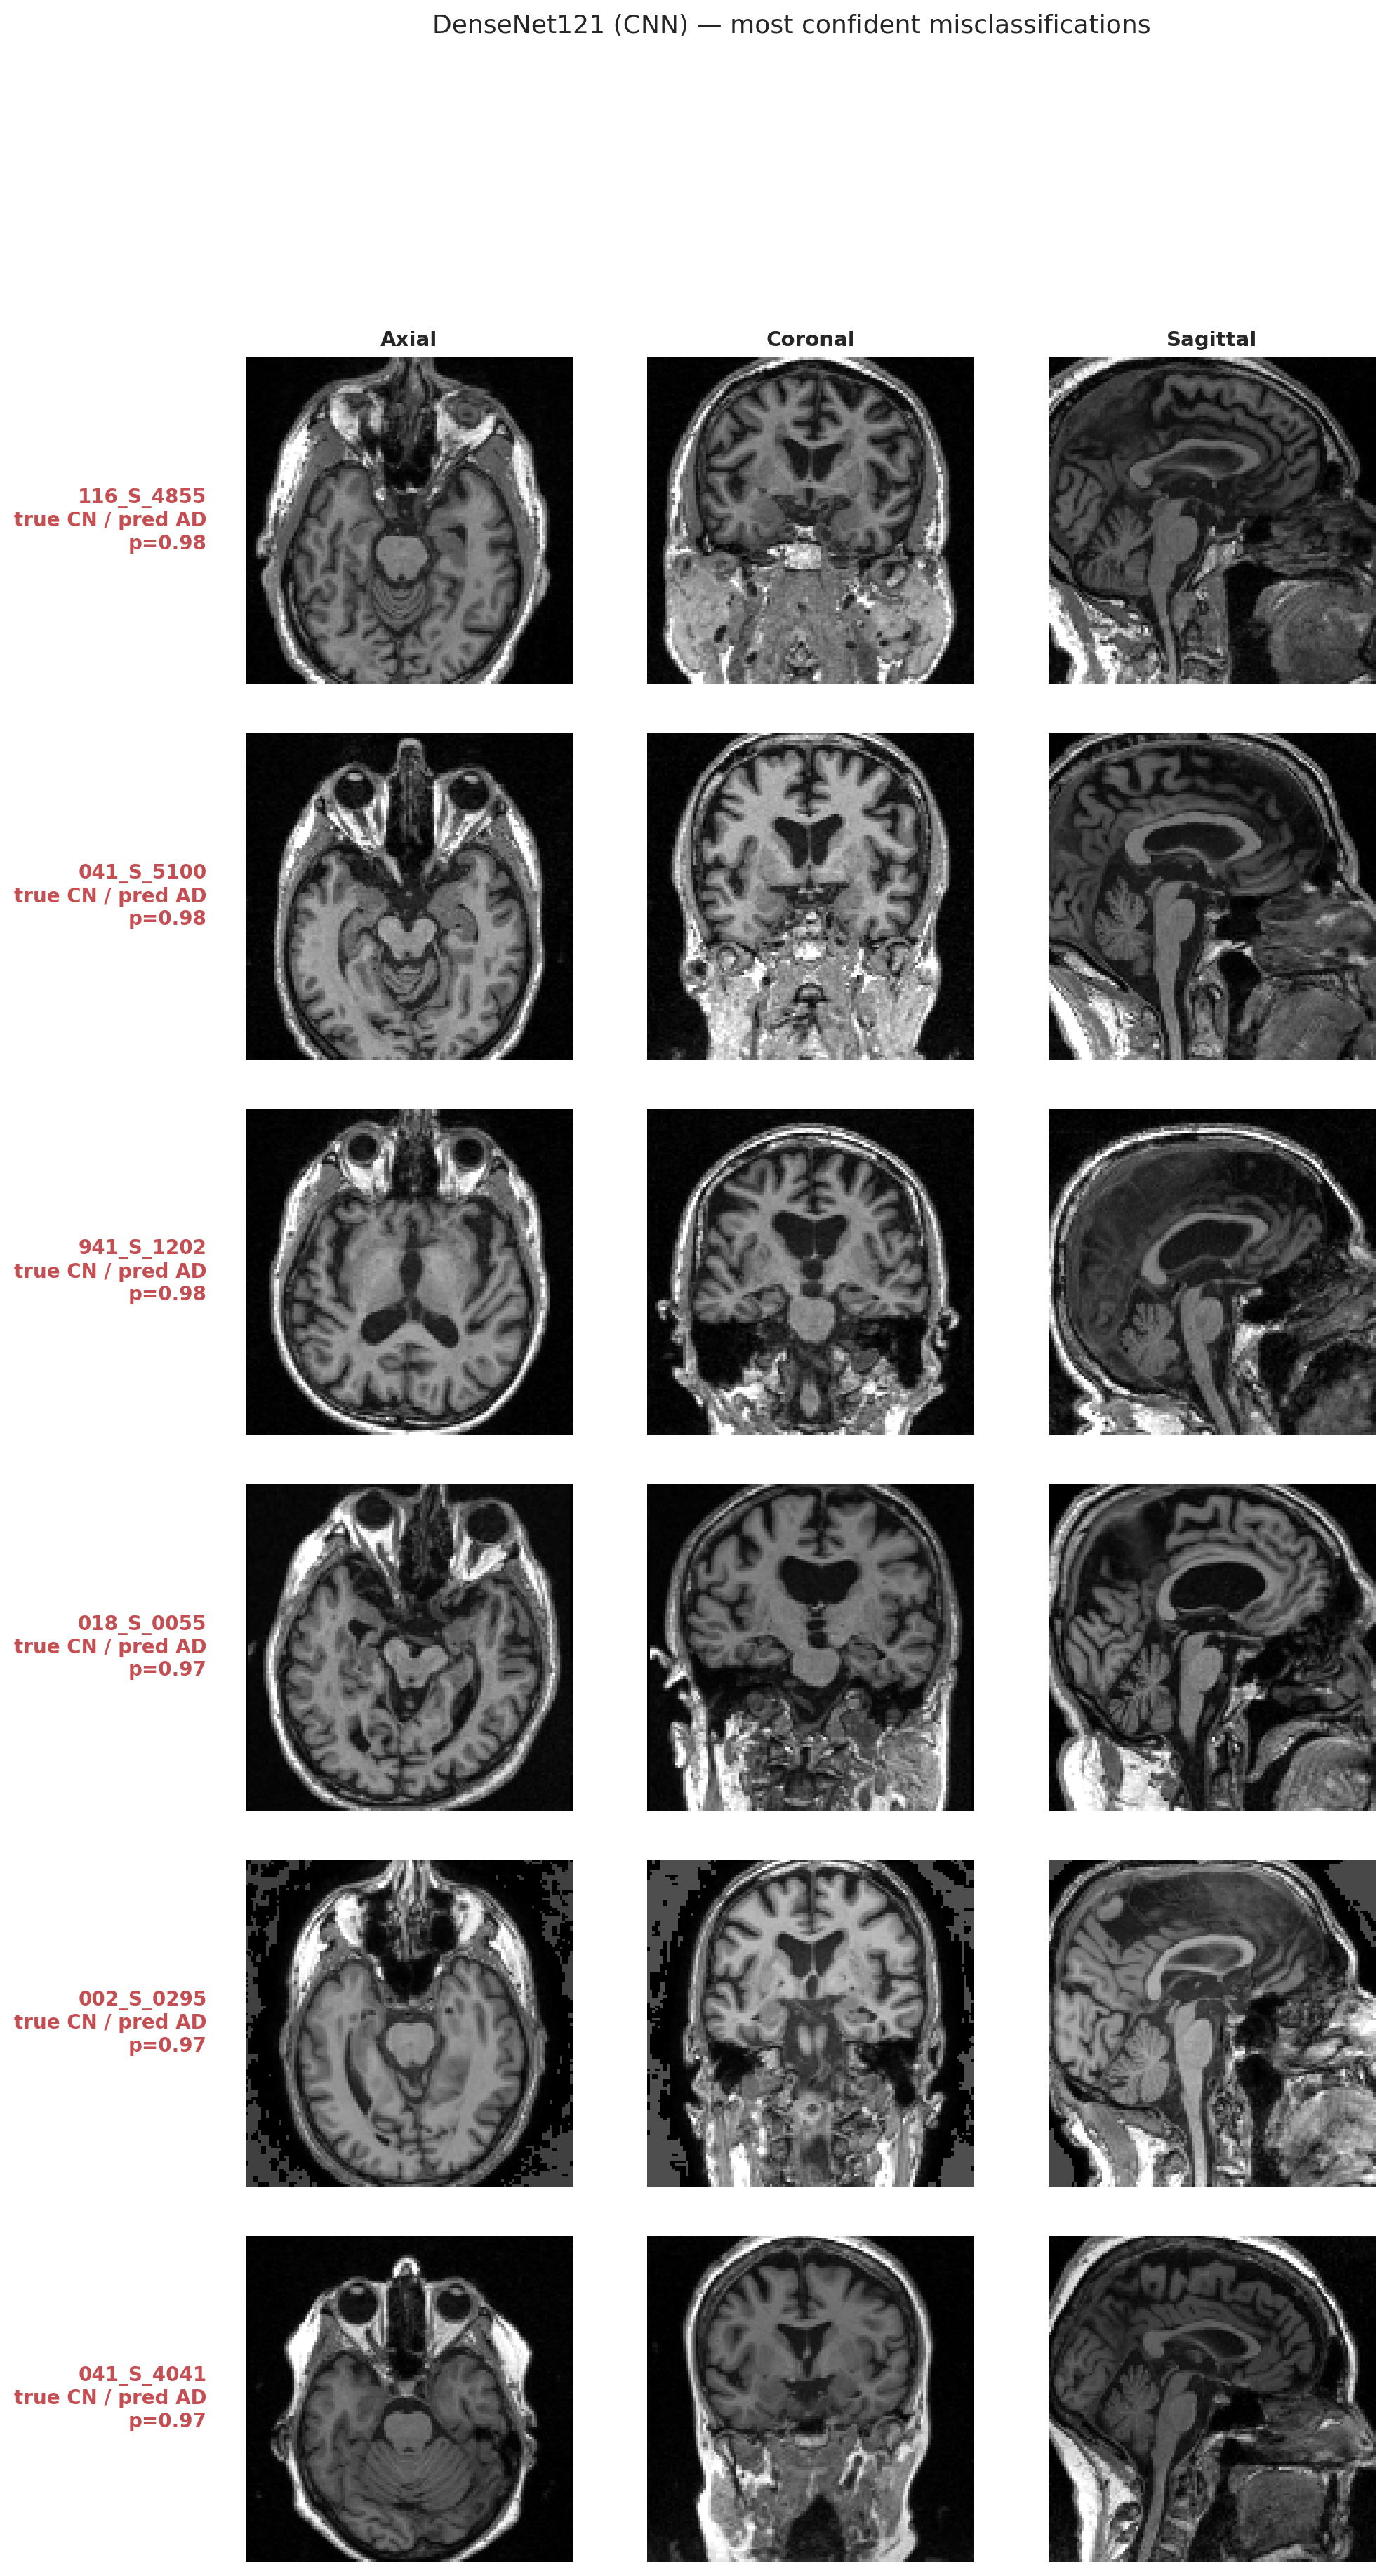
\includegraphics[width=7.6cm]{Images/err_binary_cnn_gallery.png}
    \caption[Error analysis (3 of 5 folds)]{\textbf{Error analysis (3 of 5 folds).} Binary predicted-probability histogram by true class (left) and a gallery of the most confident misclassifications (right) for the DenseNet CNN.}
    \label{fig:err}
\end{figure}

\section{Does the Hybrid Actually Help? (RQ1)}\label{sec:rq1}
The research question was whether fusing local (CNN) and global (transformer) 3D features beats either alone. The evidence is nuanced and reported honestly:
\begin{itemize}
    \item On the binary task the hybrid CNN--ViT has the highest mean, but its $+1.2$ accuracy / $+1.4$ macro-F1 margin over the standalone DenseNet is not statistically meaningful. The per-fold macro-F1 differences are $-0.052$, $+0.047$, $+0.065$, $-0.013$, and $+0.023$ (mean $+0.014$, SD $0.047$); a paired $t$-test gives $t=0.67$ with 4 degrees of freedom ($p\approx0.54$). The hybrid wins in only three of the five folds, and over all 315 subjects it classifies 259 correctly against the CNN's 255 --- a difference of four subjects.
    \item The result depends on \emph{which} branches are fused. CNN$+$ViT reaches $0.80$ macro-F1, whereas Swin$+$ViT, which has no convolutional branch, reaches $0.66$. This is consistent with the CNN branch carrying most of the signal at this data scale, but the comparison changes the first branch, not the fusion strategy, and no standalone ViT was run on the binary task, so the ViT branch's own contribution cannot be isolated.
\end{itemize}
The honest conclusion is that, on this dataset, \textbf{no improvement from hybridisation could be detected}: a well-trained 3D CNN is a very strong baseline, and adding a ViT branch leaves performance within fold-to-fold noise. A null result of this kind is a valid scientific finding, but a definitive answer to RQ1 would need standalone ViT and Swin runs on the binary task, a three-class CNN--ViT run, and repeated cross-validation with several seeds.

\section{Medical Transfer Learning: Pretrained ResNet vs. From-Scratch CNN}
Counter-intuitively, the MedicalNet-\emph{pretrained} 3D ResNet ($69.8\%$) was clearly \emph{worse} than the from-scratch DenseNet ($81.0\%$), and far less stable (std $0.139$ vs $0.041$). Our working hypothesis is that this is partly an \textbf{early-stopping artifact}. Its schedule makes a late take-off likely: the backbone is frozen for the first five epochs and then trained at a 10$\times$ lower learning rate ($10^{-5}$), while early stopping uses the shortest patience of any model (12 epochs). Three of the five folds are competitive while two stop before recovering. The two weak folds score an identical $0.449$, which is itself unusual and should be checked against the saved predictions. This hypothesis has not been tested here --- the per-fold ResNet curves are not shown, and the run was not repeated with a minimum-epoch guard before early stopping. The result should therefore be read as a property of the training schedule as much as of the architecture, not as evidence that medical pretraining is useless.

\section{Why the From-Scratch ViT Collapses}\label{sec:vit_collapse}
The pure 3D ViT reaches only $28.6\%$ on the three-class task, with almost no fold variance. This is not ``chance'' in the useful sense: it is far \emph{below} the $52.2\%$ obtained by always predicting the majority class. Its confusion matrix shows why --- the model \textbf{never predicts CN} and splits every subject between MCI and AD, and its training loss barely decreases. Two factors plausibly combine here. The first is the expected weakness of a data-hungry, low-inductive-bias transformer trained from scratch on a few hundred subjects, which is why the literature relies on large-scale pretraining for ViTs~\cite{dosovitskiy2021image}. The second is that the imbalance corrections (class weighting, weighted sampling, and focal loss) push a model that has learned nothing useful towards the minority classes; when several are active at once they can over-correct. Separating the two would require re-running the ViT with a single imbalance correction. Reported as a negative result, it supports pairing the transformer with a CNN, which supplies the missing inductive bias, rather than using a transformer alone.

\section{Explainability Analysis (RQ2)}
To test whether the models attend to anatomically meaningful regions, a suite of 3D attribution methods was applied (Grad-CAM, Grad-CAM++, Integrated Gradients, SmoothGrad, Occlusion, and attention rollout for the transformer branch)~\cite{selvaraju2017gradcam,sundararajan2017axiomatic,abnar2020quantifying}. Figure~\ref{fig:xai_panel} shows the method-comparison panel for the DenseNet CNN on one AD subject (\texttt{135\_S\_4863}, an axial slice at the level of the lateral ventricles). \textbf{The methods do not agree.} Grad-CAM highlights the frontal region; Grad-CAM++ and Score-CAM highlight a central, peri-ventricular area; occlusion responds mainly to the occipital region and the back of the skull; LIME includes part of the scalp; and Integrated Gradients is nearly empty on this slice.

\begin{figure}[H]
    \centering
    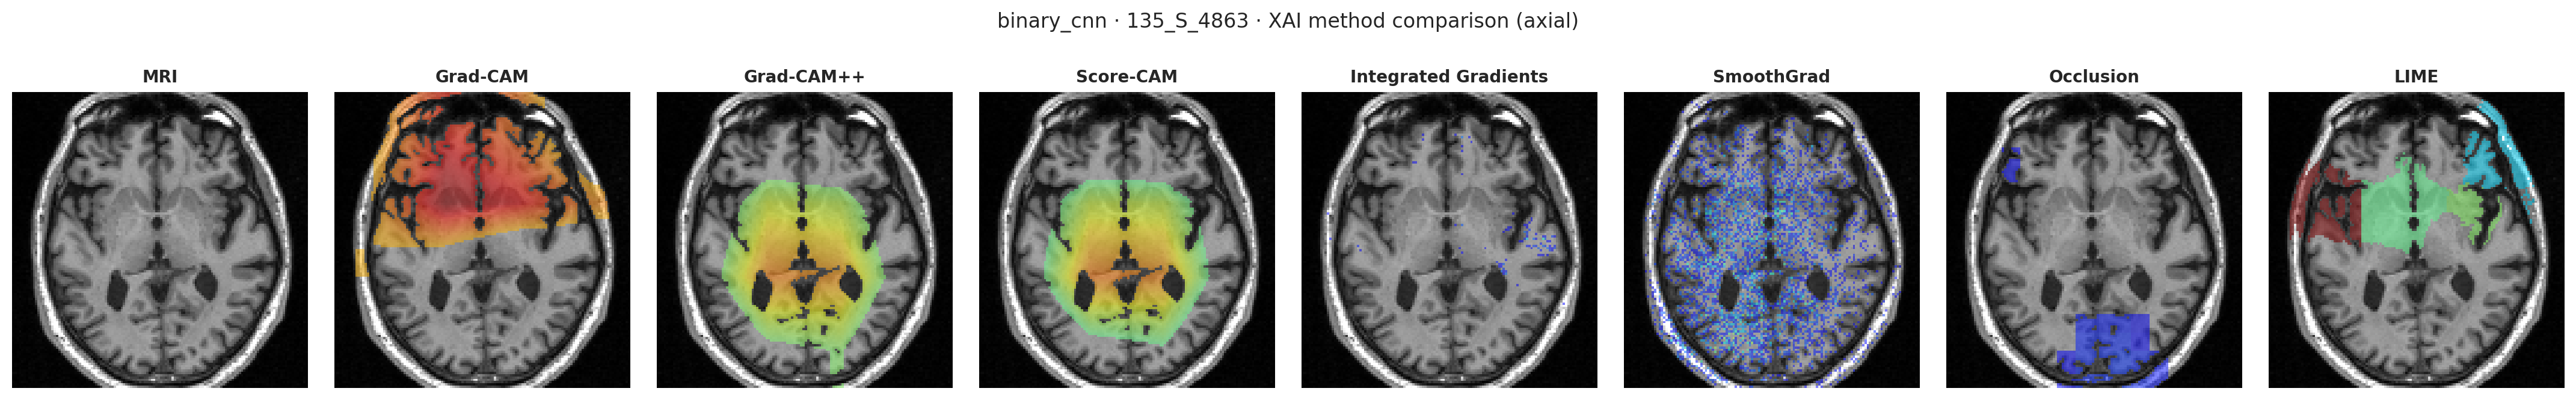
\includegraphics[width=15cm]{Images/xai_panel_binary_cnn.png}
    \caption[XAI method comparison]{\textbf{XAI method comparison.} Explainability for the binary DenseNet CNN on one AD subject: Grad-CAM, Grad-CAM++, Score-CAM, Integrated Gradients, SmoothGrad, Occlusion, and LIME. The methods highlight different regions, including non-brain tissue.}
    \label{fig:xai_panel}
\end{figure}

Because the hybrid CNN--ViT checkpoints were not retained, \textbf{no explanation maps exist for the proposed model}; the per-subject maps above use the standalone DenseNet, which is statistically tied with it. The group-level regional analysis (Figure~\ref{fig:xai_roi}) was computed for a different model, the binary \emph{Swin--ViT} hybrid, over 16 AD subjects from a single fold. It splits the volume into thirds along each axis. The result is close to uniform (all nine values lie between $0.036$ and $0.055$): on the left--right axis the \emph{middle} third is the \emph{lowest}, and the posterior and inferior thirds receive slightly more importance than the anterior and superior thirds. This does not show a concentration on medial or central structures.

\begin{figure}[H]
    \centering
    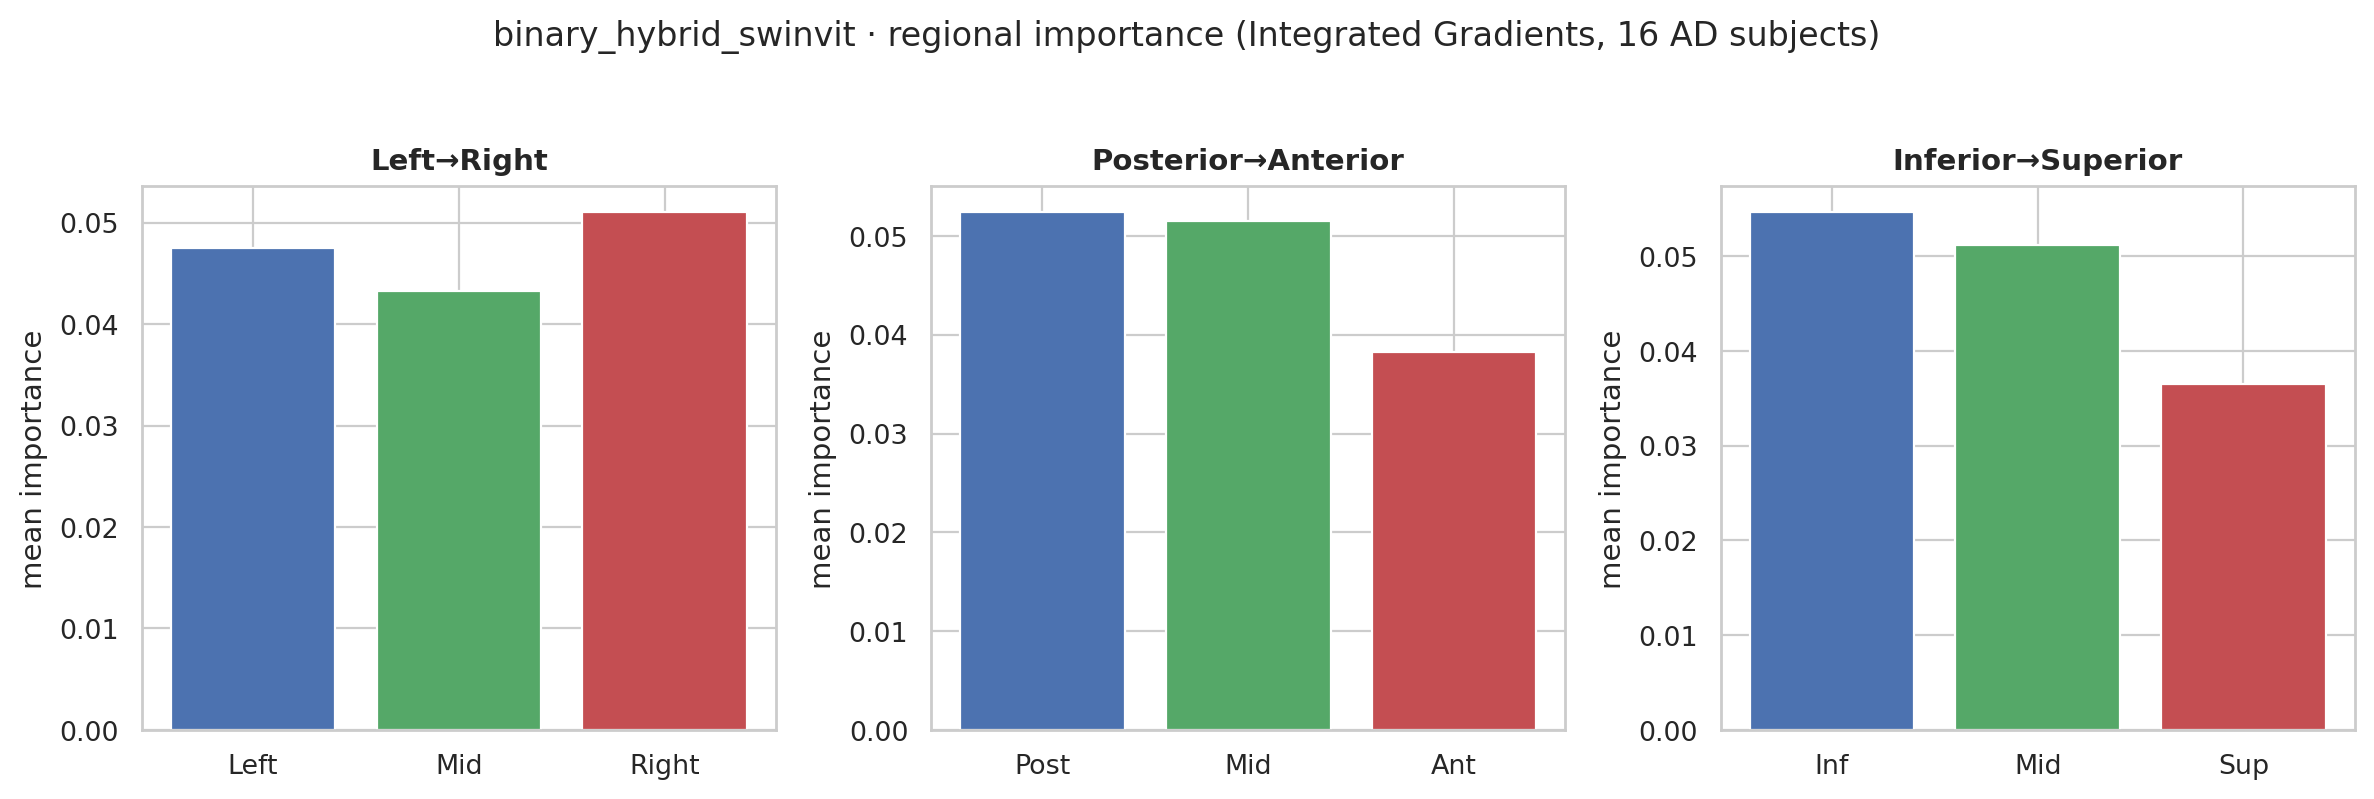
\includegraphics[width=13cm]{Images/xai_roi_binary.png}
    \caption[Group-averaged importance (Swin--ViT)]{\textbf{Group-averaged importance (Swin--ViT hybrid, 16 AD subjects, one fold).} Mean Integrated-Gradients importance over spatial thirds of the head volume. \textbf{Honesty note:} the ADNI volumes are not skull-stripped or atlas-registered, so these are coarse thirds of the head volume, not anatomical ROIs.}
    \label{fig:xai_roi}
\end{figure}

Taken together, these maps do \emph{not} yet establish that the models rely on AD-relevant anatomy. Because the skull, scalp, orbits, and neck are still present in the input, a model could exploit non-brain cues, and several methods do place importance there. Establishing anatomical grounding would require skull-stripping, registration to an atlas so that importance can be summed over named ROIs such as the hippocampus, and sanity checks such as model-randomisation tests and deletion curves.

Figure~\ref{fig:xai_hybrid} shows the panel for the Swin--ViT hybrid, including \textbf{attention rollout} from the transformer branch. On this inferior slice, attention rollout falls near the orbit and skull base, Grad-CAM falls largely on the scalp and posterior neck, and occlusion highlights the cerebellum. Figure~\ref{fig:xai_3class} shows the three-class Swin panel and its group-averaged Integrated Gradients over 16 correctly classified AD subjects. The per-subject Grad-CAM again responds to extra-cerebral tissue (temporal muscle and orbits) as well as the cerebellum, and the group-averaged attribution is diffuse --- spread across the cortex, cerebellum, brainstem, and scalp rather than focused on the medial temporal lobe. These maps are reported for transparency; they are not evidence of disease-specific localisation.

\begin{figure}[H]
    \centering
    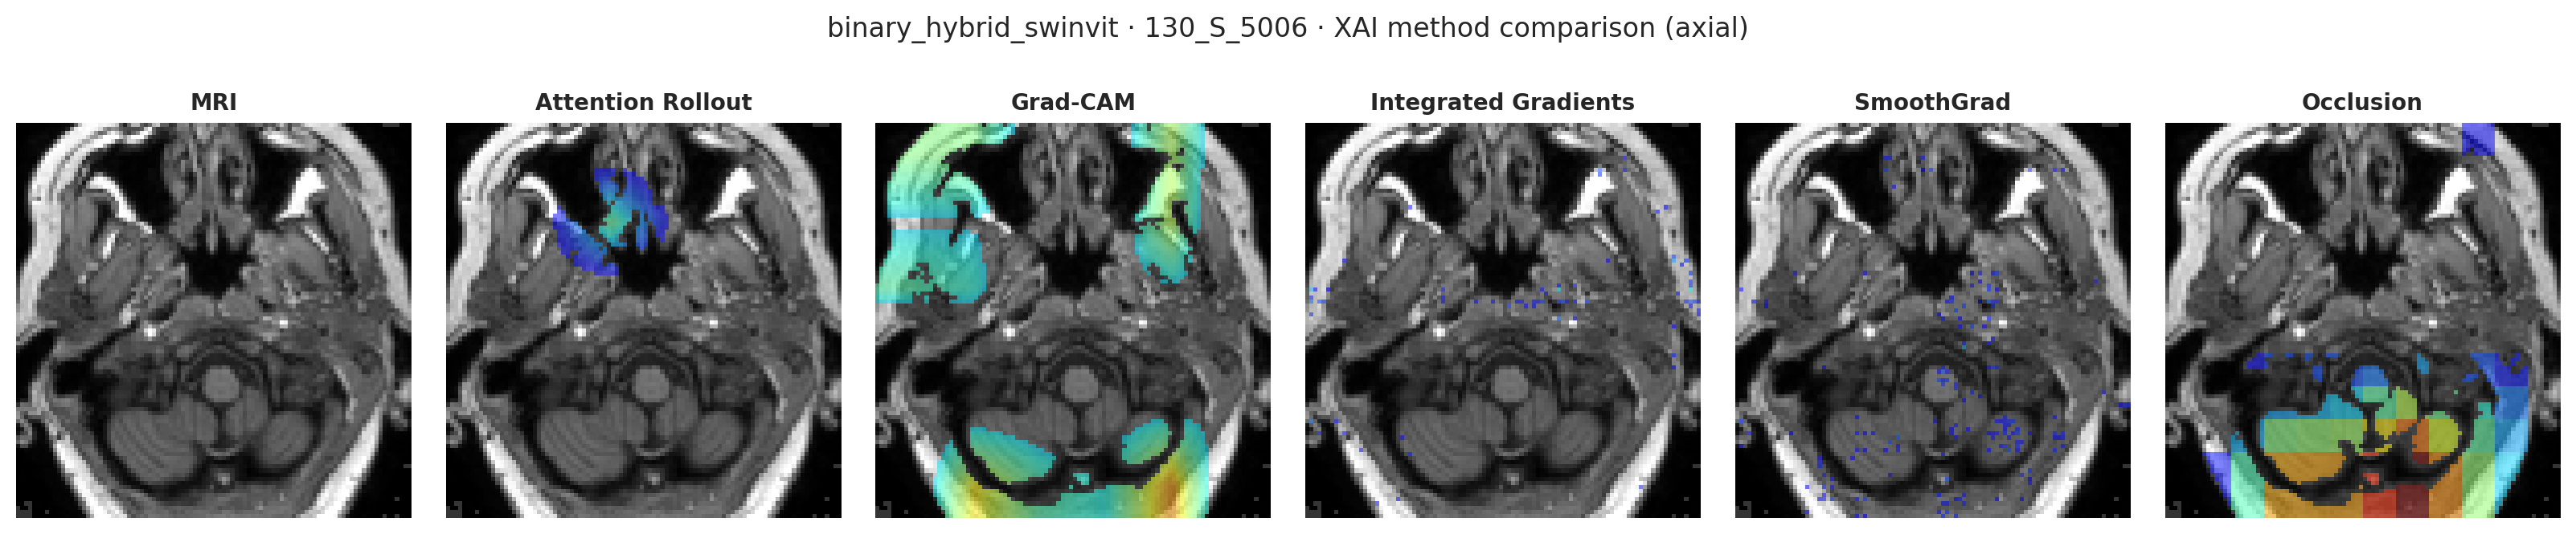
\includegraphics[width=15cm]{Images/xai_panel_hybrid.png}
    \caption[Swin--ViT hybrid explainability]{\textbf{Swin--ViT hybrid explainability.} Panel for the binary Swin--ViT hybrid (not the proposed CNN--ViT), including transformer attention rollout alongside Grad-CAM, Integrated Gradients, SmoothGrad, and occlusion.}
    \label{fig:xai_hybrid}
\end{figure}

\begin{figure}[H]
    \centering
    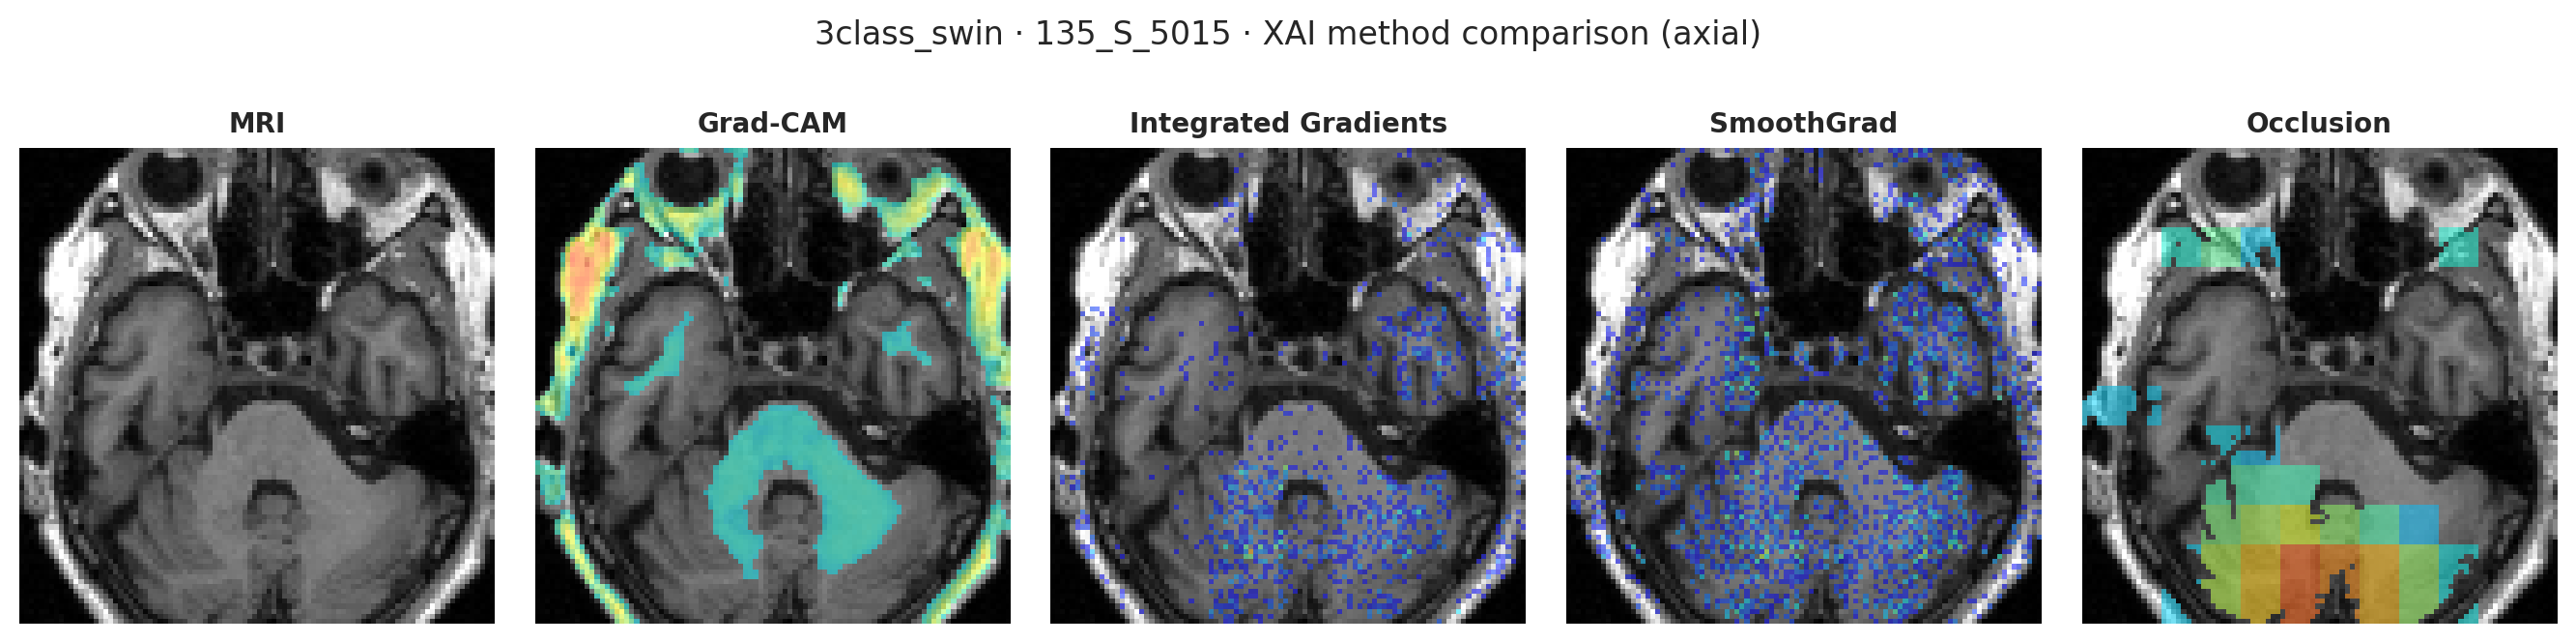
\includegraphics[width=10.5cm]{Images/xai_panel_3class_swin.png}\\[4pt]
    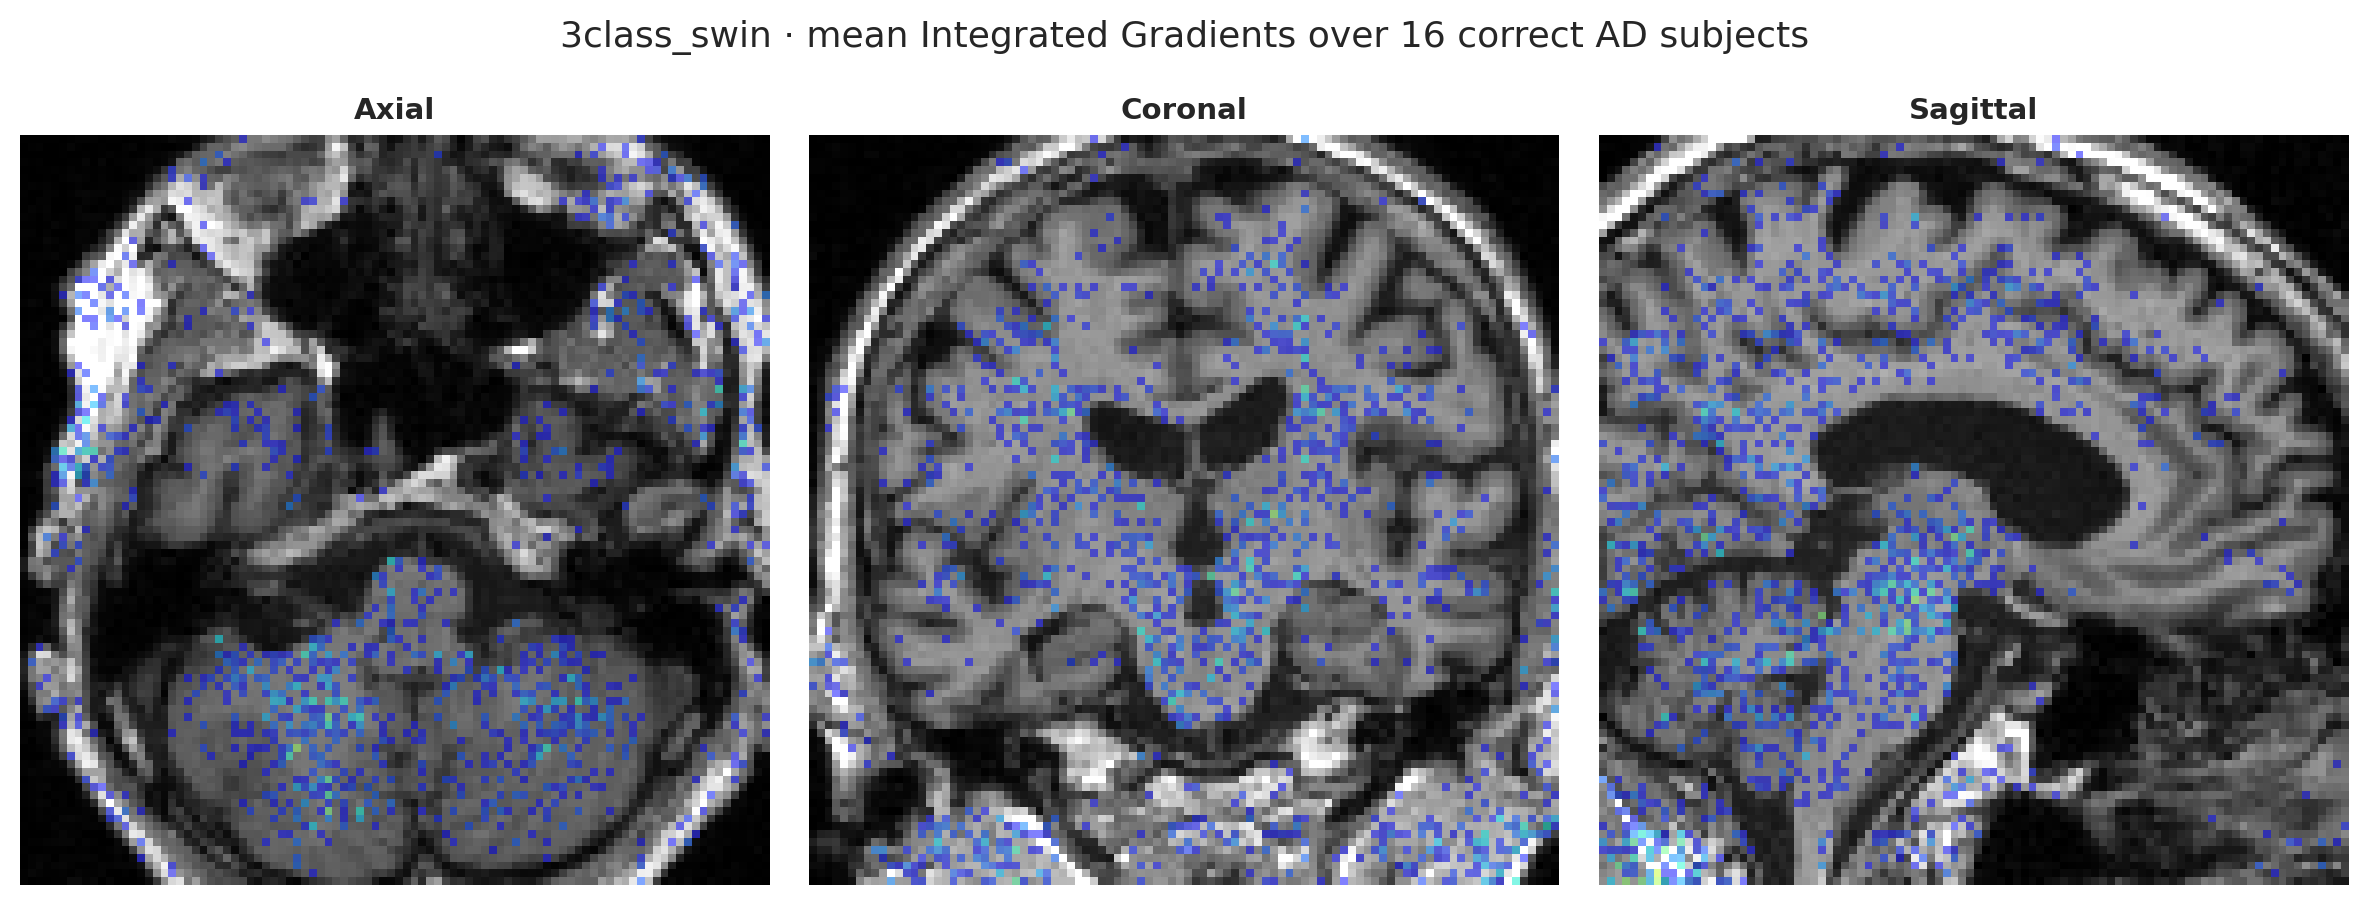
\includegraphics[width=12cm]{Images/xai_groupavg_3class.png}
    \caption[Three-class explainability]{\textbf{Three-class explainability.} Swin per-subject method panel (top) and group-averaged Integrated-Gradients importance (bottom).}
    \label{fig:xai_3class}
\end{figure}

\section{Comparison with the Literature}
Table~\ref{tab:compare_lit} places these results against the accuracies surveyed in Chapter~\ref{cha:LiteratureReviewU}. Many reported systems exceed $98\%$, but almost all split the data at the level of 2D slices (or use the curated Kaggle 2D set), which leaks a patient's slices across train and test and inflates accuracy~\cite{wen2020convolutional,yagis2021effect}. Studies that evaluate whole 3D volumes at the subject level report far more modest numbers: Wen \etal~\cite{wen2020convolutional} obtain $85$--$88\%$ for AD-vs-CN with subject-level 3D CNNs, and the ROI-based 3D ViT ensemble~\cite{saoud2024explainable}, which uses one baseline scan per subject, reports $90\%$ for AD-vs-CN and only $60\%$ for three-class. This work's $82\%$ (binary) and $58\%$ (three-class, Swin) lie in the same regime, but somewhat \emph{below} these subject-level references. The gap is plausibly explained by the absence of skull-stripping and registration, the reduced $96^3$ input resolution, and the small cohort. The numbers here should therefore be read as \emph{trustworthy} rather than state-of-the-art.

\begin{table}[H]
\centering
\caption{This work vs.\ reported literature, highlighting the evaluation protocol.}
\label{tab:compare_lit}
\begin{tabular}{|p{5.2cm}|p{2.6cm}|p{2.6cm}|p{2.6cm}|}
\hline
\textbf{Study / Model} & \textbf{Split level} & \textbf{Binary AD-CN} & \textbf{3-class} \\
\hline
Slice-based ViT / CNN studies~\cite{alsaeed2022brain,mahim2024unlocking,alshayeji2024alzheimer,el2024novel} & 2D slice (leakage-prone) & 98--99\% & 99\% \\
Subject-level 3D CNNs~\cite{wen2020convolutional} & subject & 85--88\% & --- \\
ROI 3D ViT ensemble~\cite{saoud2024explainable} & subject (1 baseline scan per subject, ROI) & 90\% & 60\% \\
\textbf{This work} & \textbf{subject-level} & \textbf{82.2\%} (CNN--ViT) & \textbf{57.7\%} (Swin) \\
\hline
\end{tabular}
\end{table}

\section{Answers to the Research Questions}
The evidence gathered above answers the two research questions posed in Chapter~\ref{cha:introduction} directly.

\noindent\textbf{RQ1 --- Does fusing local (CNN) and global (ViT) features improve accuracy?} \emph{No improvement was detected.} The hybrid CNN--ViT has the highest binary mean ($82.2\%$ / macro-F1 $0.802$), but it is statistically indistinguishable from the from-scratch DenseNet ($81.0\%$ / $0.788$; paired $p\approx0.54$, three of five folds won). The configuration without a CNN branch (Swin--ViT) is clearly weaker, which suggests that the CNN carries most of the signal. The question is only partly answered: standalone ViT and Swin models were not run on the binary task, and the hybrid was not run on the three-class task.

\noindent\textbf{RQ2 --- Can 3D explainability give clinically meaningful explanations?} \emph{Not yet demonstrated.} The 3D attribution pipeline works end-to-end and produces maps for the CNN, Swin, and Swin--ViT models (Figures~\ref{fig:xai_panel}--\ref{fig:xai_3class}). However, the methods disagree on individual subjects, several of them assign importance to non-brain tissue, and the group-level regional analysis is close to uniform. No maps exist for the proposed CNN--ViT. Because the volumes are not skull-stripped or atlas-registered, the current evidence cannot distinguish disease-related anatomy from other cues; Chapter~\ref{cha:ConclusionAndFutureWork} lists the steps needed to answer RQ2 properly.

\section{Threats to Validity}
Several factors bound the strength of these conclusions and are stated openly. \textbf{Sample size:} 395 subjects (only 80 MCI) is small, so the three-class estimates in particular carry wide fold-to-fold variance. \textbf{Single cohort:} ADNI is itself multi-site and multi-scanner, but using it alone leaves generalisation to other cohorts, populations, and acquisition protocols untested. \textbf{Incomplete grid:} standalone ViT and Swin were not run on the binary task, and the proposed CNN--ViT was not run on the three-class task, so RQ1 is only partly answered. \textbf{Statistical power:} with a single seed and five folds, differences of one or two points cannot be distinguished from noise. \textbf{Partial diagnostics:} the binary CNN's ROC, calibration, and error-analysis figures cover three of the five folds. \textbf{Demographics:} the groups are age- and sex-matched, and a class-balanced logistic regression on age and sex alone, trained on the same folds, stays at chance (binary balanced accuracy $0.50$, AUC $0.48$; three-class balanced accuracy $0.38$), so the models' signal is not explained by demographics. \textbf{Unequal recipes:} the schedules and input sizes differ between some models (Appendix~\ref{app:repro}), so model comparisons are between tuned configurations rather than single-factor ablations. \textbf{Training-schedule confound:} the pretrained-ResNet result is partly an early-stopping artifact rather than a pure architecture effect. \textbf{Explainability:} without skull-stripping or registration, importance is reported over coarse spatial regions rather than atlas ROIs, the methods disagree, and maps were computed for models other than the proposed hybrid. Each of these marks a place where stronger claims would need the additional work outlined in Chapter~\ref{cha:ConclusionAndFutureWork}.

\section{Summary}
On a leakage-free, subject-level ADNI benchmark, the proposed hybrid 3D CNN--ViT has the highest binary CN-vs-AD mean ($82.2\%$, macro-F1 $0.80$) but is statistically tied with a strong from-scratch DenseNet. The three-class result is an honest $\sim\!57\%$ (Swin), only about five points above the majority-class baseline and bottlenecked by MCI. Medical transfer learning (pretrained ResNet) underperformed, partly due to an early-stopping artifact, and a from-scratch ViT failed outright --- both reported as instructive negative results. The explainability maps are inconsistent across methods and include non-brain regions, so they do not yet support anatomical conclusions. Together these results answer the two research questions as follows: no benefit from hybridisation could be detected (RQ1, partly answered), and anatomically grounded explanation is not yet demonstrated (RQ2).



\chapter{Project Planning and Budget\label{cha:cost_time}}
This chapter presents the overall planning, timeline scheduling, and cost estimation for the project. It outlines how tasks were divided into phases, how time was allocated using a Gantt chart, and how financial feasibility was maintained through careful budgeting. The goal was to ensure structured progress and efficient execution during the development of the Alzheimer’s Detection System using 3D MRI, 3D CNN, and Vision Transformer (ViT) architectures.

\section{Project Timeline}
The project was divided into multiple phases reflecting core research and development steps. A Gantt chart was prepared to visualize project activities, dependencies, and expected time durations.\\

\textbf{Project Phases}
\begin{itemize}
    \item Requirement Analysis
    \item Dataset Collection, Curation, and Preprocessing (ADNI dataset)
    \item System Design (3D CNN Architecture, ViT Pipeline, Feature Fusion Strategy)
   \item Model Implementation
   \item Training and Validation
   \item Result Analysis
   \item Documentation and Final Report Preparation
\end{itemize}
\textbf{Tools Used for Timeline Planning}
\begin{itemize}
   \item GanttProject for generating the Gantt chart
   \item MS Excel for refining the timeline schedule
\end{itemize}
\textbf{Gantt Chart(Planned Timeline)}\\
\begin{figure}[H]
    \centering
    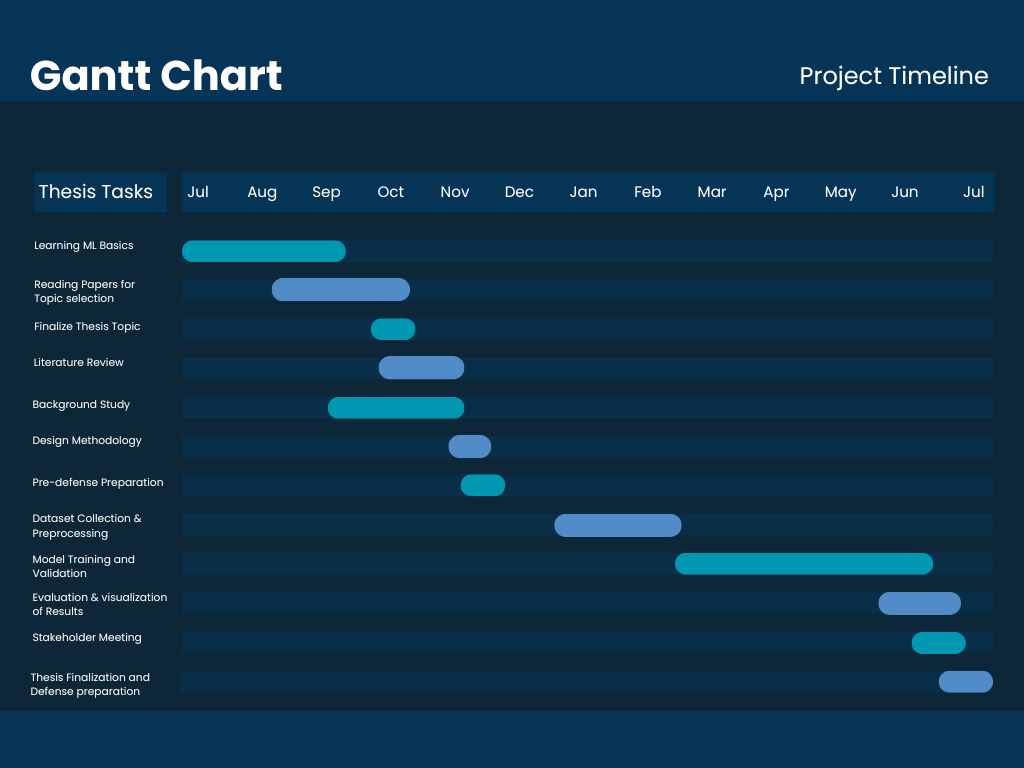
\includegraphics[scale=0.5]{Images/Gantt_Chart.png}
    \caption[Project timeline]{\textbf{Project timeline.} Gantt chart of the project schedule.}
    \label{fig:Gannt Chart}
\end{figure}
\textbf{Deviation Notes (if applicable)}\\
Preprocessing required more time due to the large 3D MRI volumes downloaded from ADNI.
Training time slightly extended because the 3D models require high GPU computation.
Final documentation was completed on schedule.

\section{Budget Estimation}
Although the project used mostly publicly available datasets and open-source tools, a notional budget is included to demonstrate cost awareness. Costs consider hardware resources, computing infrastructure, software services, and miscellaneous expenses.\\
\textbf{Cost Categories}
\begin{itemize}
    \item Hardware / Compute Resources
    \item Software \& ML Tools
    \item Cloud Services / GPU Rental
   \item Miscellaneous (Printing, Transport, Presentation Materials)
\end{itemize}
\textbf{Budget Table(Estimated)}\\
\begin{sloppypar}
\hyphenpenalty=50
\exhyphenpenalty=50
\hyphenchar\font=`\-
\begin{longtable}{|p{4.5cm}|p{2.5cm}|p{3.5cm}|p{3.5cm}|}
\caption{Table of Budget}\\
\hline
\textbf{Item/Resource} & \textbf{Quantity} & \textbf{Unit Cost (BDT)} & \textbf{Total Estimated Cost(BDT)} \\
\hline
High-performance GPU Access(Cloud/Local) & 20 hours & 150 BDT/hour & 3000\\
\hline
External Storage for MRI Files (SSD) & 1 & 4500 & 4500\\
\hline
Software Tools  & -- & Free(Open-source) & 0\\
\hline
Dataset (ADNI) & -- & Free (academic license) & --\\
\hline
Documentation Printing \& Binding & -- & 600 & 600\\
\hline
Transport \& Communication & -- & 1000 & 1000\\
\hline
\textbf{Total Estimated Cost} & -- & -- & \textbf{9100 BDT}\\
\hline
\end{longtable}
\end{sloppypar}

\textbf{Key Notes}\\
The ADNI dataset was accessed freely under an academic license.\\
GPU compute time was the major cost factor due to 3D MRI preprocessing and 3D model training.
All ML frameworks used were fully open-source.\\
\section{Summary}
The project followed a structured timeline beginning with requirement analysis and dataset preparation, progressing through model development using 3D CNN and Vision Transformers, and concluding with evaluation and documentation. The Gantt chart ensured clear planning, logical task distribution, and continuous progress tracking.\\
The project was cost-efficient, with minimal expenses due to the availability of open-source tools and the freely accessible ADNI research dataset. The primary expense involved computing resources for training the deep learning models, particularly the 3D CNN, transformer, and hybrid networks.\\
Overall, the planning and budgeting framework ensured feasible, organized, and efficient execution of the Alzheimer’s Disease Detection Project.





\chapter{Standards and Design Constraints} \label{cha:AccreditationComponents}

This chapter outlines how the project complies with relevant engineering standards, ethical guidelines, and professional practices. It also highlights the design constraints encountered and demonstrates coverage of Complex Engineering Problems (CEP) and Complex Engineering Activities (CEA) through mapping tables aligned with BAETE/ABET accreditation requirements.
\section{Compliance with Standards and Professional Practice}
This project was designed following internationally recognized software, data handling, and ethical standards. The system processes sensitive medical data (MRI scans) and applies deep learning models (3D CNN and Vision Transformer) for Alzheimer’s disease prediction; therefore, compliance with professional engineering practices was essential.\\
The design also incorporates considerations of data privacy, safety, environmental sustainability, fairness in algorithms, and responsible use of computing resources.
\subsection{Software Standards}
The software was developed with reference to the following standards and guidelines. They were used as frameworks for structuring the work; no formal certification was sought.\\
\textbf{ISO/IEC/IEEE 12207 (Software life-cycle processes)}\\
The work followed the life-cycle stages of requirements analysis (Chapter~\ref{cha:SystemAnalysisAndDesignU}), design, implementation, verification, and documentation.\\
\textbf{ISO/IEC 25010 (Software product quality model)}\\
The quality characteristics most relevant to a research pipeline were addressed as follows:
\begin{itemize}
    \item \textbf{Reliability} --- fixed random seeds, saved split files, and fold-wise reporting (mean $\pm$ std).
    \item \textbf{Maintainability} --- modular data, model, training, evaluation, and explainability components behind a common interface.
    \item \textbf{Performance efficiency} --- cached preprocessing, mixed-precision training, and gradient accumulation to fit a 16\,GB GPU.
\end{itemize}
\textbf{Reporting guideline: CLAIM (Checklist for Artificial Intelligence in Medical Imaging)}\\
CLAIM was used as a reference for what to report: data source and curation, subject-level partitioning, reference standard, model and training details, evaluation metrics with variability, and limitations.

\subsection{Data and Imaging Standards}
\textbf{DICOM and NIfTI-1}\\
MRI scanners store images in DICOM; ADNI distributes the pre-processed volumes used here in NIfTI-1 format, which preserves voxel spacing and orientation metadata. The pipeline reads that metadata to reorient every volume to RAS and resample it to isotropic spacing.

\subsection{Other Standards and Regulations}
\textbf{Data privacy and research ethics}\\
ADNI data are de-identified by the ADNI consortium and were accessed under the ADNI Data Use Agreement, with HIPAA de-identification principles as the reference. The hospital scans used in the preliminary external pilot are covered by the ethics statement in Section~\ref{sec:extval}.\\
\textbf{Medical-device and AI regulation (awareness only)}\\
Software that supports diagnosis may fall under medical-device rules --- IEC 62304 (medical-device software life cycle), ISO 14971 (risk management), and the EU AI Act, which treats AI used in medical devices as high-risk. This thesis is a research prototype and makes no compliance claim; the standards are listed to show what clinical deployment would require.\\
\textbf{Ethically aligned design}\\
IEEE 7000 (addressing ethical concerns during system design) informed the practices adopted here: transparent reporting of negative results, explicit statement of limitations, and positioning the system as decision support rather than diagnosis.

\section{Design Constraints}

\subsection{Ethical and Professional Responsibilities}
This project follows established ethical and professional standards to ensure responsible development and fair use of the system. All results are reported honestly, without any form of exaggeration or falsification of accuracy or performance outcomes. The study also respects intellectual property rights by properly citing the ADNI dataset used. To protect privacy, only de-identified MRI scans are used, and no personal or identifiable information appears in this thesis. Class imbalance (MCI is the minority) is addressed with class weighting and macro-F1 reporting; demographic fairness (for example, performance by sex or age group) was not evaluated and is left to future work. Additionally, the system is developed with responsible machine learning practices in mind, and it is clearly stated that the model is intended only for research purposes and should not be used as a clinical diagnostic tool.
\subsection{Environmental and Sustainability Considerations}
The design limits computational and environmental cost in the following ways:
\begin{itemize}
    \item \textbf{Single local GPU.} All training ran on one consumer GPU (RTX 5060 Ti, 16\,GB) rather than a multi-GPU cluster.
    \item \textbf{Early stopping.} Training stops when validation macro-F1 stops improving, avoiding unnecessary epochs.
    \item \textbf{Mixed precision.} Automatic mixed precision reduces memory traffic and computation per step.
    \item \textbf{Cached preprocessing.} The deterministic preprocessing is computed once and reused across epochs, folds, and models.
    \item \textbf{Compact models.} Compact backbones (DenseNet-121, a 6-layer ViT) were preferred over large transformer models.
\end{itemize}

\subsection{Health and Safety Considerations}
Although this is primarily a software-based project, several important health and safety aspects were carefully considered. The ADNI data used for training and evaluation are de-identified and were collected under ADNI's ethical approvals; the ethical basis for the small hospital pilot is stated separately in Section~\ref{sec:extval}. In cases where laboratory resources such as GPU machines were used, standard safety practices were followed, including preventing overheating, maintaining proper ventilation, and ensuring secure electrical connections. User safety was also taken into account, as the system does not make autonomous clinical decisions and functions only as an analytical support tool rather than a medical diagnostic system. Additionally, no raw clinical identifiers are used, and imaging data are kept on the project workstation and not redistributed, in line with the ADNI Data Use Agreement.

\section{Complex Engineering Problem (CEP) Coverage}
This project meets the characteristics of a Complex Engineering Problem (CEP) through its involvement with large-scale, high-dimensional MRI data; advanced AI models; conflicting technical constraints; and multi-disciplinary medical–engineering aspects.\\
Below is the required BAETE CEP mapping.
\begin{sloppypar}
\hyphenpenalty=50
\exhyphenpenalty=50
\hyphenchar\font=`\-
\begin{longtable}{|p{3.2cm}|p{6.6cm}|p{2.1cm}|p{2.1cm}|}
\caption{Complex Engineering Problems (Ps): mapping with Knowledge Profiles (K), CLOs, and PLOs}\\
\hline
\textbf{Ps Attribute} & \textbf{How Ps are Addressed in the Project} & \textbf{CLOs} & \textbf{PLOs}\\
\hline
P1: Depth of Knowledge Required & Requires advanced knowledge of ML, 3D CNN/ViT architectures, mathematical modeling, and 3D MRI preprocessing. [K3, K4, K6, K8] & CLO1, CLO2, CLO7 & PLO1, PLO2, PLO5\\
\hline
P3: Depth of Analysis Required & The problem has no obvious solution and requires custom architecture design and fusion strategies. [K3] & CLO2, CLO7 & PLO2, PLO3, PLO4\\
\hline
P4: Familiarity of Issues & Involves unfamiliar 3D medical imaging tasks such as MRI preprocessing, Alzheimer's classification, subject-level evaluation, and XAI interpretation. [K4, K6, K8] & CLO1, CLO7 & PLO4, PLO5, PLO12\\
\hline
P6: Stakeholder Involvement & Various stakeholders are involved --- practising clinicians gave informal feedback on the model and its explanations, and a collaborating diagnostic centre supplied pilot data. [K5, K8] & CLO2, CLO5, CLO6 & PLO6, PLO8, PLO10\\
\hline
P7: Interdependence & Multiple interdependent modules --- preprocessing, 3D feature extraction, fusion, classification, evaluation, and XAI --- work together as one complete system pipeline. [K5, K6] & CLO3, CLO7 & PLO3, PLO5\\
\hline
\end{longtable}
\end{sloppypar}


\section{Complex Engineering Activities (CEA) Coverage}
The project includes complex engineering activities such as system design, experimentation, computational modeling, and performance evaluation.
\begin{sloppypar}
\hyphenpenalty=50
\exhyphenpenalty=50
\hyphenchar\font=`\-
\begin{longtable}{|p{3.2cm}|p{6.6cm}|p{2.1cm}|p{2.1cm}|}
\caption{Complex Engineering Activities (As): mapping with CLOs and PLOs}\\
\hline
\textbf{As Attribute} & \textbf{How As are Addressed in the Project} & \textbf{CLOs} & \textbf{PLOs}\\
\hline
A1: Range of Resources & Used the ADNI MRI dataset, GPU hardware, PyTorch, and medical-imaging tools such as NiBabel/MONAI. & CLO2, CLO7 & PLO3, PLO5\\
\hline
A2: Level of Interaction & Integrated 3D MRI preprocessing, model training, feature extraction, evaluation, and XAI into one workflow. & CLO2, CLO7 & PLO2, PLO3, PLO5\\
\hline
A4: Consequences for Society and Environment & Supports Alzheimer's decision-support research by assisting clinicians and improving model transparency. & CLO4, CLO5 & PLO6, PLO8\\
\hline
A5: Familiarity & Extends beyond prior experience through 3D MRI processing, Transformer-based modeling, subject-level evaluation, and XAI. & CLO1, CLO7 & PLO1, PLO4, PLO12\\
\hline
\end{longtable}
\end{sloppypar}


\section{Summary}
This chapter demonstrated how the project fulfills the following:\\
\textbf{Knowledge Profiles (K1–K8)}\\
\begin{itemize}
    \item K1: The project applies natural science knowledge through understanding MRI physics, brain anatomy, and       Alzheimer’s pathology.
    \item K2: The work uses mathematics, statistics, and computational science for deep learning, voxel              processing, normalization, and performance evaluation.
    \item K3: Core engineering fundamentals such as convolution theory, transformer attention mechanisms, and               algorithmic modeling are covered.
    \item K4: Specialist engineering knowledge of 3D medical image analysis, transformer architectures, and volumetric preprocessing is applied.
    \item K5: The project involves engineering design of a functional hybrid 3D CNN–ViT architecture and a full MRI processing pipeline.
    \item K6: The project uses engineering practice tools including Python, PyTorch, MONAI, GPU computing, and medical imaging libraries.
    \item K7: The system raises healthcare, ethical, and societal considerations involving medical data privacy,     clinical impact, and responsible AI.
    \item K8: The project requires engaging with current research literature on CNNs, transformers, MRI-based Alzheimer's classification, data leakage in evaluation, and explainable AI.
\end{itemize}
\textbf{Complex Engineering Problems (P1–P7)}\\
The proposed research on Alzheimer’s disease detection using 3D MRI scans qualifies as a Complex Engineering Problem due to several contributing factors. It requires in-depth knowledge of neuroimaging, volumetric preprocessing, and advanced deep learning architectures, justifying the inclusion of P1. The project also involves multiple stakeholders --- clinicians who gave feedback on the model and its explanations, and a diagnostic centre that supplied pilot data --- corresponding to P6. Developing a hybrid 3D CNN–Vision Transformer model demands significant analytical depth and original design decisions, fulfilling P3, while the unfamiliar nature of medical imaging analysis supports P4. Additionally, the project consists of multiple interdependent modules—ranging from data preprocessing to feature extraction, fusion, and explainability—corresponding to P7. Together, these attributes demonstrate that the project involves multifaceted engineering complexity beyond routine problem-solving.\\
\textbf{Complex Engineering Activities (A1–A5)}\\
The study also satisfies several criteria for Complex Engineering Activities. It makes use of diverse computational, informational, and technological resources, including a large-scale 3D MRI dataset, GPU hardware, and specialized imaging and deep learning libraries, which reflect A1. The project requires resolving complex interactions between preprocessing workflows, model components, and dataset variations, thereby involving A2. The potential impact on early Alzheimer detection and healthcare decision-making highlights the broader societal significance described in A4. Finally, the project incorporates advanced engineering tasks that extend beyond typical undergraduate experience, fulfilling A5. These characteristics collectively demonstrate that the work constitutes a complex engineering activity involving creativity, technical depth, and impactful application.

















\chapter{Conclusion and Future Work} \label{cha:ConclusionAndFutureWork}

This chapter presents the concluding remarks of the study and outlines directions for future work. It summarizes the objectives, methodological contributions, and experimental findings of the Alzheimer's detection framework, reflects on what the results actually show, acknowledges the limitations encountered, and proposes enhancements to guide further research.
\section{Summary of the Work}
This research developed and benchmarked a family of fully three-dimensional deep-learning models for Alzheimer's Disease classification from structural MRI. Working on the ADNI dataset (1{,}132 T1-weighted volumes from 395 subjects), five architectures—a 3D DenseNet CNN, a MedicalNet-pretrained 3D ResNet, a 3D Vision Transformer, a Swin Transformer, and the proposed hybrid 3D CNN–ViT—were trained on an identical pipeline and compared under a strict subject-level five-fold protocol. Two tasks were studied: binary CN-vs-AD and three-class CN/MCI/AD. The design deliberately prioritized an \emph{honest}, leakage-free comparison over a headline accuracy number, and integrated 3D Grad-CAM and related attribution methods for interpretability. The study demonstrates that combining local CNN features with global transformer context yields the best binary result, while quantifying exactly how much—and how little—that hybridization helps.

\section{Key Findings and Contributions}
The experiments produced several clear findings. The proposed \textbf{hybrid 3D CNN–ViT achieved the best binary CN-vs-AD performance ($82.2\%$ accuracy, macro-F1 $0.80$)}, but its margin over a strong from-scratch 3D DenseNet ($81.0\%$) was within one standard deviation—so hybridization gives a small, consistent edge rather than a dramatic gain. On the three-class task the honest ceiling was $\sim\!57.7\%$ (Swin), with MCI, the transitional stage, acting as the dominant source of confusion. Two instructive negative results emerged: the MedicalNet-\emph{pretrained} ResNet underperformed the from-scratch CNN and was highly unstable across folds—traced partly to an early-stopping artifact rather than the architecture itself—and a from-scratch 3D ViT collapsed to near-chance on the three-class task, confirming that data-hungry transformers need large-scale pretraining.

The contributions of this study are:
\begin{enumerate}
    \item \textbf{A rigorous, leakage-free benchmark.} A single-source ADNI cohort evaluated with subject-level five-fold cross-validation and an identical pipeline across all models, giving a genuinely fair single-vs-hybrid comparison—in contrast to the slice-level, leakage-prone evaluations that dominate the literature~\cite{wen2020convolutional,yagis2021effect}.
    \item \textbf{The hybrid 3D CNN–ViT design and its honest assessment.} The 3D CNN branch learns localized textures (hippocampal shrinkage, cortical thinning, ventricular enlargement) while the 3D ViT branch models long-range dependencies; late-concatenation fusion of the two is shown to give the best—if modest—binary result.
    \item \textbf{An explainability study.} 3D Grad-CAM, Integrated Gradients, and attention rollout localize model attention to medial-temporal and ventricular regions consistent with AD pathology, with the pipeline's limitations (no skull-stripping, coarse spatial regions) stated explicitly.
    \item \textbf{A reproducible, config-driven codebase} that regenerates the curated labels, subject-level splits, all model runs, and every figure.
\end{enumerate}

\section{Limitations of the Study}
Several limitations should be acknowledged. The cohort, though standard, is small (395 subjects; only 80 MCI), which caps three-class performance and makes transformer training difficult. The single-site ADNI focus keeps the labels and protocol clean; a first attempt at external validation on independent hospital scans (Section~\ref{sec:extval}) was constrained by a severe modality/domain shift and is reported below as a preliminary result rather than a demonstration of transfer. The 16\,GB GPU budget constrained input resolution ($96^3$–$128^3$) and batch size, and limited the number of experiments—so a few model$\times$task cells (e.g., some standalone and hybrid three-class runs) remain to be completed. The pretrained-ResNet result is confounded by an early-stopping artifact, and because the ADNI volumes are not skull-stripped or atlas-registered, the explainability maps report importance over coarse spatial regions rather than named anatomical ROIs. These are documented honestly rather than hidden.

\section{Preliminary External Validation on Independent Hospital Data}\label{sec:extval}
To probe generalization beyond ADNI, the trained models were applied to a small set of real clinical MRI scans obtained from a collaborating diagnostic center, \textbf{Comfort Diagnostic Center}. Weak diagnostic labels for these scans were derived from routine radiology reports under the guidance of a collaborating clinician, \textbf{Dr.\ Ziaur Rahman} (Physician \& Surgeon); the labels are termed \emph{weak} because they come from clinical reports rather than a formal research diagnostic protocol. This exercise is reported transparently as a \emph{preliminary} pilot test, not as a headline result. Table~\ref{tab:extval} summarises the outcome across models.

\begin{table}[H]
\centering
\caption{\textbf{Preliminary hospital external-testing results.} Each ADNI-trained model applied to the hospital pilot set ($n=8$: 4 CN, 4 MCI; no AD cases). ``Hosp AUC$^{*}$'' is CN-vs-MCI ranking quality on the pilot set.}
\label{tab:extval}
\resizebox{\textwidth}{!}{%
\begin{tabular}{|l|c|c|c|c|c|}
\hline
\textbf{Model} & \textbf{Trained for} & \textbf{ADNI 5-fold} & \textbf{Hosp 3-class} & \textbf{Hosp CN-vs-MCI} & \textbf{Hosp AUC$^{*}$} \\
\hline
Swin & 3-class & 57.7\% & 38\% (3/8) & 75\% (6/8) & 0.62 \\
CNN (DenseNet) & 3-class & 57.2\% & 25\% (2/8) & 38\% (3/8) & 0.50 \\
ViT & 3-class & 28.6\% & 25\% (2/8) & 50\% (4/8) & 0.12 \\
CNN (DenseNet) & binary & 81.0\% & n/a & 75\% (6/8) & 0.94 \\
ResNet-18 (MedicalNet) & binary & 69.8\% & n/a & 50\% (4/8) & 0.94 \\
\hline
\end{tabular}%
}
\end{table}
\noindent{\footnotesize $^{*}$The apparently high 0.94 binary AUC is \textbf{age-confounded} and must \emph{not} be read as evidence of transfer (see below).}

The attempt surfaced a severe \textbf{domain shift}. Whereas the models were trained on 3\,T, 3D T1-weighted MPRAGE volumes at $\sim$1\,mm isotropic resolution, the hospital scans were 1.5\,T, 2D T1-FLAIR acquisitions of roughly 20 slices at 5--6\,mm slice thickness (about $12\times$ anisotropic) --- a fundamentally different modality and resolution regime. Only 8 studies were usable (4 CN, 4 MCI; no AD cases were available), and three-class accuracy fell to chance ($\le$3/8 for every model). The seemingly high binary CN-vs-MCI AUC of 0.94 is \emph{not} evidence of transfer: the CN and MCI subgroups are strongly \textbf{age-confounded} (mean age $\sim$35\,years for CN vs.\ $\sim$68\,years for MCI), so the model is largely tracking age-related atrophy rather than disease, and the sample is far too small for a reliable estimate. The one mild positive is that the binary model assigned a low AD probability ($<0.17$) to all four CN subjects --- it did not raise false AD alarms --- though with no AD cases present, sensitivity could not be assessed.

The honest reading is that this preliminary test does \emph{not} demonstrate transfer; rather, it shows how sharply performance degrades when the acquisition protocol differs from the training distribution, while establishing a realistic data-sharing pathway with the hospital. A meaningful external validation requires 3\,T, 3D volumetric T1-weighted scans with confirmed, research-grade labels including AD cases, which is set out as future work below.

\section{Recommendations and Future Work}
Future work follows directly from these limitations. First, add a min-epoch guard before early stopping and re-evaluate the pretrained backbones, and complete the remaining model$\times$task runs so every cell of the comparison is filled. Second, run the skull-stripping and MNI-registration ablations and initialize the Swin encoder from self-supervised pretrained weights, both of which are expected to raise accuracy and sharpen the explainability maps to true anatomical ROIs. Third, extend the external validation begun here: collect 3\,T, 3D T1-weighted scans with research-grade labels (including AD cases) from the collaborating hospital, and additionally validate on public independent datasets (e.g., MIRIAD or OASIS), to measure genuine cross-site generalization free of the modality mismatch and age confound described above. Finally, the hybrid can be extended with a tuned cross-attention fusion and with multimodal inputs (PET, cognitive scores) to improve the difficult CN/MCI/AD boundary, and evaluated in a realistic clinical workflow. Together these steps would turn a rigorous benchmark into a stronger, externally validated diagnostic-support tool.






% \chapter{Background Study}\label{cha:BS}
% \input{chapters/background}

% \chapter{Literature review}\label{chap:lit}
% \input{chapters/literature}


% \chapter{Dataset Description}\label{chap:dataset}
% \input{chapters/dataset}

% \chapter{Proposed System\label{cha:design}}
% \input{chapters/project design}

% \chapter{Cost and Time Estimation\label{cha:cost_time}}
% \input{chapters/time_cost}


% \chapter{Results\label{cha:rest}}
% \input{chapters/results}

% \chapter{Conclusions\label{cha:cons}}
% \input{chapters/conclusion}



\chapter*{Code and Data Availability}
\addcontentsline{toc}{chapter}{Code and Data Availability}
The complete source code for this project --- the data-preparation and subject-level split scripts, the five 3D model implementations (3D CNN, pretrained 3D ResNet, 3D ViT, Swin, and the hybrid 3D CNN--ViT), the training and evaluation pipeline, the explainability module, and the figure-generation scripts --- is publicly available at:
\begin{center}
\url{https://github.com/SamuelCormaken/Deep-Learning-for-Alzheimers-MRI}
\end{center}
Every experiment is driven by a version-controlled YAML configuration file; the exact hyperparameters, subject-level split files, and step-by-step reproduction instructions are documented in the Reproducibility appendix. The ADNI MRI scans themselves cannot be redistributed and must be obtained directly from the ADNI archive (\url{https://adni.loni.usc.edu}) under its Data Use Agreement; the repository therefore contains only source code and the derived label and cross-validation split files, not any patient imaging data.

\bibliographystyle{plain}

\bibliography{references.bib}


\appendix 
% \input{chapters/appendix}
\chapter{Questionnaire}

\begin{center}
\textbf{\Large Questionnaire for Alzheimer’s Disease Detection Using 3D MRI and Hybrid CNN--ViT Model}
\end{center}

\vspace{0.3cm}

\noindent\textbf{Thesis Title:} Alzheimer's Detection Using 3D CNN--ViT With Explainable AI

\noindent\textbf{Purpose:}  
This questionnaire aims to gather expert and user perspectives on the use of 3D MRI, hybrid deep learning models, and explainable AI for Alzheimer’s disease detection.

\vspace{0.5cm}

\section*{Section A: Participant Information}

\begin{enumerate}
\item Profession / Role:\\
$\square$ Medical Doctor \hspace{0.3cm}
$\square$ Neurologist / Radiologist \hspace{0.3cm}
$\square$ AI/ML Researcher \hspace{0.3cm}
$\square$ Student \hspace{0.3cm}
$\square$ Other: \underline{\hspace{3cm}}

\end{enumerate}


\section*{Section B: Understanding of Alzheimer’s \& Imaging}

\begin{enumerate}[resume]
\item How important would 3D MRI be in early Alzheimer’s detection?\\
$\square$ Moderately important \hspace{0.3cm}
$\square$ Very important \hspace{0.3cm}
$\square$ Essential

\item Which brain regions are most informative for AD detection? (Select any)\\
$\square$ Hippocampus \hspace{0.3cm}
$\square$ Temporal Lobe \hspace{0.3cm}
$\square$ Ventricular Regions \hspace{0.3cm}
$\square$ Whole-brain Atrophy

\item Should AD detection rely more on:\\
$\square$ 3D MRI volumes \hspace{0.3cm}
$\square$ 2D MRI slices \hspace{0.3cm}
$\square$ Combination of both
\end{enumerate}


\section*{Section C: AI-Based Diagnosis}

\begin{enumerate}[resume]
\item How confident are you in using AI tools for Alzheimer’s diagnosis?\\
$\square$ Slightly confident \hspace{0.3cm}
$\square$ Moderately confident \hspace{0.3cm}
$\square$ Highly confident

\item Do you think combining CNN and Vision Transformers is beneficial for MRI-based diagnosis?\\
$\square$ No \hspace{0.3cm}
$\square$ Maybe \hspace{0.3cm}
$\square$ Yes

\item What level of explainability do you expect from the AI model (e.g., heatmaps)?\\
$\square$ Minimal \hspace{0.3cm}
$\square$ Moderate \hspace{0.3cm}
$\square$ High / Clinically interpretable
\end{enumerate}


\section*{Section D: Tools and Diagnostic Modalities}

\begin{enumerate}[resume]
\item Which diagnostic tool holds the most long-term promise for Alzheimer’s detection?\\
$\square$ MRI \hspace{0.3cm}
$\square$ PET Scan \hspace{0.3cm}
$\square$ EEG \hspace{0.3cm}
$\square$ Genetics / Biomarkers \hspace{0.3cm}
$\square$ Cognitive Testing

\item Should patients be imaged during:\\
$\square$ Resting-state MRI \hspace{0.3cm}
$\square$ Task-based MRI (e.g., memory tasks)

\underline{\hspace{10cm}}
\end{enumerate}


\section*{Section E: Concerns, Ethics, and Future Directions}

\begin{enumerate}[resume]
\item What is your biggest concern about AI-based Alzheimer’s diagnosis?\\
$\square$ Misdiagnosis / False predictions \hspace{0.3cm}
$\square$ Ethical or legal issues \hspace{0.3cm}
$\square$ Data privacy \hspace{0.3cm}
$\square$ Over-reliance on AI

\item Do you believe an early-detection AI system would benefit patients and clinicians?\\
$\square$ No \hspace{0.3cm}
$\square$ Partially \hspace{0.3cm}
$\square$ Yes
\end{enumerate}

\section*{Section F: Final Feedback}

\begin{enumerate}[resume]
\item Additional comments or suggestions:\\[0.3cm]
\underline{\hspace{10cm}}\\[0.3cm]
\underline{\hspace{10cm}}
\end{enumerate}

\vspace{0.6cm}
\section*{Completed Expert Questionnaire and Attestation}
\noindent The questionnaire above was prepared for future use; its aggregate responses are not analysed in this thesis. Separately, the following open-ended domain interview was completed and signed by \textbf{Dr.\ Ziaur Rahman} (Physician \& Surgeon, Comfort Diagnostic Center), the clinician who guided the labelling of the hospital scans used in the preliminary external-validation study (Section~\ref{sec:extval}). The responses are reproduced verbatim.

\begin{enumerate}
\item \textbf{What is Alzheimer's disease in general?}\\
Alzheimer's disease is a progressive brain disorder that gradually destroys memory and thinking ability. It is the most common cause of dementia in older adults.

\item \textbf{Why is Alzheimer's considered a neurodegenerative disorder?}\\
Alzheimer's is considered a neurodegenerative disorder because brain cells gradually become damaged and die over time, causing continuous loss of brain function.

\item \textbf{What are the early symptoms of Alzheimer's disease?}\\
Early symptoms include short-term memory loss; patients may also have difficulty finding words or solving problems.

\item \textbf{Which brain region is first affected in Alzheimer's disease?}\\
The hippocampus is usually the first brain region affected, and it is responsible for memory formation, thus memory loss occurs.

\item \textbf{What preliminary tests are used to detect Alzheimer's disease?}\\
Doctors begin with medical history, physical examination, cognitive tests such as the MMSE, blood tests, and brain images like MRI.

\item \textbf{Why is MRI used in Alzheimer's diagnosis?}\\
MRI helps to detect brain shrinkage, mostly in the hippocampus, and rules out other conditions like stroke or brain tumors.

\item \textbf{What MRI changes indicate Alzheimer's disease?}\\
MRI shows shrinkage of the hippocampus, widening of the brain ventricles, and overall brain atrophy, mostly in the temporal and parietal regions.

\item \textbf{What are the current diagnostic criteria for Alzheimer's disease?}\\
Diagnosis is based on clinical symptoms, cognitive assessment, medical history, brain imaging, and sometimes biomarkers from PET scans or cerebrospinal fluid.

\item \textbf{Can MRI alone confirm Alzheimer's disease?}\\
MRI provides important structural information, but it should be combined with clinical evaluation and other diagnostic tests to confirm Alzheimer's.

\item \textbf{What is your opinion about automated Alzheimer's detection?}\\
This can be a valuable tool for early detection and assisting doctors. It should support clinical decision-making rather than replacing experts.

\item \textbf{Why is early detection of Alzheimer's disease important?}\\
Early diagnosis allows patients to receive treatments sooner, plan for future care, manage symptoms effectively, and improve their quality of life.
\end{enumerate}

\vspace{0.6cm}
\noindent\textbf{Respondent Attestation.} The responses above reflect my professional opinion.

\vspace{0.5cm}
\noindent\textbf{Name:} Dr.\ Ziaur Rahman \hfill \textbf{Designation:} Physician \& Surgeon

\vspace{0.4cm}
\noindent\textbf{Institution:} Comfort Diagnostic Center \hfill \textbf{Date:} 02 July 2026

\vspace{0.8cm}
\noindent\textbf{Signature:}\\[0.25cm]

\includegraphics[height=2.2cm]{Images/doctor_signature.png}

\vspace{0.6cm}

\chapter{Reproducibility and Experimental Configuration}\label{app:repro}
Every experiment in this thesis is driven by a version-controlled YAML configuration file, and all models share the same data pipeline and split files. This appendix records the exact settings so the results can be reproduced.

\section*{Common Settings (all runs)}
\begin{itemize}
    \item \textbf{Data:} ADNI, indexed from \texttt{labels.csv}; subject-level 5-fold splits in \texttt{splits/cv5\_binary.json} and \texttt{splits/cv5\_3class.json} (stratified, seed = 42, leakage-asserted).
    \item \textbf{Optimizer:} AdamW; cosine-decay schedule with linear warmup; gradient clipping at 1.0.
    \item \textbf{Memory:} automatic mixed precision, batch size 2 with gradient accumulation 4 (effective batch 8), MONAI \texttt{CacheDataset}.
    \item \textbf{Selection:} early stopping on validation subject-level macro-F1; class weighting / weighted sampling for imbalance.
    \item \textbf{Software:} Python 3.10, PyTorch 2.11 (CUDA 12.8), MONAI 1.6, NiBabel 5.4, scikit-learn 1.4, NumPy 1.26.
    \item \textbf{Hardware:} single NVIDIA RTX 5060 Ti (16 GB), 32 GB RAM.
\end{itemize}

\section*{Per-Run Hyperparameters}
\begin{table}[H]
\centering
\caption{Configuration of the main experimental runs.}
\begin{tabular}{|l|l|c|l|c|c|c|c|}
\hline
\textbf{Run} & \textbf{Task} & \textbf{Input} & \textbf{Loss} & \textbf{Ep.} & \textbf{Warmup} & \textbf{Pat.} & \textbf{wd} \\
\hline
binary\_cnn & binary & $96^3$ & CE + LS 0.1 & 100 & 8 & 18 & 0.03 \\
binary\_resnet\_pretrained & binary & $96^3$ & CE + LS 0.1 & 100 & 8 & 18 & 0.03 \\
binary\_hybrid\_cnnvit & binary & $96^3$ & CE + LS 0.1 & 100 & 8 & 18 & 0.03 \\
binary\_hybrid\_swinvit & binary & $96^3$ & CE + LS 0.1 & 100 & 8 & 18 & 0.03 \\
3class\_cnn & 3-class & $128^3$ & Focal ($\gamma{=}2$) & 80 & 5 & 15 & 0.01 \\
3class\_swin & 3-class & $128^3$ & Focal ($\gamma{=}2$) & 80 & 5 & 15 & 0.01 \\
3class\_vit & 3-class & $96^3$ & Focal ($\gamma{=}2$) & 80 & 5 & 15 & 0.01 \\
\hline
\end{tabular}
\end{table}
All runs use learning rate $1\times10^{-4}$. The CNN backbone is a 3D DenseNet-121; the pretrained ResNet loads MedicalNet weights; the ViT is a compact 3D transformer (hidden 384, 6 layers, 6 heads, $16^3$ patches); the Swin backbone is the SwinUNETR-style encoder; the hybrids fuse two backbones by late concatenation.

\section*{Reproduction Steps}
\begin{enumerate}
    \item Regenerate labels and subject-level splits: \texttt{python scripts/build\_dataset.py}.
    \item Run five-fold cross-validation for a model: \texttt{python scripts/run\_cv.py --config configs/<run>.yaml}.
    \item Aggregate and plot: \texttt{python scripts/figures/make\_all.py}.
\end{enumerate}
Each run writes its config, the split used, per-fold metrics (\texttt{result.json}), a cross-validation summary (\texttt{*\_cv\_summary.json}), TensorBoard logs, and checkpoints under \texttt{experiments/}, so every number and figure in Chapter~\ref{cha:results} is traceable to a specific run.



\end{document}
